
\guideline[g:nontext:figure_caption]
    {Figures: Captions should provide a brief, independent summary.}

\goodbadexample[{\cite[Fig.~2]{Wetzlinger2024ARCH1}}]{
    \IfFileExists{build/figure_caption.pdf}{
        \includegraphics{build/figure_caption.pdf}
    }{
        % This file was created by matlab2tikz.
%
%The latest updates can be retrieved from
%  http://www.mathworks.com/matlabcentral/fileexchange/22022-matlab2tikz-matlab2tikz
%where you can also make suggestions and rate matlab2tikz.
%
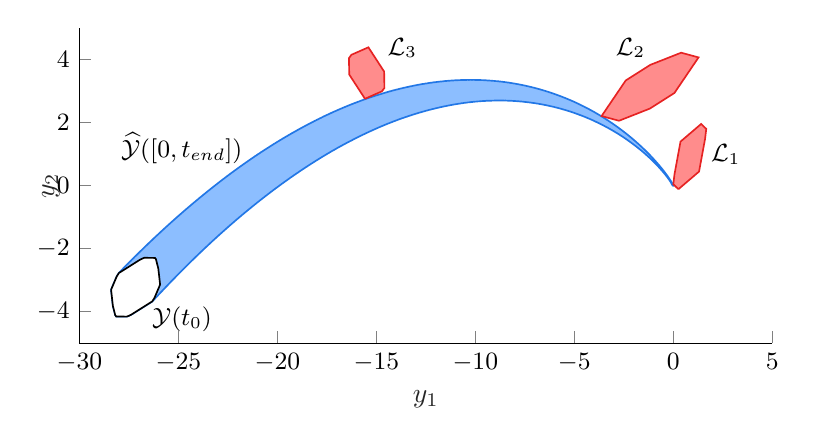
\begin{tikzpicture}[
	every node/.style={font=\small}]

\definecolor{unsafe}{RGB}{255,140,140}			% HSV: 360, 45, 100
\definecolor{unsafeborder}{RGB}{230,34,34}		% HSV: 360, 85, 90
\definecolor{reachouter}{RGB}{140,190,255}		% HSV: 214, 45, 100
\definecolor{reachouterborder}{RGB}{34,119,230}	% HSV: 214, 85, 90

%\draw[red] (-1,-1) grid (13,5.5);
%\draw[red] (10,0) circle(2pt);

% nodes
\node[anchor=west] at (7.9,2.4) {$\mathcal{L}_{1}$};
\node[anchor=south] at (7,3.5) {$\mathcal{L}_{2}$};
\node[anchor=south] at (4.1,3.5) {$\mathcal{L}_{3}$};
\node[anchor=west] at (0.8,0.3) {$\mathcal{Y}(t_0)$};
\node[anchor=south] at (1.3,2.15) {$\widehat{\mathcal{Y}}([0,t_{\text{end}}])$};

\begin{axis}[%
width=8.8cm,
height=4cm,
at={(0,0)},
scale only axis,
xmin=-30.0000,
xmax=5.0000,
xlabel style={font=\color{white!15!black}},
xlabel={$y_1$},
ymin=-5.0000,
ymax=5.0000,
ylabel style={font=\color{white!15!black}, yshift=-15pt},
ylabel={$y_2$},
%axis background/.style={fill=white},
axis x line*=bottom,
axis y line*=left
]

% reachable set
\addplot[semithick,draw=reachouterborder,fill=reachouter, forget plot]
table[row sep=crcr] {%
x	y\\
-27.6085	-4.1574\\
-28.1419	-4.1507\\
-28.1423	-4.1505\\
-28.1904	-4.1084\\
-28.1905	-4.1083\\
-28.3085	-3.8148\\
-28.3088	-3.8137\\
-28.3092	-3.8117\\
-28.3979	-3.3107\\
-28.3979	-3.3105\\
-28.3944	-3.2959\\
-28.3939	-3.2944\\
-28.3937	-3.2937\\
-28.3934	-3.2931\\
-28.3909	-3.2893\\
-28.1132	-2.8791\\
-28.1129	-2.8787\\
-28.0006	-2.7665\\
-27.9994	-2.7653\\
-27.8626	-2.6747\\
-27.8542	-2.6714\\
-27.7225	-2.5848\\
-27.7141	-2.5815\\
-27.5831	-2.4958\\
-27.5748	-2.4926\\
-27.4443	-2.4079\\
-27.436	-2.4048\\
-27.3062	-2.321\\
-27.298	-2.318\\
-27.1688	-2.2352\\
-27.1606	-2.2321\\
-27.032	-2.1503\\
-27.0239	-2.1473\\
-26.8959	-2.0664\\
-26.8878	-2.0635\\
-26.7604	-1.9835\\
-26.7524	-1.9807\\
-26.6256	-1.9016\\
-26.6176	-1.8989\\
-26.4914	-1.8207\\
-26.4835	-1.818\\
-26.3579	-1.7407\\
-26.3501	-1.7381\\
-26.225	-1.6617\\
-26.2172	-1.6591\\
-26.0928	-1.5836\\
-26.085	-1.581\\
-25.9612	-1.5064\\
-25.9535	-1.5039\\
-25.8302	-1.4302\\
-25.8226	-1.4278\\
-25.6999	-1.3549\\
-25.6923	-1.3525\\
-25.5702	-1.2804\\
-25.5626	-1.2781\\
-25.4411	-1.2069\\
-25.4336	-1.2046\\
-25.3126	-1.1343\\
-25.3052	-1.1321\\
-25.1848	-1.0625\\
-25.1774	-1.0604\\
-25.0576	-0.9916\\
-25.0502	-0.9895\\
-24.931	-0.9216\\
-24.9237	-0.9195\\
-24.805	-0.8524\\
-24.7977	-0.8504\\
-24.6796	-0.7841\\
-24.6724	-0.7822\\
-24.5548	-0.7166\\
-24.5476	-0.7147\\
-24.4306	-0.65\\
-24.4235	-0.6481\\
-24.3071	-0.5842\\
-24.3	-0.5823\\
-24.1841	-0.5191\\
-24.1771	-0.5174\\
-24.0617	-0.4549\\
-24.0547	-0.4532\\
-23.9399	-0.3915\\
-23.933	-0.3898\\
-23.8187	-0.3289\\
-23.8118	-0.3272\\
-23.6981	-0.2671\\
-23.6912	-0.2655\\
-23.5781	-0.206\\
-23.5713	-0.2044\\
-23.4586	-0.1457\\
-23.4519	-0.1442\\
-23.3398	-0.0862\\
-23.333	-0.0847\\
-23.2215	-0.0274\\
-23.2148	-0.026\\
-23.1038	0.0306\\
-23.0971	0.032\\
-22.9866	0.0879\\
-22.9821	0.0888\\
-22.841	0.1596\\
-22.8327	0.1613\\
-22.6963	0.2291\\
-22.6881	0.2307\\
-22.5524	0.2974\\
-22.5443	0.2989\\
-22.4094	0.3646\\
-22.4013	0.3661\\
-22.2673	0.4307\\
-22.2593	0.4322\\
-22.126	0.4958\\
-22.1181	0.4972\\
-21.9856	0.5598\\
-21.9777	0.5611\\
-21.8461	0.6227\\
-21.8383	0.624\\
-21.7074	0.6847\\
-21.6996	0.6859\\
-21.5695	0.7455\\
-21.5618	0.7467\\
-21.4325	0.8054\\
-21.4267	0.8063\\
-21.2692	0.877\\
-21.2601	0.8782\\
-21.1071	0.9461\\
-21.098	0.9473\\
-20.9462	1.0138\\
-20.9372	1.0149\\
-20.7864	1.0801\\
-20.7775	1.0812\\
-20.6278	1.1451\\
-20.619	1.1461\\
-20.4704	1.2087\\
-20.4617	1.2096\\
-20.3142	1.271\\
-20.3139	1.271\\
-20.3055	1.2719\\
-20.159	1.332\\
-20.1587	1.3321\\
-20.1504	1.3328\\
-20.0051	1.3918\\
-20.0048	1.3918\\
-19.9965	1.3925\\
-19.8522	1.4502\\
-19.8519	1.4503\\
-19.8437	1.4509\\
-19.7005	1.5075\\
-19.7002	1.5075\\
-19.6921	1.5081\\
-19.5499	1.5635\\
-19.5496	1.5635\\
-19.5415	1.5641\\
-19.4003	1.6183\\
-19.4001	1.6184\\
-19.3921	1.6189\\
-19.2519	1.672\\
-19.2516	1.672\\
-19.2438	1.6724\\
-19.1046	1.7244\\
-19.1043	1.7245\\
-19.0965	1.7249\\
-18.9584	1.7757\\
-18.9581	1.7758\\
-18.9503	1.7761\\
-18.8132	1.8259\\
-18.8129	1.826\\
-18.8052	1.8263\\
-18.6691	1.875\\
-18.6688	1.875\\
-18.6612	1.8753\\
-18.5261	1.923\\
-18.5258	1.923\\
-18.5183	1.9232\\
-18.3841	1.9699\\
-18.3838	1.9699\\
-18.3763	1.9701\\
-18.2432	2.0157\\
-18.2429	2.0157\\
-18.2355	2.0158\\
-18.1033	2.0605\\
-18.103	2.0605\\
-18.0957	2.0606\\
-17.9645	2.1042\\
-17.9642	2.1042\\
-17.9569	2.1043\\
-17.8266	2.1469\\
-17.8264	2.147\\
-17.8214	2.147\\
-17.6445	2.204\\
-17.644	2.204\\
-17.6344	2.2039\\
-17.4641	2.2576\\
-17.4636	2.2577\\
-17.4541	2.2575\\
-17.2855	2.3095\\
-17.285	2.3096\\
-17.2756	2.3094\\
-17.1086	2.3598\\
-17.1082	2.3599\\
-17.0988	2.3596\\
-16.9335	2.4084\\
-16.9331	2.4085\\
-16.9238	2.4081\\
-16.7601	2.4555\\
-16.7597	2.4555\\
-16.7505	2.4551\\
-16.5884	2.5009\\
-16.588	2.501\\
-16.579	2.5005\\
-16.42	2.5444\\
-16.4185	2.5448\\
-16.418	2.5449\\
-16.4091	2.5443\\
-16.2517	2.5868\\
-16.2502	2.5872\\
-16.2497	2.5873\\
-16.2409	2.5867\\
-16.085	2.6278\\
-16.0835	2.6282\\
-16.0831	2.6282\\
-16.0744	2.6275\\
-15.92	2.6673\\
-15.9185	2.6677\\
-15.9181	2.6677\\
-15.9095	2.667\\
-15.7567	2.7054\\
-15.7552	2.7057\\
-15.7548	2.7058\\
-15.7463	2.705\\
-15.5949	2.7421\\
-15.5935	2.7424\\
-15.593	2.7425\\
-15.5847	2.7416\\
-15.4348	2.7774\\
-15.4333	2.7778\\
-15.4329	2.7778\\
-15.4247	2.7769\\
-15.2762	2.8115\\
-15.2748	2.8118\\
-15.2744	2.8118\\
-15.2662	2.8109\\
-15.1192	2.8442\\
-15.1178	2.8445\\
-15.1174	2.8445\\
-15.1093	2.8435\\
-14.9638	2.8757\\
-14.9624	2.8759\\
-14.962	2.876\\
-14.954	2.8749\\
-14.8099	2.9059\\
-14.8085	2.9061\\
-14.8081	2.9062\\
-14.8003	2.9051\\
-14.6576	2.9349\\
-14.6562	2.9351\\
-14.6558	2.9351\\
-14.648	2.934\\
-14.5067	2.9627\\
-14.5054	2.9629\\
-14.5049	2.9629\\
-14.4989	2.962\\
-14.3206	2.997\\
-14.3189	2.9972\\
-14.3184	2.9973\\
-14.3089	2.9958\\
-14.1365	3.0283\\
-14.1348	3.0285\\
-14.1343	3.0286\\
-14.1249	3.027\\
-13.9547	3.0579\\
-13.953	3.0581\\
-13.9524	3.0582\\
-13.9432	3.0566\\
-13.7751	3.0858\\
-13.7734	3.086\\
-13.7729	3.0861\\
-13.7638	3.0844\\
-13.5977	3.1121\\
-13.5956	3.1124\\
-13.5866	3.1106\\
-13.4226	3.1369\\
-13.4221	3.1369\\
-13.4205	3.1371\\
-13.4116	3.1353\\
-13.2497	3.16\\
-13.2491	3.1601\\
-13.2475	3.1602\\
-13.2388	3.1584\\
-13.0789	3.1817\\
-13.0783	3.1818\\
-13.0768	3.1819\\
-13.0696	3.1803\\
-12.877	3.2069\\
-12.8763	3.207\\
-12.8745	3.2071\\
-12.8643	3.2048\\
-12.6779	3.2289\\
-12.6772	3.229\\
-12.6754	3.2291\\
-12.6654	3.2268\\
-12.4818	3.249\\
-12.4811	3.2491\\
-12.4793	3.2492\\
-12.4695	3.2468\\
-12.2886	3.2672\\
-12.2879	3.2673\\
-12.2861	3.2674\\
-12.2765	3.2649\\
-12.0983	3.2836\\
-12.0976	3.2837\\
-12.0958	3.2837\\
-12.0864	3.2812\\
-11.9105	3.2983\\
-11.9084	3.2983\\
-11.8992	3.2958\\
-11.7259	3.3112\\
-11.7238	3.3112\\
-11.7148	3.3087\\
-11.5441	3.3225\\
-11.542	3.3225\\
-11.5332	3.3199\\
-11.3649	3.3322\\
-11.3646	3.3322\\
-11.3629	3.3321\\
-11.3543	3.3295\\
-11.1885	3.3404\\
-11.1869	3.3403\\
-11.1865	3.3403\\
-11.1784	3.3377\\
-11.0651	3.3443\\
-11.0148	3.3471\\
-11.0131	3.347\\
-11.0128	3.347\\
-11.0053	3.3446\\
-10.8933	3.3502\\
-10.8436	3.3524\\
-10.842	3.3522\\
-10.8417	3.3522\\
-10.8348	3.3499\\
-10.724	3.3547\\
-10.6751	3.3563\\
-10.6735	3.3561\\
-10.6732	3.3561\\
-10.6669	3.354\\
-10.5573	3.3578\\
-10.509	3.3589\\
-10.5075	3.3587\\
-10.5072	3.3587\\
-10.5014	3.3567\\
-10.3931	3.3597\\
-10.3455	3.3602\\
-10.344	3.36\\
-10.3437	3.36\\
-10.3385	3.3581\\
-10.2314	3.3603\\
-10.1845	3.3603\\
-10.183	3.3601\\
-10.1827	3.3601\\
-10.1823	3.3599\\
-10.1818	3.3598\\
-10.178	3.3584\\
-10.0722	3.3597\\
-10.0259	3.3592\\
-10.0244	3.359\\
-10.0241	3.359\\
-10.0237	3.3588\\
-10.0233	3.3587\\
-10.0229	3.3585\\
-10.0225	3.3584\\
-10.0221	3.3582\\
-10.0199	3.3574\\
-9.9153	3.358\\
-9.8697	3.357\\
-9.8682	3.3568\\
-9.8679	3.3567\\
-9.8675	3.3566\\
-9.8671	3.3564\\
-9.8667	3.3563\\
-9.8663	3.3561\\
-9.8659	3.356\\
-9.8655	3.3558\\
-9.8651	3.3557\\
-9.8647	3.3555\\
-9.8642	3.3553\\
-9.7608	3.3551\\
-9.7159	3.3537\\
-9.7144	3.3535\\
-9.7141	3.3534\\
-9.7137	3.3533\\
-9.7133	3.3531\\
-9.7129	3.353\\
-9.7125	3.3528\\
-9.7121	3.3527\\
-9.7117	3.3525\\
-9.7113	3.3524\\
-9.7108	3.3522\\
-9.6087	3.3512\\
-9.5644	3.3494\\
-9.5629	3.3492\\
-9.5626	3.3491\\
-9.5622	3.3489\\
-9.5618	3.3488\\
-9.5614	3.3486\\
-9.561	3.3485\\
-9.5606	3.3483\\
-9.5602	3.3482\\
-9.5597	3.348\\
-9.4589	3.3463\\
-9.4152	3.344\\
-9.4137	3.3438\\
-9.4133	3.3436\\
-9.4129	3.3435\\
-9.4125	3.3433\\
-9.4121	3.3432\\
-9.4117	3.343\\
-9.4113	3.3429\\
-9.4109	3.3427\\
-9.3113	3.3404\\
-9.2682	3.3377\\
-9.2668	3.3375\\
-9.2664	3.3373\\
-9.266	3.3372\\
-9.2656	3.337\\
-9.2652	3.3369\\
-9.2648	3.3367\\
-9.2643	3.3366\\
-9.166	3.3336\\
-9.1235	3.3305\\
-9.1221	3.3302\\
-9.1217	3.3301\\
-9.1213	3.3299\\
-9.1209	3.3298\\
-9.1205	3.3296\\
-9.12	3.3295\\
-9.0229	3.3258\\
-8.981	3.3224\\
-8.98	3.3222\\
-8.8358	3.3156\\
-8.7946	3.3117\\
-8.7928	3.3113\\
-8.792	3.3111\\
-8.7916	3.3109\\
-8.7911	3.3108\\
-8.7907	3.3106\\
-8.7903	3.3105\\
-8.7895	3.3101\\
-8.7891	3.31\\
-8.7889	3.3099\\
-8.6525	3.3025\\
-8.6521	3.3025\\
-8.6117	3.2981\\
-8.6099	3.2977\\
-8.6095	3.2976\\
-8.6091	3.2974\\
-8.6087	3.2973\\
-8.6083	3.2971\\
-8.6079	3.297\\
-8.6075	3.2968\\
-8.6071	3.2967\\
-8.6066	3.2965\\
-8.4726	3.2879\\
-8.4722	3.2879\\
-8.4326	3.2831\\
-8.4308	3.2827\\
-8.4304	3.2826\\
-8.43	3.2824\\
-8.4296	3.2823\\
-8.4292	3.2821\\
-8.4288	3.282\\
-8.4284	3.2818\\
-8.4279	3.2816\\
-8.2963	3.2721\\
-8.2959	3.2721\\
-8.257	3.2669\\
-8.2553	3.2664\\
-8.2545	3.2662\\
-8.2541	3.266\\
-8.2537	3.2659\\
-8.2533	3.2657\\
-8.2529	3.2656\\
-8.1235	3.255\\
-8.1232	3.255\\
-8.0851	3.2494\\
-8.0834	3.249\\
-8.0829	3.2488\\
-8.0825	3.2487\\
-8.0821	3.2485\\
-8.0817	3.2484\\
-8.0814	3.2483\\
-7.9543	3.2368\\
-7.954	3.2368\\
-7.9166	3.2308\\
-7.9149	3.2304\\
-7.9145	3.2302\\
-7.9141	3.2301\\
-7.9137	3.2299\\
-7.9135	3.2299\\
-7.7885	3.2175\\
-7.7882	3.2175\\
-7.7515	3.2112\\
-7.7499	3.2107\\
-7.7495	3.2106\\
-7.749	3.2104\\
-7.6261	3.1972\\
-7.6258	3.1971\\
-7.5898	3.1905\\
-7.5882	3.1901\\
-7.5878	3.1899\\
-7.467	3.1759\\
-7.4667	3.1758\\
-7.4314	3.1689\\
-7.43	3.1685\\
-7.3111	3.1537\\
-7.3108	3.1537\\
-7.2762	3.1465\\
-7.2755	3.1463\\
-7.1585	3.1307\\
-7.1581	3.1307\\
-7.1242	3.1232\\
-7.1241	3.1232\\
-7.0089	3.1069\\
-7.0086	3.1069\\
-6.9765	3.0994\\
-6.8624	3.0824\\
-6.8621	3.0823\\
-6.8318	3.075\\
-6.7188	3.0572\\
-6.7185	3.0571\\
-6.69	3.0499\\
-6.579	3.0315\\
-6.5782	3.0314\\
-6.5779	3.0313\\
-6.5512	3.0242\\
-6.4412	3.0051\\
-6.4405	3.005\\
-6.4402	3.0049\\
-6.4151	2.998\\
-6.3063	2.9782\\
-6.3056	2.9781\\
-6.3053	2.978\\
-6.2817	2.9712\\
-6.1742	2.9508\\
-6.1739	2.9508\\
-6.1509	2.9439\\
-6.0447	2.923\\
-6.0444	2.9229\\
-6.0225	2.9161\\
-5.9179	2.8947\\
-5.9177	2.8946\\
-5.8968	2.8879\\
-5.7938	2.8661\\
-5.7935	2.866\\
-5.7735	2.8594\\
-5.6721	2.8371\\
-5.6719	2.837\\
-5.6528	2.8305\\
-5.5554	2.8084\\
-5.553	2.8078\\
-5.5528	2.8078\\
-5.5346	2.8014\\
-5.4387	2.7789\\
-5.4363	2.7783\\
-5.4357	2.7781\\
-5.4218	2.773\\
-5.297	2.7427\\
-5.2941	2.742\\
-5.2937	2.7419\\
-5.2933	2.7417\\
-5.2929	2.7416\\
-5.2925	2.7414\\
-5.2921	2.7413\\
-5.2914	2.741\\
-5.2728	2.734\\
-5.1581	2.7052\\
-5.1553	2.7044\\
-5.1549	2.7043\\
-5.1545	2.7041\\
-5.1541	2.704\\
-5.1537	2.7038\\
-5.1533	2.7037\\
-5.1529	2.7035\\
-5.1525	2.7034\\
-5.1521	2.7032\\
-5.1517	2.7031\\
-5.1513	2.7029\\
-5.1509	2.7028\\
-5.1348	2.6965\\
-5.0228	2.6674\\
-5.0201	2.6666\\
-5.0197	2.6664\\
-5.0193	2.6663\\
-5.0188	2.6661\\
-5.0184	2.666\\
-5.018	2.6658\\
-5.0176	2.6657\\
-5.0172	2.6655\\
-5.0168	2.6654\\
-5.0164	2.6652\\
-5.016	2.6651\\
-5.0157	2.6649\\
-5.0153	2.6648\\
-5.0149	2.6646\\
-5.0145	2.6645\\
-5.0141	2.6643\\
-5.0002	2.6587\\
-4.891	2.6293\\
-4.8883	2.6285\\
-4.8879	2.6284\\
-4.8875	2.6282\\
-4.8871	2.6281\\
-4.8867	2.6279\\
-4.8863	2.6278\\
-4.8859	2.6276\\
-4.8855	2.6275\\
-4.8851	2.6273\\
-4.8847	2.6272\\
-4.8843	2.627\\
-4.8839	2.6269\\
-4.8835	2.6267\\
-4.8831	2.6266\\
-4.8827	2.6264\\
-4.8824	2.6263\\
-4.882	2.6261\\
-4.8816	2.626\\
-4.8808	2.6256\\
-4.8805	2.6255\\
-4.8688	2.6207\\
-4.7626	2.5911\\
-4.76	2.5903\\
-4.7596	2.5902\\
-4.7592	2.59\\
-4.7587	2.5899\\
-4.7583	2.5897\\
-4.7579	2.5896\\
-4.7575	2.5894\\
-4.7571	2.5893\\
-4.7567	2.5891\\
-4.7563	2.589\\
-4.7559	2.5888\\
-4.7555	2.5887\\
-4.7552	2.5885\\
-4.7548	2.5884\\
-4.7544	2.5882\\
-4.754	2.5881\\
-4.7532	2.5877\\
-4.7529	2.5876\\
-4.7525	2.5874\\
-4.7521	2.5873\\
-4.7518	2.5871\\
-4.7514	2.587\\
-4.751	2.5868\\
-4.7507	2.5867\\
-4.7503	2.5865\\
-4.7406	2.5824\\
-4.6375	2.5528\\
-4.6349	2.552\\
-4.6345	2.5518\\
-4.6337	2.5516\\
-4.6333	2.5514\\
-4.6329	2.5513\\
-4.6321	2.5509\\
-4.6317	2.5508\\
-4.6313	2.5506\\
-4.6309	2.5505\\
-4.6305	2.5503\\
-4.6301	2.5502\\
-4.6297	2.55\\
-4.6293	2.5499\\
-4.629	2.5497\\
-4.6286	2.5496\\
-4.6282	2.5494\\
-4.6278	2.5493\\
-4.6275	2.5491\\
-4.6271	2.549\\
-4.6267	2.5488\\
-4.6263	2.5487\\
-4.626	2.5485\\
-4.6256	2.5484\\
-4.6252	2.5482\\
-4.6249	2.5481\\
-4.6245	2.5479\\
-4.6242	2.5478\\
-4.6238	2.5476\\
-4.6235	2.5474\\
-4.6156	2.544\\
-4.5156	2.5145\\
-4.5131	2.5136\\
-4.5127	2.5135\\
-4.5123	2.5133\\
-4.5119	2.5132\\
-4.5115	2.513\\
-4.5111	2.5129\\
-4.5107	2.5127\\
-4.5103	2.5126\\
-4.5099	2.5124\\
-4.5095	2.5123\\
-4.5091	2.5121\\
-4.5087	2.512\\
-4.5083	2.5118\\
-4.5079	2.5117\\
-4.5075	2.5115\\
-4.5072	2.5114\\
-4.5068	2.5112\\
-4.5064	2.5111\\
-4.506	2.5109\\
-4.5056	2.5108\\
-4.5053	2.5106\\
-4.5049	2.5104\\
-4.5045	2.5103\\
-4.5042	2.5101\\
-4.5038	2.51\\
-4.5034	2.5098\\
-4.5031	2.5097\\
-4.5027	2.5095\\
-4.5024	2.5094\\
-4.502	2.5092\\
-4.5017	2.5091\\
-4.5013	2.5089\\
-4.501	2.5088\\
-4.5006	2.5086\\
-4.5003	2.5085\\
-4.4999	2.5083\\
-4.4937	2.5055\\
-4.3969	2.4761\\
-4.3941	2.4751\\
-4.3936	2.4749\\
-4.3932	2.4748\\
-4.3928	2.4746\\
-4.3924	2.4745\\
-4.392	2.4743\\
-4.3916	2.4742\\
-4.3912	2.474\\
-4.3908	2.4739\\
-4.3904	2.4737\\
-4.39	2.4736\\
-4.3896	2.4734\\
-4.3893	2.4733\\
-4.3889	2.4731\\
-4.3885	2.473\\
-4.3881	2.4728\\
-4.3877	2.4727\\
-4.3874	2.4725\\
-4.387	2.4724\\
-4.3862	2.472\\
-4.3859	2.4719\\
-4.3855	2.4717\\
-4.3851	2.4716\\
-4.3848	2.4714\\
-4.3844	2.4713\\
-4.3841	2.4711\\
-4.3837	2.471\\
-4.3833	2.4708\\
-4.383	2.4707\\
-4.3826	2.4705\\
-4.3823	2.4704\\
-4.3819	2.4702\\
-4.3816	2.4701\\
-4.3813	2.4699\\
-4.3809	2.4698\\
-4.3806	2.4696\\
-4.3802	2.4694\\
-4.3799	2.4693\\
-4.3795	2.4691\\
-4.377	2.468\\
-4.2591	2.4311\\
-4.2587	2.4309\\
-4.2583	2.4308\\
-4.2579	2.4306\\
-4.2575	2.4305\\
-4.2571	2.4303\\
-4.2567	2.4302\\
-4.2535	2.429\\
-4.2527	2.4286\\
-4.2523	2.4285\\
-4.2519	2.4283\\
-4.2515	2.4282\\
-4.2511	2.428\\
-4.2507	2.4279\\
-4.2503	2.4277\\
-4.2499	2.4276\\
-4.2496	2.4274\\
-4.2492	2.4273\\
-4.2488	2.4271\\
-4.2484	2.427\\
-4.2481	2.4268\\
-4.2477	2.4267\\
-4.2473	2.4265\\
-4.247	2.4264\\
-4.2466	2.4262\\
-4.2463	2.4261\\
-4.2459	2.4259\\
-4.2455	2.4258\\
-4.2452	2.4256\\
-4.2448	2.4254\\
-4.2445	2.4253\\
-4.2441	2.4251\\
-4.2438	2.425\\
-4.2434	2.4248\\
-4.2431	2.4247\\
-4.2428	2.4245\\
-4.2424	2.4244\\
-4.2421	2.4242\\
-4.2418	2.4241\\
-4.2413	2.4239\\
-4.2397	2.4231\\
-4.2331	2.42\\
-4.125	2.3851\\
-4.1246	2.3849\\
-4.1241	2.3848\\
-4.1237	2.3846\\
-4.1233	2.3845\\
-4.1229	2.3843\\
-4.1225	2.3842\\
-4.1221	2.384\\
-4.1217	2.3839\\
-4.1213	2.3837\\
-4.1209	2.3836\\
-4.1205	2.3834\\
-4.1202	2.3833\\
-4.1198	2.3831\\
-4.117	2.382\\
-4.1166	2.3819\\
-4.1163	2.3817\\
-4.1159	2.3816\\
-4.1155	2.3814\\
-4.1151	2.3813\\
-4.1147	2.3811\\
-4.1144	2.381\\
-4.114	2.3808\\
-4.1136	2.3807\\
-4.1133	2.3805\\
-4.1129	2.3804\\
-4.1125	2.3802\\
-4.1122	2.3801\\
-4.1118	2.3799\\
-4.1115	2.3798\\
-4.1111	2.3796\\
-4.1108	2.3795\\
-4.1104	2.3793\\
-4.1101	2.3791\\
-4.1097	2.379\\
-4.1094	2.3788\\
-4.109	2.3787\\
-4.1087	2.3785\\
-4.1084	2.3784\\
-4.108	2.3782\\
-4.1077	2.3781\\
-4.1069	2.3777\\
-4.1064	2.3775\\
-4.1048	2.3767\\
-4.1044	2.3766\\
-4.0986	2.3737\\
-3.995	2.3392\\
-3.9946	2.3391\\
-3.9942	2.3389\\
-3.9937	2.3388\\
-3.9933	2.3386\\
-3.9929	2.3385\\
-3.9925	2.3383\\
-3.9921	2.3382\\
-3.9917	2.338\\
-3.9913	2.3379\\
-3.9909	2.3377\\
-3.9906	2.3376\\
-3.9902	2.3374\\
-3.9898	2.3373\\
-3.9894	2.3371\\
-3.989	2.337\\
-3.9886	2.3368\\
-3.9882	2.3367\\
-3.9879	2.3365\\
-3.9875	2.3364\\
-3.9845	2.3351\\
-3.9841	2.335\\
-3.9837	2.3348\\
-3.9834	2.3347\\
-3.983	2.3345\\
-3.9826	2.3344\\
-3.9823	2.3342\\
-3.9819	2.3341\\
-3.9816	2.3339\\
-3.9812	2.3338\\
-3.9809	2.3336\\
-3.9805	2.3335\\
-3.9802	2.3333\\
-3.9798	2.3331\\
-3.9795	2.333\\
-3.9791	2.3328\\
-3.9788	2.3327\\
-3.9784	2.3325\\
-3.9781	2.3324\\
-3.9778	2.3322\\
-3.9774	2.332\\
-3.9769	2.3318\\
-3.9765	2.3317\\
-3.9737	2.3303\\
-3.9734	2.3301\\
-3.9724	2.3297\\
-3.972	2.3294\\
-3.9689	2.3279\\
-3.8689	2.2937\\
-3.8685	2.2935\\
-3.8681	2.2934\\
-3.8676	2.2932\\
-3.8672	2.2931\\
-3.8668	2.2929\\
-3.8664	2.2928\\
-3.866	2.2926\\
-3.8656	2.2925\\
-3.8652	2.2923\\
-3.8648	2.2922\\
-3.8645	2.292\\
-3.8641	2.2918\\
-3.8637	2.2917\\
-3.8633	2.2915\\
-3.8629	2.2914\\
-3.8625	2.2912\\
-3.8621	2.2911\\
-3.8618	2.2909\\
-3.8614	2.2908\\
-3.861	2.2906\\
-3.8607	2.2905\\
-3.8603	2.2903\\
-3.8599	2.2902\\
-3.8596	2.29\\
-3.8592	2.2899\\
-3.8563	2.2886\\
-3.8559	2.2885\\
-3.8555	2.2883\\
-3.8552	2.2882\\
-3.8548	2.288\\
-3.8545	2.2879\\
-3.8541	2.2877\\
-3.8538	2.2875\\
-3.8534	2.2874\\
-3.8531	2.2872\\
-3.8528	2.2871\\
-3.8524	2.2869\\
-3.8521	2.2868\\
-3.8518	2.2866\\
-3.8513	2.2864\\
-3.8509	2.2862\\
-3.8505	2.2861\\
-3.8469	2.2843\\
-3.8464	2.2841\\
-3.846	2.2839\\
-3.8455	2.2836\\
-3.8451	2.2834\\
-3.8446	2.2832\\
-3.8442	2.2829\\
-3.8414	2.2815\\
-3.7469	2.2482\\
-3.7464	2.2481\\
-3.746	2.2479\\
-3.7452	2.2477\\
-3.7444	2.2473\\
-3.744	2.2472\\
-3.7436	2.247\\
-3.7432	2.2469\\
-3.7428	2.2467\\
-3.7424	2.2466\\
-3.742	2.2464\\
-3.7416	2.2463\\
-3.7413	2.2461\\
-3.7409	2.246\\
-3.7405	2.2458\\
-3.7401	2.2457\\
-3.7397	2.2455\\
-3.7394	2.2454\\
-3.739	2.2452\\
-3.7386	2.2451\\
-3.7383	2.2449\\
-3.7379	2.2448\\
-3.7375	2.2446\\
-3.7372	2.2445\\
-3.7368	2.2443\\
-3.7364	2.2442\\
-3.7361	2.244\\
-3.7357	2.2439\\
-3.7354	2.2437\\
-3.735	2.2435\\
-3.7347	2.2434\\
-3.7318	2.2421\\
-3.7315	2.242\\
-3.7311	2.2418\\
-3.7308	2.2417\\
-3.7305	2.2415\\
-3.7301	2.2414\\
-3.7298	2.2412\\
-3.7286	2.2406\\
-3.7282	2.2405\\
-3.7277	2.2403\\
-3.7265	2.2397\\
-3.7262	2.2395\\
-3.7254	2.2391\\
-3.7249	2.2389\\
-3.7245	2.2387\\
-3.724	2.2384\\
-3.7236	2.2382\\
-3.7231	2.238\\
-3.7227	2.2378\\
-3.7222	2.2375\\
-3.7214	2.2371\\
-3.7209	2.2369\\
-3.7187	2.2357\\
-3.6282	2.203\\
-3.6278	2.2028\\
-3.6274	2.2027\\
-3.627	2.2025\\
-3.6266	2.2024\\
-3.6262	2.2022\\
-3.6258	2.2021\\
-3.6254	2.2019\\
-3.625	2.2018\\
-3.6246	2.2016\\
-3.6242	2.2015\\
-3.6238	2.2013\\
-3.6234	2.2012\\
-3.623	2.201\\
-3.6226	2.2009\\
-3.6223	2.2007\\
-3.6219	2.2006\\
-3.6215	2.2004\\
-3.6211	2.2003\\
-3.6208	2.2001\\
-3.6204	2.2\\
-3.62	2.1998\\
-3.6197	2.1996\\
-3.6193	2.1995\\
-3.6189	2.1993\\
-3.6186	2.1992\\
-3.6182	2.199\\
-3.6179	2.1989\\
-3.6175	2.1987\\
-3.6171	2.1986\\
-3.6168	2.1984\\
-3.6164	2.1983\\
-3.6161	2.1981\\
-3.6158	2.198\\
-3.6154	2.1978\\
-3.6151	2.1977\\
-3.6147	2.1975\\
-3.6144	2.1974\\
-3.6116	2.1961\\
-3.6092	2.1949\\
-3.6088	2.1948\\
-3.6068	2.1938\\
-3.6063	2.1935\\
-3.6058	2.1933\\
-3.6054	2.1931\\
-3.6049	2.1929\\
-3.6045	2.1926\\
-3.6041	2.1924\\
-3.6036	2.1922\\
-3.6032	2.192\\
-3.6028	2.1917\\
-3.6023	2.1915\\
-3.6015	2.1911\\
-3.6011	2.1908\\
-3.5997	2.1901\\
-3.512	2.1576\\
-3.5116	2.1574\\
-3.5112	2.1573\\
-3.5108	2.1571\\
-3.5104	2.157\\
-3.51	2.1568\\
-3.5096	2.1567\\
-3.5092	2.1565\\
-3.5089	2.1564\\
-3.5085	2.1562\\
-3.5081	2.1561\\
-3.5077	2.1559\\
-3.5073	2.1558\\
-3.507	2.1556\\
-3.5066	2.1555\\
-3.5062	2.1553\\
-3.5058	2.1552\\
-3.5055	2.155\\
-3.5051	2.1549\\
-3.5047	2.1547\\
-3.5044	2.1545\\
-3.504	2.1544\\
-3.5037	2.1542\\
-3.5033	2.1541\\
-3.5029	2.1539\\
-3.5026	2.1538\\
-3.5022	2.1536\\
-3.5019	2.1535\\
-3.5016	2.1533\\
-3.5012	2.1532\\
-3.5009	2.153\\
-3.5005	2.1529\\
-3.5002	2.1527\\
-3.4998	2.1526\\
-3.4995	2.1524\\
-3.4975	2.1514\\
-3.4951	2.1503\\
-3.4947	2.1501\\
-3.4943	2.15\\
-3.4923	2.149\\
-3.4918	2.1487\\
-3.4914	2.1485\\
-3.4909	2.1483\\
-3.4905	2.1481\\
-3.49	2.1478\\
-3.4896	2.1476\\
-3.4891	2.1474\\
-3.4887	2.1472\\
-3.4883	2.1469\\
-3.4879	2.1467\\
-3.4874	2.1465\\
-3.487	2.1463\\
-3.4866	2.146\\
-3.485	2.1452\\
-3.4843	2.1448\\
-3.3998	2.1127\\
-3.3994	2.1126\\
-3.3991	2.1124\\
-3.3987	2.1122\\
-3.3983	2.1121\\
-3.3979	2.1119\\
-3.3975	2.1118\\
-3.3971	2.1116\\
-3.3967	2.1115\\
-3.3964	2.1113\\
-3.396	2.1112\\
-3.3956	2.111\\
-3.3952	2.1109\\
-3.3949	2.1107\\
-3.3945	2.1106\\
-3.3941	2.1104\\
-3.3938	2.1103\\
-3.3934	2.1101\\
-3.393	2.11\\
-3.3927	2.1098\\
-3.3923	2.1097\\
-3.392	2.1095\\
-3.3916	2.1094\\
-3.3913	2.1092\\
-3.3909	2.109\\
-3.3906	2.1089\\
-3.3902	2.1087\\
-3.3899	2.1086\\
-3.3895	2.1084\\
-3.3892	2.1083\\
-3.3889	2.1081\\
-3.3885	2.108\\
-3.3853	2.1064\\
-3.3849	2.1063\\
-3.3845	2.1061\\
-3.3822	2.105\\
-3.3818	2.1048\\
-3.3814	2.1045\\
-3.3809	2.1043\\
-3.3805	2.1041\\
-3.38	2.1039\\
-3.3796	2.1036\\
-3.3791	2.1034\\
-3.3787	2.1032\\
-3.3782	2.103\\
-3.3778	2.1027\\
-3.377	2.1023\\
-3.3765	2.1021\\
-3.3761	2.1018\\
-3.3749	2.1012\\
-3.3745	2.1009\\
-3.3729	2.1001\\
-3.3726	2.0999\\
-3.2908	2.0681\\
-3.2904	2.0679\\
-3.29	2.0678\\
-3.2896	2.0676\\
-3.2892	2.0675\\
-3.2888	2.0673\\
-3.2885	2.0672\\
-3.2881	2.067\\
-3.2877	2.0669\\
-3.2874	2.0667\\
-3.287	2.0665\\
-3.2866	2.0664\\
-3.2863	2.0662\\
-3.2859	2.0661\\
-3.2855	2.0659\\
-3.2852	2.0658\\
-3.2848	2.0656\\
-3.2845	2.0655\\
-3.2841	2.0653\\
-3.2838	2.0652\\
-3.2834	2.065\\
-3.2831	2.0649\\
-3.2827	2.0647\\
-3.2824	2.0646\\
-3.282	2.0644\\
-3.2817	2.0642\\
-3.2814	2.0641\\
-3.281	2.0639\\
-3.2806	2.0638\\
-3.2766	2.0618\\
-3.2761	2.0616\\
-3.2757	2.0614\\
-3.2752	2.0612\\
-3.2726	2.0598\\
-3.2721	2.0596\\
-3.2717	2.0594\\
-3.2712	2.0591\\
-3.2704	2.0587\\
-3.2699	2.0585\\
-3.2695	2.0582\\
-3.2683	2.0576\\
-3.2678	2.0574\\
-3.2674	2.0571\\
-3.2658	2.0563\\
-3.2655	2.056\\
-3.2643	2.0554\\
-3.1855	2.024\\
-3.1851	2.0239\\
-3.1847	2.0237\\
-3.1843	2.0236\\
-3.1839	2.0234\\
-3.1836	2.0232\\
-3.1832	2.0231\\
-3.1828	2.0229\\
-3.1825	2.0228\\
-3.1821	2.0226\\
-3.1817	2.0225\\
-3.1814	2.0223\\
-3.181	2.0222\\
-3.1807	2.022\\
-3.1803	2.0219\\
-3.18	2.0217\\
-3.1796	2.0216\\
-3.1793	2.0214\\
-3.1789	2.0213\\
-3.1786	2.0211\\
-3.1782	2.021\\
-3.1779	2.0208\\
-3.1775	2.0206\\
-3.1772	2.0205\\
-3.1769	2.0203\\
-3.1765	2.0202\\
-3.176	2.02\\
-3.1728	2.0184\\
-3.1725	2.0182\\
-3.1715	2.0178\\
-3.1711	2.0176\\
-3.1706	2.0173\\
-3.1702	2.0171\\
-3.1697	2.0169\\
-3.1693	2.0167\\
-3.1689	2.0164\\
-3.1659	2.0149\\
-3.1654	2.0146\\
-3.1638	2.0138\\
-3.1634	2.0135\\
-3.1618	2.0127\\
-3.1614	2.0124\\
-3.1602	2.0118\\
-3.1597	2.0115\\
-3.1594	2.0113\\
-3.0831	1.9803\\
-3.0827	1.9801\\
-3.0823	1.98\\
-3.0819	1.9798\\
-3.0816	1.9796\\
-3.0812	1.9795\\
-3.0809	1.9793\\
-3.0805	1.9792\\
-3.0801	1.979\\
-3.0798	1.9789\\
-3.0794	1.9787\\
-3.0791	1.9786\\
-3.0787	1.9784\\
-3.0784	1.9783\\
-3.078	1.9781\\
-3.0777	1.978\\
-3.0773	1.9778\\
-3.077	1.9777\\
-3.0767	1.9775\\
-3.0763	1.9774\\
-3.076	1.9772\\
-3.0752	1.9768\\
-3.0747	1.9766\\
-3.0739	1.9762\\
-3.0735	1.9761\\
-3.0723	1.9755\\
-3.072	1.9753\\
-3.0716	1.9751\\
-3.0711	1.9749\\
-3.0706	1.9746\\
-3.0702	1.9744\\
-3.0697	1.9742\\
-3.0693	1.974\\
-3.0688	1.9737\\
-3.068	1.9733\\
-3.0675	1.9731\\
-3.0671	1.9728\\
-3.0663	1.9724\\
-3.0642	1.9713\\
-3.0638	1.9711\\
-3.0634	1.9708\\
-3.0629	1.9706\\
-3.0617	1.97\\
-3.0613	1.9697\\
-3.0605	1.9693\\
-3.0602	1.9691\\
-3.0598	1.9689\\
-3.0594	1.9686\\
-3.0589	1.9684\\
-3.0579	1.9678\\
-3.0578	1.9677\\
-2.9842	1.9371\\
-2.9838	1.937\\
-2.9835	1.9368\\
-2.9831	1.9367\\
-2.9828	1.9365\\
-2.9824	1.9364\\
-2.982	1.9362\\
-2.9817	1.9361\\
-2.9813	1.9359\\
-2.981	1.9358\\
-2.9806	1.9356\\
-2.9803	1.9355\\
-2.98	1.9353\\
-2.9796	1.9352\\
-2.9793	1.935\\
-2.9789	1.9348\\
-2.9786	1.9347\\
-2.9783	1.9345\\
-2.9778	1.9343\\
-2.9774	1.9342\\
-2.9734	1.9322\\
-2.9729	1.932\\
-2.9725	1.9318\\
-2.972	1.9315\\
-2.9716	1.9313\\
-2.9711	1.9311\\
-2.9707	1.9309\\
-2.9702	1.9306\\
-2.969	1.93\\
-2.9685	1.9297\\
-2.9673	1.9291\\
-2.9669	1.9288\\
-2.9645	1.9275\\
-2.9633	1.9269\\
-2.9629	1.9266\\
-2.9617	1.926\\
-2.9597	1.9248\\
-2.9593	1.9246\\
-2.8881	1.8944\\
-2.8877	1.8942\\
-2.8874	1.8941\\
-2.887	1.8939\\
-2.8867	1.8938\\
-2.8863	1.8936\\
-2.886	1.8935\\
-2.8856	1.8933\\
-2.8853	1.8932\\
-2.8849	1.893\\
-2.8846	1.8928\\
-2.8843	1.8927\\
-2.8839	1.8925\\
-2.8836	1.8924\\
-2.8824	1.8918\\
-2.8819	1.8916\\
-2.8811	1.8912\\
-2.8807	1.8911\\
-2.8803	1.8909\\
-2.88	1.8907\\
-2.8792	1.8903\\
-2.8787	1.8901\\
-2.8783	1.8898\\
-2.8773	1.8894\\
-2.8769	1.8892\\
-2.8765	1.8889\\
-2.876	1.8887\\
-2.8756	1.8885\\
-2.8751	1.8883\\
-2.8747	1.888\\
-2.8735	1.8874\\
-2.873	1.8871\\
-2.8714	1.8863\\
-2.871	1.886\\
-2.8706	1.8858\\
-2.8683	1.8845\\
-2.8675	1.8841\\
-2.8671	1.8838\\
-2.8666	1.8836\\
-2.8651	1.8827\\
-2.8647	1.8824\\
-2.8642	1.8821\\
-2.864	1.882\\
-2.7953	1.8523\\
-2.795	1.8521\\
-2.7946	1.852\\
-2.7943	1.8518\\
-2.7939	1.8517\\
-2.7936	1.8515\\
-2.7932	1.8514\\
-2.7929	1.8512\\
-2.7926	1.8511\\
-2.7922	1.8509\\
-2.7919	1.8508\\
-2.7903	1.85\\
-2.7898	1.8498\\
-2.7886	1.8492\\
-2.7883	1.849\\
-2.7879	1.8489\\
-2.7875	1.8487\\
-2.787	1.8484\\
-2.7866	1.8482\\
-2.7861	1.848\\
-2.7857	1.8478\\
-2.7852	1.8475\\
-2.7848	1.8473\\
-2.7843	1.8471\\
-2.7839	1.8469\\
-2.7835	1.8466\\
-2.783	1.8464\\
-2.7822	1.846\\
-2.7818	1.8457\\
-2.7813	1.8455\\
-2.7801	1.8449\\
-2.7797	1.8446\\
-2.7785	1.844\\
-2.7782	1.8438\\
-2.7778	1.8435\\
-2.7774	1.8433\\
-2.7769	1.843\\
-2.775	1.8419\\
-2.7745	1.8417\\
-2.7725	1.8405\\
-2.7721	1.8402\\
-2.7716	1.8399\\
-2.7055	1.8108\\
-2.7051	1.8106\\
-2.7048	1.8105\\
-2.7044	1.8103\\
-2.7041	1.8101\\
-2.7038	1.81\\
-2.7034	1.8098\\
-2.7031	1.8097\\
-2.7023	1.8093\\
-2.7018	1.8091\\
-2.7006	1.8085\\
-2.7002	1.8084\\
-2.6994	1.808\\
-2.6991	1.8078\\
-2.6987	1.8076\\
-2.6982	1.8074\\
-2.6977	1.8071\\
-2.6973	1.8069\\
-2.6968	1.8067\\
-2.6964	1.8065\\
-2.6959	1.8062\\
-2.6951	1.8058\\
-2.6946	1.8056\\
-2.6942	1.8053\\
-2.6934	1.8049\\
-2.6929	1.8047\\
-2.6925	1.8044\\
-2.6909	1.8036\\
-2.6905	1.8033\\
-2.6893	1.8027\\
-2.689	1.8025\\
-2.6886	1.8022\\
-2.6881	1.802\\
-2.6866	1.8011\\
-2.6848	1.8\\
-2.6838	1.7994\\
-2.6833	1.7992\\
-2.6829	1.7989\\
-2.6824	1.7986\\
-2.6821	1.7984\\
-2.6181	1.7696\\
-2.6177	1.7695\\
-2.6174	1.7693\\
-2.6171	1.7692\\
-2.6167	1.769\\
-2.6162	1.7688\\
-2.6142	1.7678\\
-2.6138	1.7677\\
-2.6122	1.7669\\
-2.6117	1.7666\\
-2.6113	1.7664\\
-2.6108	1.7662\\
-2.6104	1.7659\\
-2.6099	1.7657\\
-2.6091	1.7653\\
-2.6086	1.765\\
-2.6078	1.7646\\
-2.6073	1.7644\\
-2.6069	1.7641\\
-2.6053	1.7633\\
-2.6049	1.763\\
-2.6033	1.7622\\
-2.6029	1.7619\\
-2.6026	1.7617\\
-2.6021	1.7614\\
-2.6016	1.7612\\
-2.5996	1.76\\
-2.5992	1.7597\\
-2.5069	1.7174\\
-2.5041	1.716\\
-2.5037	1.7159\\
-2.5025	1.7153\\
-2.502	1.715\\
-2.5015	1.7148\\
-2.5011	1.7146\\
-2.5006	1.7143\\
-2.4998	1.7139\\
-2.4993	1.7137\\
-2.4989	1.7134\\
-2.4985	1.7132\\
-2.498	1.713\\
-2.4976	1.7128\\
-2.4972	1.7125\\
-2.4956	1.7117\\
-2.4952	1.7114\\
-2.4936	1.7106\\
-2.4932	1.7103\\
-2.4928	1.7101\\
-2.4918	1.7095\\
-2.4913	1.7093\\
-2.4908	1.709\\
-2.4904	1.7087\\
-2.4889	1.7078\\
-2.4885	1.7076\\
-2.488	1.7073\\
-2.4876	1.707\\
-2.4853	1.7056\\
-2.4848	1.7053\\
-2.4844	1.705\\
-2.484	1.7048\\
-2.4835	1.7045\\
-2.4831	1.7042\\
-2.4827	1.704\\
-2.4819	1.7034\\
-2.4815	1.7032\\
-2.4811	1.7029\\
-2.3998	1.6647\\
-2.3982	1.6639\\
-2.3978	1.6638\\
-2.397	1.6634\\
-2.3965	1.6631\\
-2.3961	1.6629\\
-2.3956	1.6627\\
-2.3952	1.6625\\
-2.3947	1.6622\\
-2.3939	1.6618\\
-2.3934	1.6616\\
-2.393	1.6613\\
-2.3926	1.6611\\
-2.3921	1.6609\\
-2.3917	1.6607\\
-2.3913	1.6604\\
-2.3897	1.6596\\
-2.3893	1.6593\\
-2.3877	1.6585\\
-2.3873	1.6582\\
-2.3869	1.658\\
-2.3859	1.6574\\
-2.3854	1.6572\\
-2.3849	1.6569\\
-2.3845	1.6566\\
-2.383	1.6557\\
-2.3826	1.6555\\
-2.3821	1.6552\\
-2.3817	1.6549\\
-2.3812	1.6546\\
-2.3808	1.6544\\
-2.3804	1.6541\\
-2.3799	1.6538\\
-2.3773	1.6521\\
-2.3769	1.6519\\
-2.3765	1.6516\\
-2.376	1.6513\\
-2.3756	1.6511\\
-2.3751	1.6507\\
-2.3746	1.6504\\
-2.3745	1.6503\\
-2.2967	1.6129\\
-2.2951	1.6121\\
-2.2946	1.6119\\
-2.2942	1.6117\\
-2.2937	1.6114\\
-2.2933	1.6112\\
-2.2928	1.611\\
-2.2924	1.6108\\
-2.2919	1.6105\\
-2.2907	1.6099\\
-2.2902	1.6096\\
-2.2886	1.6088\\
-2.2882	1.6085\\
-2.2866	1.6077\\
-2.2862	1.6074\\
-2.2854	1.607\\
-2.2844	1.6064\\
-2.284	1.6061\\
-2.2835	1.6058\\
-2.283	1.6056\\
-2.282	1.605\\
-2.2816	1.6047\\
-2.2811	1.6044\\
-2.2807	1.6042\\
-2.2802	1.6039\\
-2.2798	1.6036\\
-2.2793	1.6033\\
-2.2789	1.6031\\
-2.2785	1.6028\\
-2.278	1.6025\\
-2.2776	1.6022\\
-2.2772	1.602\\
-2.2764	1.6014\\
-2.2743	1.6001\\
-2.2738	1.5997\\
-2.2723	1.5988\\
-2.1983	1.5624\\
-2.1979	1.5622\\
-2.1974	1.562\\
-2.1969	1.5617\\
-2.1965	1.5615\\
-2.196	1.5613\\
-2.1956	1.5611\\
-2.1952	1.5608\\
-2.1947	1.5606\\
-2.1939	1.5602\\
-2.1934	1.5599\\
-2.1922	1.5593\\
-2.1918	1.559\\
-2.1902	1.5582\\
-2.1898	1.5579\\
-2.1882	1.5571\\
-2.1862	1.5559\\
-2.1858	1.5556\\
-2.1853	1.5554\\
-2.1848	1.5551\\
-2.1844	1.5548\\
-2.1834	1.5542\\
-2.183	1.554\\
-2.1825	1.5537\\
-2.1817	1.5531\\
-2.1812	1.5529\\
-2.1804	1.5523\\
-2.18	1.5521\\
-2.1792	1.5515\\
-2.1782	1.5509\\
-2.1777	1.5505\\
-2.1752	1.5489\\
-2.1747	1.5485\\
-2.1744	1.5484\\
-2.1038	1.5129\\
-2.1034	1.5127\\
-2.1029	1.5125\\
-2.1025	1.5122\\
-2.102	1.512\\
-2.1012	1.5116\\
-2.1007	1.5113\\
-2.0995	1.5107\\
-2.099	1.5105\\
-2.0986	1.5102\\
-2.097	1.5094\\
-2.0966	1.5091\\
-2.0962	1.5089\\
-2.0959	1.5087\\
-2.0951	1.5083\\
-2.0926	1.5068\\
-2.0922	1.5065\\
-2.0917	1.5063\\
-2.0912	1.506\\
-2.0908	1.5057\\
-2.0903	1.5054\\
-2.0899	1.5051\\
-2.0894	1.5049\\
-2.089	1.5046\\
-2.0885	1.5043\\
-2.0881	1.504\\
-2.0877	1.5038\\
-2.0873	1.5035\\
-2.0868	1.5032\\
-2.0864	1.503\\
-2.086	1.5027\\
-2.085	1.5021\\
-2.0845	1.5017\\
-2.0841	1.5014\\
-2.0831	1.5008\\
-2.0826	1.5004\\
-2.0806	1.4991\\
-2.0132	1.4646\\
-2.0128	1.4643\\
-2.0124	1.4641\\
-2.0119	1.4639\\
-2.0115	1.4637\\
-2.0111	1.4634\\
-2.0107	1.4632\\
-2.0102	1.463\\
-2.0098	1.4628\\
-2.0094	1.4625\\
-2.0078	1.4617\\
-2.0074	1.4614\\
-2.0062	1.4608\\
-2.0059	1.4606\\
-2.0034	1.4591\\
-2.0029	1.4589\\
-2.0025	1.4586\\
-2.0015	1.458\\
-2.0011	1.4577\\
-2.0006	1.4575\\
-2.0002	1.4572\\
-1.9997	1.4569\\
-1.9993	1.4566\\
-1.9989	1.4564\\
-1.9985	1.4561\\
-1.998	1.4558\\
-1.9976	1.4556\\
-1.9968	1.455\\
-1.9958	1.4544\\
-1.9953	1.454\\
-1.9948	1.4537\\
-1.9944	1.4534\\
-1.9934	1.4528\\
-1.993	1.4524\\
-1.9924	1.4521\\
-1.9919	1.4517\\
-1.9907	1.4509\\
-1.9265	1.4173\\
-1.926	1.4171\\
-1.9252	1.4167\\
-1.9248	1.4164\\
-1.9244	1.4162\\
-1.9239	1.416\\
-1.9235	1.4158\\
-1.9231	1.4155\\
-1.9219	1.4149\\
-1.9216	1.4147\\
-1.9212	1.4144\\
-1.9204	1.414\\
-1.9194	1.4134\\
-1.9189	1.4132\\
-1.9179	1.4126\\
-1.9175	1.4123\\
-1.9165	1.4117\\
-1.9161	1.4115\\
-1.9156	1.4112\\
-1.9152	1.4109\\
-1.9147	1.4106\\
-1.9143	1.4104\\
-1.9138	1.4101\\
-1.913	1.4095\\
-1.9126	1.4093\\
-1.9121	1.409\\
-1.9117	1.4087\\
-1.9113	1.4085\\
-1.9108	1.4081\\
-1.9098	1.4075\\
-1.9094	1.4072\\
-1.9089	1.4068\\
-1.9084	1.4065\\
-1.908	1.4062\\
-1.9075	1.4059\\
-1.907	1.4055\\
-1.9064	1.4051\\
-1.9059	1.4048\\
-1.9054	1.4044\\
-1.9049	1.4041\\
-1.9046	1.4038\\
-1.8433	1.3712\\
-1.8421	1.3706\\
-1.8417	1.3703\\
-1.8401	1.3695\\
-1.8397	1.3692\\
-1.8385	1.3686\\
-1.837	1.3677\\
-1.8366	1.3674\\
-1.8361	1.3672\\
-1.8351	1.3666\\
-1.8347	1.3663\\
-1.8342	1.366\\
-1.8337	1.3658\\
-1.8333	1.3655\\
-1.8328	1.3652\\
-1.8324	1.3649\\
-1.832	1.3647\\
-1.8315	1.3644\\
-1.8307	1.3638\\
-1.8303	1.3636\\
-1.8295	1.363\\
-1.828	1.3621\\
-1.8275	1.3617\\
-1.827	1.3614\\
-1.8266	1.3611\\
-1.8256	1.3605\\
-1.8246	1.3597\\
-1.824	1.3594\\
-1.823	1.3586\\
-1.8225	1.3583\\
-1.822	1.3579\\
-1.7637	1.3263\\
-1.7633	1.3261\\
-1.7629	1.3258\\
-1.7613	1.325\\
-1.7609	1.3247\\
-1.7601	1.3243\\
-1.7586	1.3234\\
-1.7581	1.3232\\
-1.7577	1.3229\\
-1.7562	1.322\\
-1.7558	1.3217\\
-1.7553	1.3215\\
-1.7549	1.3212\\
-1.7544	1.3209\\
-1.754	1.3206\\
-1.7536	1.3204\\
-1.7531	1.3201\\
-1.7527	1.3198\\
-1.7523	1.3196\\
-1.7515	1.319\\
-1.7511	1.3188\\
-1.7505	1.3184\\
-1.7501	1.3181\\
-1.7491	1.3175\\
-1.7486	1.3171\\
-1.7481	1.3168\\
-1.7477	1.3165\\
-1.7472	1.3162\\
-1.7462	1.3154\\
-1.7456	1.3151\\
-1.7446	1.3143\\
-1.7441	1.314\\
-1.7436	1.3136\\
-1.7432	1.3133\\
-1.7429	1.3131\\
-1.6874	1.2825\\
-1.687	1.2822\\
-1.685	1.2812\\
-1.683	1.28\\
-1.6826	1.2797\\
-1.6821	1.2794\\
-1.6816	1.2792\\
-1.6811	1.2789\\
-1.6807	1.2786\\
-1.6802	1.2783\\
-1.6798	1.278\\
-1.6793	1.2778\\
-1.6785	1.2772\\
-1.678	1.2769\\
-1.6776	1.2767\\
-1.6768	1.2761\\
-1.6764	1.2759\\
-1.676	1.2756\\
-1.6755	1.2753\\
-1.675	1.2749\\
-1.673	1.2737\\
-1.6726	1.2733\\
-1.6716	1.2727\\
-1.6711	1.2723\\
-1.6705	1.2719\\
-1.67	1.2715\\
-1.6695	1.2712\\
-1.669	1.2708\\
-1.6685	1.2705\\
-1.6681	1.2701\\
-1.6676	1.2698\\
-1.6672	1.2695\\
-1.6143	1.2398\\
-1.6139	1.2396\\
-1.6135	1.2393\\
-1.6131	1.2391\\
-1.6121	1.2385\\
-1.6116	1.2383\\
-1.6106	1.2377\\
-1.6102	1.2374\\
-1.6092	1.2368\\
-1.6088	1.2366\\
-1.6083	1.2363\\
-1.6079	1.236\\
-1.6074	1.2357\\
-1.607	1.2355\\
-1.6065	1.2352\\
-1.6057	1.2346\\
-1.6053	1.2344\\
-1.6048	1.2341\\
-1.6044	1.2338\\
-1.604	1.2336\\
-1.6035	1.2332\\
-1.6025	1.2326\\
-1.6021	1.2323\\
-1.6016	1.2319\\
-1.6011	1.2316\\
-1.6007	1.2313\\
-1.6002	1.231\\
-1.5997	1.2306\\
-1.5991	1.2303\\
-1.5981	1.2295\\
-1.5976	1.2292\\
-1.5966	1.2284\\
-1.5961	1.2281\\
-1.5957	1.2277\\
-1.5947	1.2271\\
-1.5946	1.227\\
-1.5442	1.1982\\
-1.5432	1.1976\\
-1.5427	1.1974\\
-1.5422	1.1971\\
-1.5418	1.1968\\
-1.5408	1.1962\\
-1.5404	1.1959\\
-1.5399	1.1957\\
-1.5394	1.1954\\
-1.539	1.1951\\
-1.5385	1.1948\\
-1.5381	1.1946\\
-1.5377	1.1943\\
-1.5372	1.194\\
-1.5368	1.1937\\
-1.5364	1.1935\\
-1.5356	1.1929\\
-1.5352	1.1927\\
-1.5347	1.1923\\
-1.5332	1.1914\\
-1.5327	1.191\\
-1.5322	1.1907\\
-1.5318	1.1904\\
-1.5313	1.1901\\
-1.5303	1.1893\\
-1.5297	1.189\\
-1.5292	1.1886\\
-1.5287	1.1883\\
-1.5282	1.1879\\
-1.528	1.1878\\
-1.4616	1.1492\\
-1.4612	1.1489\\
-1.4597	1.148\\
-1.4592	1.1478\\
-1.4588	1.1475\\
-1.4583	1.1472\\
-1.4579	1.1469\\
-1.4574	1.1466\\
-1.457	1.1464\\
-1.4565	1.1461\\
-1.4557	1.1455\\
-1.4552	1.1453\\
-1.4544	1.1447\\
-1.454	1.1445\\
-1.4536	1.1442\\
-1.4526	1.1436\\
-1.4521	1.1432\\
-1.4511	1.1426\\
-1.4507	1.1423\\
-1.4502	1.1419\\
-1.4492	1.1413\\
-1.4482	1.1405\\
-1.4476	1.1402\\
-1.4466	1.1394\\
-1.4462	1.1391\\
-1.4457	1.1387\\
-1.4452	1.1384\\
-1.4448	1.138\\
-1.4438	1.1374\\
-1.4434	1.137\\
-1.4426	1.1364\\
-1.4421	1.136\\
-1.4409	1.1351\\
-1.4407	1.1349\\
-1.3825	1.1004\\
-1.382	1.1001\\
-1.3816	1.0999\\
-1.3806	1.0993\\
-1.3802	1.099\\
-1.3797	1.0987\\
-1.3793	1.0985\\
-1.3788	1.0982\\
-1.378	1.0976\\
-1.3775	1.0974\\
-1.3767	1.0968\\
-1.3763	1.0966\\
-1.3759	1.0963\\
-1.3754	1.096\\
-1.3749	1.0956\\
-1.3734	1.0947\\
-1.373	1.0944\\
-1.3725	1.094\\
-1.3721	1.0937\\
-1.3715	1.0934\\
-1.3705	1.0926\\
-1.37	1.0923\\
-1.369	1.0915\\
-1.3685	1.0912\\
-1.368	1.0908\\
-1.3675	1.0905\\
-1.3671	1.0901\\
-1.3666	1.0898\\
-1.3662	1.0895\\
-1.3657	1.0891\\
-1.3649	1.0885\\
-1.3644	1.0881\\
-1.3628	1.0869\\
-1.3625	1.0866\\
-1.3623	1.0865\\
-1.3075	1.0534\\
-1.307	1.0531\\
-1.3066	1.0528\\
-1.3061	1.0525\\
-1.3057	1.0522\\
-1.3053	1.052\\
-1.3048	1.0517\\
-1.3044	1.0514\\
-1.304	1.0512\\
-1.3035	1.0509\\
-1.3031	1.0506\\
-1.3027	1.0504\\
-1.3023	1.0501\\
-1.3018	1.0498\\
-1.3013	1.0494\\
-1.3003	1.0488\\
-1.2999	1.0485\\
-1.2994	1.0481\\
-1.2989	1.0478\\
-1.2985	1.0475\\
-1.2979	1.0471\\
-1.2974	1.0468\\
-1.2964	1.046\\
-1.2959	1.0457\\
-1.2954	1.0453\\
-1.2949	1.045\\
-1.2944	1.0446\\
-1.2939	1.0443\\
-1.2935	1.0439\\
-1.293	1.0436\\
-1.2926	1.0432\\
-1.2921	1.0429\\
-1.2917	1.0426\\
-1.2913	1.0422\\
-1.2889	1.0404\\
-1.2885	1.04\\
-1.2881	1.0397\\
-1.2365	1.008\\
-1.236	1.0077\\
-1.2356	1.0074\\
-1.2351	1.0071\\
-1.2347	1.0069\\
-1.2339	1.0063\\
-1.2334	1.0061\\
-1.2326	1.0055\\
-1.2311	1.0046\\
-1.2307	1.0042\\
-1.2297	1.0036\\
-1.2293	1.0033\\
-1.2288	1.003\\
-1.2283	1.0026\\
-1.2277	1.0022\\
-1.2272	1.0018\\
-1.2267	1.0015\\
-1.2262	1.0011\\
-1.2257	1.0008\\
-1.2252	1.0004\\
-1.2247	1.0001\\
-1.2243	0.9997\\
-1.2238	0.9994\\
-1.2233	0.999\\
-1.2225	0.9984\\
-1.222	0.998\\
-1.2212	0.9974\\
-1.2208	0.997\\
-1.2207	0.997\\
-1.1571	0.9571\\
-1.1567	0.9569\\
-1.1563	0.9566\\
-1.1558	0.9563\\
-1.1554	0.956\\
-1.155	0.9558\\
-1.1542	0.9552\\
-1.1527	0.9543\\
-1.1522	0.9539\\
-1.1517	0.9536\\
-1.1513	0.9533\\
-1.1508	0.953\\
-1.1504	0.9527\\
-1.1498	0.9523\\
-1.1493	0.9519\\
-1.1488	0.9516\\
-1.1478	0.9508\\
-1.1473	0.9505\\
-1.1468	0.9501\\
-1.1463	0.9498\\
-1.1458	0.9494\\
-1.1454	0.9491\\
-1.1449	0.9487\\
-1.1445	0.9484\\
-1.144	0.9481\\
-1.1436	0.9477\\
-1.1432	0.9474\\
-1.1427	0.9471\\
-1.1423	0.9468\\
-1.1419	0.9464\\
-1.1411	0.9458\\
-1.1408	0.9455\\
-1.1396	0.9446\\
-1.1392	0.9442\\
-1.1368	0.9423\\
-1.0818	0.9071\\
-1.0814	0.9068\\
-1.0808	0.9064\\
-1.0804	0.9062\\
-1.0799	0.9058\\
-1.0789	0.9052\\
-1.0785	0.9049\\
-1.078	0.9045\\
-1.077	0.9039\\
-1.0766	0.9036\\
-1.0761	0.9032\\
-1.0755	0.9028\\
-1.075	0.9025\\
-1.0745	0.9021\\
-1.074	0.9018\\
-1.073	0.901\\
-1.0725	0.9007\\
-1.0721	0.9003\\
-1.0711	0.8997\\
-1.0707	0.8993\\
-1.0703	0.899\\
-1.0698	0.8987\\
-1.0694	0.8983\\
-1.0678	0.8971\\
-1.0674	0.8967\\
-1.0666	0.8961\\
-1.0635	0.8936\\
-1.0631	0.8933\\
-1.0628	0.893\\
-1.0623	0.8926\\
-1.062	0.8924\\
-1.0115	0.8594\\
-1.01	0.8585\\
-1.0094	0.858\\
-1.0084	0.8574\\
-1.008	0.8571\\
-1.0075	0.8567\\
-1.007	0.8564\\
-1.0064	0.856\\
-1.0059	0.8556\\
-1.0054	0.8553\\
-1.0044	0.8545\\
-1.0039	0.8542\\
-1.0035	0.8538\\
-1.003	0.8535\\
-1.0025	0.8531\\
-1.0021	0.8528\\
-1.0016	0.8525\\
-1.0012	0.8521\\
-1.0007	0.8518\\
-0.9999	0.8512\\
-0.9995	0.8508\\
-0.9991	0.8505\\
-0.9958	0.8479\\
-0.995	0.8473\\
-0.9947	0.847\\
-0.9939	0.8464\\
-0.9934	0.846\\
-0.993	0.8456\\
-0.9925	0.8452\\
-0.9458	0.8141\\
-0.9443	0.8132\\
-0.9439	0.8129\\
-0.9434	0.8125\\
-0.9422	0.8117\\
-0.9417	0.8114\\
-0.9407	0.8106\\
-0.9402	0.8103\\
-0.9397	0.8099\\
-0.9392	0.8096\\
-0.9387	0.8092\\
-0.9383	0.8089\\
-0.9378	0.8085\\
-0.9373	0.8082\\
-0.9369	0.8078\\
-0.9364	0.8075\\
-0.936	0.8072\\
-0.9356	0.8068\\
-0.9329	0.8048\\
-0.9325	0.8045\\
-0.9321	0.8041\\
-0.9301	0.8026\\
-0.9298	0.8023\\
-0.9294	0.802\\
-0.9289	0.8016\\
-0.9285	0.8012\\
-0.928	0.8008\\
-0.9276	0.8004\\
-0.9271	0.8001\\
-0.9267	0.7997\\
-0.9263	0.7994\\
-0.8838	0.7706\\
-0.8833	0.7703\\
-0.8829	0.7699\\
-0.8819	0.7693\\
-0.8813	0.7689\\
-0.8808	0.7685\\
-0.8801	0.768\\
-0.8796	0.7677\\
-0.8791	0.7673\\
-0.8787	0.767\\
-0.8782	0.7666\\
-0.8777	0.7663\\
-0.8772	0.7659\\
-0.8768	0.7656\\
-0.8763	0.7653\\
-0.8739	0.7634\\
-0.8734	0.763\\
-0.8722	0.7621\\
-0.8717	0.7617\\
-0.8705	0.7608\\
-0.8702	0.7605\\
-0.8694	0.7599\\
-0.8691	0.7596\\
-0.8681	0.7588\\
-0.8677	0.7584\\
-0.8672	0.758\\
-0.8668	0.7577\\
-0.8663	0.7573\\
-0.8659	0.757\\
-0.8655	0.7566\\
-0.8651	0.7563\\
-0.865	0.7561\\
-0.8257	0.7291\\
-0.8247	0.7283\\
-0.8241	0.728\\
-0.8231	0.7272\\
-0.8226	0.7269\\
-0.8221	0.7265\\
-0.8215	0.7261\\
-0.8183	0.7237\\
-0.8178	0.7233\\
-0.8174	0.723\\
-0.8169	0.7227\\
-0.8165	0.7223\\
-0.8157	0.7217\\
-0.8153	0.7213\\
-0.8129	0.7195\\
-0.8126	0.7192\\
-0.8116	0.7184\\
-0.8112	0.718\\
-0.8107	0.7177\\
-0.8099	0.7169\\
-0.8094	0.7166\\
-0.809	0.7162\\
-0.8086	0.7159\\
-0.8076	0.7149\\
-0.7716	0.6897\\
-0.7711	0.6893\\
-0.7706	0.689\\
-0.7701	0.6886\\
-0.7679	0.6871\\
-0.7675	0.6867\\
-0.767	0.6864\\
-0.7665	0.686\\
-0.766	0.6857\\
-0.7656	0.6853\\
-0.7651	0.685\\
-0.7645	0.6845\\
-0.7641	0.6842\\
-0.7636	0.6839\\
-0.7632	0.6835\\
-0.7608	0.6817\\
-0.7601	0.681\\
-0.7597	0.6807\\
-0.7592	0.6804\\
-0.7588	0.68\\
-0.7583	0.6796\\
-0.7579	0.6792\\
-0.7574	0.6788\\
-0.757	0.6785\\
-0.7566	0.6781\\
-0.7562	0.6778\\
-0.7558	0.6774\\
-0.7554	0.6771\\
-0.755	0.6767\\
-0.7546	0.6764\\
-0.754	0.6758\\
-0.719	0.6509\\
-0.718	0.6501\\
-0.7175	0.6498\\
-0.717	0.6494\\
-0.7165	0.6491\\
-0.7161	0.6487\\
-0.7156	0.6484\\
-0.7152	0.6481\\
-0.7147	0.6477\\
-0.7139	0.6471\\
-0.7133	0.6466\\
-0.7113	0.6451\\
-0.711	0.6448\\
-0.7106	0.6445\\
-0.6572	0.6057\\
-0.6568	0.6053\\
-0.6563	0.605\\
-0.6558	0.6046\\
-0.6553	0.6043\\
-0.6549	0.604\\
-0.6544	0.6036\\
-0.6536	0.603\\
-0.6531	0.6026\\
-0.6519	0.6017\\
-0.6515	0.6013\\
-0.6511	0.601\\
-0.6506	0.6006\\
-0.6498	0.6\\
-0.6495	0.5997\\
-0.6485	0.5989\\
-0.6481	0.5985\\
-0.6476	0.5982\\
-0.6468	0.5974\\
-0.6463	0.5971\\
-0.6459	0.5967\\
-0.6455	0.5964\\
-0.6448	0.5957\\
-0.6444	0.5954\\
-0.6437	0.5947\\
-0.6432	0.5943\\
-0.6426	0.5937\\
-0.6422	0.5934\\
-0.6413	0.5925\\
-0.6402	0.5915\\
-0.5999	0.5616\\
-0.5995	0.5613\\
-0.599	0.5609\\
-0.5986	0.5606\\
-0.5981	0.5602\\
-0.5969	0.5593\\
-0.5964	0.5589\\
-0.5956	0.5583\\
-0.5953	0.558\\
-0.5941	0.5571\\
-0.5938	0.5568\\
-0.5933	0.5564\\
-0.5927	0.5559\\
-0.5922	0.5555\\
-0.5918	0.5551\\
-0.5913	0.5548\\
-0.5905	0.554\\
-0.5901	0.5537\\
-0.5897	0.5533\\
-0.5893	0.553\\
-0.5888	0.5526\\
-0.5884	0.5523\\
-0.5881	0.5519\\
-0.5877	0.5516\\
-0.5874	0.5513\\
-0.587	0.551\\
-0.5855	0.5495\\
-0.5838	0.5479\\
-0.5475	0.5204\\
-0.547	0.5201\\
-0.5466	0.5198\\
-0.5462	0.5194\\
-0.5457	0.5191\\
-0.5445	0.5182\\
-0.5438	0.5175\\
-0.5426	0.5166\\
-0.5422	0.5162\\
-0.5417	0.5159\\
-0.5412	0.5155\\
-0.5404	0.5147\\
-0.5398	0.5143\\
-0.5393	0.5138\\
-0.5389	0.5135\\
-0.5385	0.5131\\
-0.5381	0.5128\\
-0.5374	0.5121\\
-0.5366	0.5115\\
-0.5363	0.5112\\
-0.536	0.5108\\
-0.5356	0.5105\\
-0.5347	0.5096\\
-0.5344	0.5094\\
-0.5321	0.5072\\
-0.4994	0.482\\
-0.4986	0.4814\\
-0.4982	0.481\\
-0.497	0.4801\\
-0.4967	0.4798\\
-0.4959	0.4792\\
-0.4954	0.4788\\
-0.495	0.4784\\
-0.494	0.4776\\
-0.4936	0.4772\\
-0.4931	0.4769\\
-0.4927	0.4765\\
-0.4923	0.4762\\
-0.4919	0.4758\\
-0.4914	0.4754\\
-0.491	0.475\\
-0.4906	0.4747\\
-0.4903	0.4744\\
-0.4899	0.4741\\
-0.4896	0.4737\\
-0.4892	0.4734\\
-0.488	0.4722\\
-0.4877	0.472\\
-0.4854	0.4698\\
-0.4851	0.4696\\
-0.4848	0.4693\\
-0.4848	0.4692\\
-0.4555	0.4462\\
-0.4539	0.445\\
-0.4536	0.4447\\
-0.4531	0.4443\\
-0.4527	0.4439\\
-0.4517	0.4431\\
-0.4513	0.4428\\
-0.4509	0.4424\\
-0.4504	0.442\\
-0.45	0.4417\\
-0.4496	0.4413\\
-0.4492	0.441\\
-0.4488	0.4406\\
-0.4484	0.4403\\
-0.4477	0.4396\\
-0.4472	0.4392\\
-0.4469	0.4389\\
-0.4465	0.4386\\
-0.445	0.4371\\
-0.4428	0.4351\\
-0.4415	0.4338\\
-0.4156	0.4131\\
-0.4148	0.4125\\
-0.4145	0.4122\\
-0.4141	0.4119\\
-0.4136	0.4115\\
-0.4132	0.4111\\
-0.4127	0.4107\\
-0.4123	0.4104\\
-0.4118	0.41\\
-0.4114	0.4096\\
-0.411	0.4093\\
-0.4106	0.4089\\
-0.4102	0.4086\\
-0.4098	0.4082\\
-0.4094	0.4079\\
-0.4087	0.4072\\
-0.4083	0.4069\\
-0.408	0.4066\\
-0.4076	0.4063\\
-0.4069	0.4056\\
-0.4065	0.4053\\
-0.4059	0.4047\\
-0.4039	0.4028\\
-0.402	0.4009\\
-0.3882	0.3897\\
-0.3877	0.3894\\
-0.3872	0.389\\
-0.3866	0.3886\\
-0.3861	0.3882\\
-0.3856	0.3879\\
-0.3851	0.3875\\
-0.3846	0.3872\\
-0.3841	0.3868\\
-0.3836	0.3865\\
-0.3832	0.3861\\
-0.3827	0.3858\\
-0.3817	0.385\\
-0.3809	0.3844\\
-0.3804	0.384\\
-0.3788	0.3828\\
-0.3784	0.3824\\
-0.378	0.3821\\
-0.3777	0.3818\\
-0.3769	0.3812\\
-0.3765	0.3808\\
-0.376	0.3805\\
-0.3299	0.3421\\
-0.3294	0.3417\\
-0.329	0.3413\\
-0.3285	0.341\\
-0.3281	0.3406\\
-0.3277	0.3403\\
-0.3273	0.3399\\
-0.3269	0.3396\\
-0.3265	0.3392\\
-0.3261	0.3389\\
-0.3258	0.3385\\
-0.325	0.3379\\
-0.3247	0.3376\\
-0.3243	0.3373\\
-0.3228	0.3358\\
-0.3193	0.3325\\
-0.319	0.3322\\
-0.3187	0.332\\
-0.3184	0.3316\\
-0.3179	0.3312\\
-0.3176	0.3309\\
-0.3173	0.3305\\
-0.3164	0.3296\\
-0.3161	0.3294\\
-0.3158	0.329\\
-0.3154	0.3287\\
-0.3145	0.3278\\
-0.3143	0.3275\\
-0.3136	0.3268\\
-0.3134	0.3265\\
-0.2869	0.3039\\
-0.2864	0.3035\\
-0.286	0.3032\\
-0.2856	0.3028\\
-0.2852	0.3025\\
-0.2848	0.3021\\
-0.2844	0.3018\\
-0.2837	0.3011\\
-0.2833	0.3008\\
-0.2827	0.3002\\
-0.2823	0.2999\\
-0.2811	0.2987\\
-0.2778	0.2957\\
-0.2776	0.2954\\
-0.2773	0.2951\\
-0.2769	0.2948\\
-0.2766	0.2945\\
-0.2763	0.2941\\
-0.2759	0.2938\\
-0.274	0.2919\\
-0.2737	0.2915\\
-0.2728	0.2906\\
-0.2726	0.2903\\
-0.2723	0.2901\\
-0.2719	0.2897\\
-0.2717	0.2894\\
-0.2716	0.2893\\
-0.2489	0.2695\\
-0.2485	0.2691\\
-0.2481	0.2688\\
-0.2477	0.2684\\
-0.2473	0.2681\\
-0.247	0.2678\\
-0.2466	0.2675\\
-0.2457	0.2666\\
-0.2453	0.2663\\
-0.2447	0.2657\\
-0.2416	0.2627\\
-0.2413	0.2624\\
-0.241	0.2622\\
-0.2407	0.2618\\
-0.2403	0.2615\\
-0.2371	0.2583\\
-0.2369	0.258\\
-0.2363	0.2574\\
-0.2361	0.2571\\
-0.2358	0.2569\\
-0.2356	0.2566\\
-0.235	0.256\\
-0.2348	0.2557\\
-0.2345	0.2554\\
-0.2161	0.239\\
-0.2154	0.2383\\
-0.215	0.238\\
-0.2147	0.2377\\
-0.2143	0.2374\\
-0.2131	0.2362\\
-0.2101	0.2334\\
-0.2098	0.2331\\
-0.2095	0.2329\\
-0.2092	0.2325\\
-0.2089	0.2322\\
-0.2085	0.2319\\
-0.2067	0.2301\\
-0.2064	0.2297\\
-0.2052	0.2285\\
-0.205	0.2282\\
-0.2039	0.2271\\
-0.2036	0.2267\\
-0.2029	0.226\\
-0.2024	0.2254\\
-0.1875	0.2118\\
-0.1862	0.2105\\
-0.1858	0.2103\\
-0.1828	0.2073\\
-0.1825	0.2071\\
-0.1822	0.2068\\
-0.1818	0.2065\\
-0.1815	0.2061\\
-0.1797	0.2043\\
-0.1793	0.204\\
-0.179	0.2036\\
-0.1781	0.2027\\
-0.1779	0.2024\\
-0.1776	0.2021\\
-0.1773	0.2019\\
-0.1771	0.2016\\
-0.1766	0.2011\\
-0.1764	0.2008\\
-0.1758	0.2002\\
-0.1756	0.1999\\
-0.1754	0.1997\\
-0.1745	0.1987\\
-0.1622	0.1872\\
-0.1619	0.1869\\
-0.1616	0.1867\\
-0.159	0.1842\\
-0.1581	0.1833\\
-0.1577	0.183\\
-0.1574	0.1826\\
-0.1556	0.1808\\
-0.1552	0.1805\\
-0.1549	0.1802\\
-0.1546	0.1798\\
-0.1544	0.1795\\
-0.1541	0.1793\\
-0.1535	0.1787\\
-0.1533	0.1784\\
-0.1526	0.1777\\
-0.1524	0.1774\\
-0.1519	0.1769\\
-0.1517	0.1766\\
-0.1502	0.1749\\
-0.1483	0.1732\\
-0.1479	0.1728\\
-0.1474	0.1724\\
-0.147	0.172\\
-0.1465	0.1717\\
-0.1461	0.1713\\
-0.1456	0.1709\\
-0.1452	0.1706\\
-0.1444	0.1698\\
-0.1436	0.1692\\
-0.1432	0.1688\\
-0.1428	0.1685\\
-0.1418	0.1675\\
-0.1414	0.1672\\
-0.1399	0.1657\\
-0.1363	0.1623\\
-0.136	0.162\\
-0.1357	0.1618\\
-0.135	0.1611\\
-0.1123	0.139\\
-0.1105	0.1372\\
-0.1102	0.1368\\
-0.1084	0.135\\
-0.1082	0.1347\\
-0.1079	0.1345\\
-0.1075	0.1339\\
-0.1072	0.1337\\
-0.107	0.1335\\
-0.1068	0.1332\\
-0.1063	0.1327\\
-0.1046	0.1307\\
-0.1044	0.1304\\
-0.1041	0.1302\\
-0.1039	0.1299\\
-0.1037	0.1297\\
-0.1035	0.1294\\
-0.1033	0.1292\\
-0.1031	0.1289\\
-0.1027	0.1285\\
-0.1026	0.1283\\
-0.1022	0.1279\\
-0.1021	0.1277\\
-0.0919	0.1175\\
-0.0917	0.1172\\
-0.0914	0.1169\\
-0.091	0.1166\\
-0.0907	0.1162\\
-0.0898	0.1153\\
-0.0896	0.115\\
-0.0883	0.1137\\
-0.0881	0.1134\\
-0.0874	0.1127\\
-0.0873	0.1125\\
-0.0869	0.1121\\
-0.0856	0.1106\\
-0.0854	0.1104\\
-0.085	0.1098\\
-0.0847	0.1096\\
-0.0845	0.1094\\
-0.0844	0.1091\\
-0.0838	0.1085\\
-0.0837	0.1083\\
-0.0834	0.108\\
-0.0833	0.1078\\
-0.0831	0.1076\\
-0.083	0.1074\\
-0.0829	0.1073\\
-0.0749	0.099\\
-0.0745	0.0987\\
-0.0742	0.0984\\
-0.074	0.0981\\
-0.0734	0.0975\\
-0.0732	0.0972\\
-0.0729	0.097\\
-0.0727	0.0967\\
-0.072	0.096\\
-0.0718	0.0957\\
-0.0711	0.095\\
-0.0699	0.0936\\
-0.0697	0.0933\\
-0.069	0.0926\\
-0.0688	0.0923\\
-0.0686	0.0921\\
-0.0685	0.0919\\
-0.0681	0.0915\\
-0.068	0.0913\\
-0.0678	0.0911\\
-0.0676	0.0908\\
-0.0675	0.0906\\
-0.0672	0.0903\\
-0.064	0.0873\\
-0.0631	0.0864\\
-0.0627	0.0861\\
-0.0624	0.0858\\
-0.0621	0.0854\\
-0.0612	0.0845\\
-0.0609	0.0843\\
-0.0606	0.0839\\
-0.0588	0.0821\\
-0.0586	0.0818\\
-0.0581	0.0813\\
-0.0454	0.0674\\
-0.0447	0.0667\\
-0.0445	0.0664\\
-0.0441	0.066\\
-0.0439	0.0657\\
-0.043	0.0647\\
-0.0427	0.0644\\
-0.0425	0.0641\\
-0.0418	0.0634\\
-0.0416	0.0631\\
-0.0415	0.0629\\
-0.0411	0.0625\\
-0.041	0.0623\\
-0.0406	0.0619\\
-0.0405	0.0617\\
-0.0403	0.0615\\
-0.0401	0.0612\\
-0.04	0.061\\
-0.0397	0.0607\\
-0.0393	0.0601\\
-0.039	0.0598\\
-0.039	0.0596\\
-0.0386	0.0593\\
-0.0362	0.0569\\
-0.0359	0.0565\\
-0.035	0.0556\\
-0.0347	0.0554\\
-0.0345	0.0551\\
-0.0342	0.0548\\
-0.034	0.0545\\
-0.0331	0.0536\\
-0.0329	0.0533\\
-0.0327	0.0531\\
-0.0318	0.0521\\
-0.0316	0.0518\\
-0.0313	0.0515\\
-0.0311	0.0512\\
-0.022	0.0405\\
-0.0218	0.0403\\
-0.0216	0.04\\
-0.021	0.0394\\
-0.0209	0.0392\\
-0.0205	0.0388\\
-0.0204	0.0386\\
-0.0202	0.0384\\
-0.0201	0.0382\\
-0.0199	0.038\\
-0.0198	0.0378\\
-0.0196	0.0376\\
-0.0195	0.0374\\
-0.0194	0.0373\\
-0.019	0.0368\\
-0.0189	0.0367\\
-0.0169	0.0338\\
-0.0168	0.0336\\
-0.0165	0.0333\\
-0.0165	0.0331\\
-0.0164	0.033\\
-0.0163	0.0328\\
-0.016	0.0325\\
-0.016	0.0324\\
-0.0159	0.0323\\
-0.0159	0.0322\\
-0.0158	0.0321\\
-0.0146	0.0306\\
-0.0142	0.0302\\
-0.0141	0.03\\
-0.0139	0.0298\\
-0.0138	0.0295\\
-0.0136	0.0293\\
-0.0135	0.0291\\
-0.0133	0.029\\
-0.0131	0.0286\\
-0.013	0.0285\\
-0.0127	0.0281\\
-0.0109	0.0256\\
-0.0107	0.0252\\
-0.0104	0.0249\\
-0.0103	0.0247\\
-0.0102	0.0246\\
-0.0102	0.0244\\
-0.0101	0.0244\\
-0.0101	0.0243\\
-0.01	0.0242\\
-0.01	0.0241\\
-0.0098	0.0238\\
-0.0097	0.0235\\
-0.0097	0.0234\\
-0.0096	0.0234\\
-0.0093	0.023\\
-0.0092	0.0228\\
-0.009	0.0225\\
-0.0088	0.0224\\
-0.0085	0.022\\
-0.007	0.0205\\
-0.0068	0.0202\\
-0.0065	0.02\\
-0.0061	0.0194\\
-0.0058	0.0192\\
-0.0056	0.019\\
-0.0054	0.0187\\
-0.005	0.0182\\
-0.0042	0.0174\\
-0.004	0.0171\\
-0.0038	0.0169\\
-0.0036	0.0166\\
-0.0032	0.0162\\
-0.003	0.0159\\
-0.0028	0.0157\\
-0.0027	0.0155\\
-0.0023	0.0151\\
-0.0022	0.0149\\
-0.002	0.0147\\
-0.0019	0.0145\\
-0.0015	0.0141\\
-0.0014	0.0139\\
-0.0012	0.0137\\
-0.0011	0.0135\\
-0.001	0.0134\\
-0.0009	0.0132\\
-0.0008	0.0131\\
0.0002	0.0116\\
0.0003	0.0115\\
0.0004	0.0113\\
0.0006	0.0111\\
0.0007	0.0109\\
0.0008	0.0108\\
0.0027	0.0077\\
0.0028	0.0075\\
0.0029	0.0074\\
0.0029	0.0073\\
0.003	0.0072\\
0.003	0.0071\\
0.0031	0.007\\
0.0031	0.0069\\
0.0032	0.0068\\
0.0032	0.0059\\
0.0035	0.0052\\
0.0036	0.0051\\
0.0036	0.005\\
0.0037	0.0049\\
0.0037	0.0038\\
0.0038	0.0037\\
0.0038	0.0026\\
0.0037	0.0009\\
0.0037	0.0008\\
0.0036	0.0007\\
0.0036	0.0002\\
0.0033	-0\\
0.0033	-0.0001\\
0.0007	-0.0021\\
0.0006	-0.0021\\
-0.003	-0.0025\\
-0.0031	-0.0025\\
-0.0032	-0.0024\\
-0.0037	-0.0023\\
-0.0041	-0.0021\\
-0.0045	-0.002\\
-0.0049	-0.0018\\
-0.0053	-0.0017\\
-0.0057	-0.0015\\
-0.0061	-0.0014\\
-0.0065	-0.0012\\
-0.0069	-0.0011\\
-0.0073	-0.0009\\
-0.0077	-0.0008\\
-0.0081	-0.0006\\
-0.0085	-0.0005\\
-0.0088	-0.0003\\
-0.0092	-0.0002\\
-0.0096	-0\\
-0.01	0.0001\\
-0.0104	0.0003\\
-0.0107	0.0004\\
-0.0111	0.0006\\
-0.0115	0.0007\\
-0.0118	0.0009\\
-0.0122	0.001\\
-0.0126	0.0012\\
-0.0129	0.0013\\
-0.0137	0.0017\\
-0.014	0.0018\\
-0.0144	0.002\\
-0.0147	0.0021\\
-0.0151	0.0023\\
-0.0154	0.0024\\
-0.0158	0.0026\\
-0.0161	0.0027\\
-0.0165	0.0029\\
-0.0168	0.003\\
-0.0171	0.0032\\
-0.0175	0.0033\\
-0.0178	0.0035\\
-0.019	0.0041\\
-0.0195	0.0043\\
-0.0199	0.0044\\
-0.02	0.0045\\
-0.0216	0.0053\\
-0.022	0.0054\\
-0.0223	0.0056\\
-0.0227	0.0058\\
-0.0232	0.0061\\
-0.0237	0.0063\\
-0.0241	0.0065\\
-0.0246	0.0067\\
-0.025	0.007\\
-0.0255	0.0072\\
-0.0263	0.0076\\
-0.0268	0.0079\\
-0.028	0.0085\\
-0.0285	0.0088\\
-0.0301	0.0096\\
-0.0305	0.0099\\
-0.0321	0.0107\\
-0.0324	0.011\\
-0.0328	0.0112\\
-0.0338	0.0118\\
-0.0343	0.012\\
-0.0358	0.0129\\
-0.0362	0.0132\\
-0.0367	0.0135\\
-0.0372	0.0137\\
-0.0376	0.014\\
-0.0381	0.0143\\
-0.0385	0.0146\\
-0.039	0.0148\\
-0.0402	0.0157\\
-0.0407	0.0159\\
-0.0415	0.0165\\
-0.0419	0.0167\\
-0.0425	0.0171\\
-0.0429	0.0174\\
-0.0434	0.0177\\
-0.0439	0.0181\\
-0.0449	0.0187\\
-0.0453	0.019\\
-0.0458	0.0193\\
-0.0468	0.0201\\
-0.0474	0.0204\\
-0.0484	0.0212\\
-0.0489	0.0215\\
-0.0494	0.0219\\
-0.0498	0.0222\\
-0.0503	0.0226\\
-0.051	0.0231\\
-0.0515	0.0234\\
-0.0519	0.0238\\
-0.0524	0.0241\\
-0.0528	0.0245\\
-0.054	0.0254\\
-0.0545	0.0257\\
-0.0548	0.0261\\
-0.0564	0.0273\\
-0.0567	0.0276\\
-0.0577	0.0284\\
-0.0581	0.0287\\
-0.0586	0.0291\\
-0.0594	0.0299\\
-0.0599	0.0302\\
-0.0603	0.0306\\
-0.0607	0.0309\\
-0.0614	0.0316\\
-0.0622	0.0322\\
-0.0625	0.0326\\
-0.0629	0.0329\\
-0.0632	0.0332\\
-0.0636	0.0335\\
-0.0648	0.0347\\
-0.0692	0.0388\\
-0.0704	0.04\\
-0.0708	0.0403\\
-0.0711	0.0407\\
-0.072	0.0416\\
-0.0724	0.0419\\
-0.0727	0.0423\\
-0.0742	0.0438\\
-0.0744	0.0441\\
-0.0755	0.0452\\
-0.0757	0.0455\\
-0.0764	0.0462\\
-0.0765	0.0464\\
-0.0768	0.0467\\
-0.077	0.047\\
-0.0775	0.0475\\
-0.0777	0.0478\\
-0.0783	0.0484\\
-0.0785	0.0487\\
-0.0786	0.0489\\
-0.079	0.0493\\
-0.0791	0.0495\\
-0.0793	0.0497\\
-0.0794	0.0499\\
-0.0798	0.0503\\
-0.08	0.0506\\
-0.0801	0.0508\\
-0.0804	0.0511\\
-0.0805	0.0513\\
-0.0806	0.0514\\
-0.0808	0.0518\\
-0.0809	0.0519\\
-0.081	0.0521\\
-0.0812	0.0523\\
-0.0813	0.0525\\
-0.0814	0.0526\\
-0.0814	0.0527\\
-0.0815	0.0528\\
-0.0815	0.0529\\
-0.0817	0.0531\\
-0.0817	0.0539\\
-0.0819	0.0542\\
-0.0821	0.0543\\
-0.0823	0.0547\\
-0.0826	0.055\\
-0.0827	0.0552\\
-0.0835	0.0563\\
-0.0837	0.0566\\
-0.0838	0.0568\\
-0.0841	0.0571\\
-0.0841	0.0573\\
-0.0842	0.0574\\
-0.0862	0.0606\\
-0.0862	0.0607\\
-0.0864	0.0609\\
-0.0864	0.061\\
-0.0865	0.0611\\
-0.0865	0.0612\\
-0.0866	0.0613\\
-0.0866	0.0633\\
-0.0869	0.0637\\
-0.0872	0.0639\\
-0.0874	0.0642\\
-0.0876	0.0644\\
-0.0878	0.0647\\
-0.0884	0.0653\\
-0.0892	0.0662\\
-0.0895	0.0665\\
-0.0897	0.0668\\
-0.0902	0.0673\\
-0.0904	0.0676\\
-0.0906	0.0678\\
-0.0907	0.068\\
-0.0918	0.0691\\
-0.092	0.0694\\
-0.0926	0.07\\
-0.0929	0.0702\\
-0.0931	0.0705\\
-0.0934	0.0708\\
-0.0936	0.0711\\
-0.0939	0.0713\\
-0.0941	0.0716\\
-0.0945	0.072\\
-0.0947	0.0723\\
-0.0949	0.0725\\
-0.0958	0.0735\\
-0.096	0.0738\\
-0.0963	0.0741\\
-0.0965	0.0744\\
-0.1057	0.0851\\
-0.1059	0.0853\\
-0.1061	0.0856\\
-0.1062	0.0858\\
-0.1066	0.0862\\
-0.1067	0.0864\\
-0.1071	0.0868\\
-0.1072	0.087\\
-0.1076	0.0874\\
-0.1077	0.0876\\
-0.1079	0.0878\\
-0.1079	0.0879\\
-0.1098	0.0898\\
-0.11	0.0901\\
-0.1103	0.0904\\
-0.1105	0.0907\\
-0.1108	0.0909\\
-0.1235	0.1048\\
-0.1237	0.105\\
-0.1239	0.1053\\
-0.1241	0.1055\\
-0.1243	0.1058\\
-0.125	0.1065\\
-0.1259	0.1075\\
-0.1262	0.1078\\
-0.1266	0.1084\\
-0.127	0.1088\\
-0.1272	0.1091\\
-0.1274	0.1093\\
-0.1276	0.1096\\
-0.1283	0.1102\\
-0.1292	0.1111\\
-0.1296	0.1114\\
-0.1299	0.1118\\
-0.132	0.1139\\
-0.1365	0.1186\\
-0.1369	0.1188\\
-0.1372	0.1192\\
-0.1376	0.1195\\
-0.1379	0.1198\\
-0.1383	0.1201\\
-0.1395	0.1213\\
-0.1399	0.1216\\
-0.1432	0.1247\\
-0.1441	0.1256\\
-0.1444	0.126\\
-0.1448	0.1263\\
-0.1515	0.133\\
-0.1519	0.1333\\
-0.1524	0.1337\\
-0.1528	0.1341\\
-0.1532	0.1344\\
-0.1536	0.1348\\
-0.1544	0.1354\\
-0.1547	0.1358\\
-0.1555	0.1364\\
-0.1568	0.1377\\
-0.1571	0.1379\\
-0.1577	0.1385\\
-0.1613	0.1419\\
-0.1619	0.1425\\
-0.1623	0.1428\\
-0.1626	0.1431\\
-0.1852	0.1653\\
-0.1856	0.1656\\
-0.1877	0.1677\\
-0.188	0.1681\\
-0.1897	0.1698\\
-0.1899	0.1701\\
-0.1907	0.1709\\
-0.1917	0.1717\\
-0.1921	0.1721\\
-0.1926	0.1725\\
-0.193	0.1728\\
-0.1935	0.1732\\
-0.1939	0.1736\\
-0.1943	0.1739\\
-0.1947	0.1743\\
-0.1955	0.1749\\
-0.1958	0.1753\\
-0.1962	0.1756\\
-0.1965	0.1759\\
-0.1969	0.1762\\
-0.1972	0.1766\\
-0.1976	0.1769\\
-0.1982	0.1775\\
-0.2092	0.1877\\
-0.2094	0.1878\\
-0.2098	0.1882\\
-0.2118	0.1897\\
-0.2121	0.19\\
-0.2129	0.1906\\
-0.2134	0.191\\
-0.2138	0.1914\\
-0.2143	0.1918\\
-0.2147	0.1922\\
-0.2152	0.1926\\
-0.2156	0.1929\\
-0.216	0.1933\\
-0.2164	0.1936\\
-0.2168	0.194\\
-0.2172	0.1943\\
-0.2176	0.1947\\
-0.218	0.195\\
-0.2183	0.1953\\
-0.2187	0.1956\\
-0.219	0.1959\\
-0.2326	0.2083\\
-0.2331	0.2087\\
-0.2335	0.2091\\
-0.234	0.2094\\
-0.2348	0.21\\
-0.2353	0.2104\\
-0.2369	0.2116\\
-0.2372	0.2119\\
-0.2384	0.2128\\
-0.2388	0.2132\\
-0.2398	0.214\\
-0.2402	0.2144\\
-0.2406	0.2147\\
-0.2411	0.2151\\
-0.2415	0.2155\\
-0.2419	0.2158\\
-0.2423	0.2162\\
-0.2427	0.2165\\
-0.2434	0.2172\\
-0.2596	0.2317\\
-0.26	0.2319\\
-0.2605	0.2323\\
-0.261	0.2326\\
-0.2615	0.233\\
-0.2619	0.2333\\
-0.2624	0.2337\\
-0.2628	0.234\\
-0.2633	0.2343\\
-0.2637	0.2347\\
-0.2645	0.2353\\
-0.2649	0.2357\\
-0.2654	0.236\\
-0.2657	0.2363\\
-0.2673	0.2375\\
-0.2676	0.2378\\
-0.2686	0.2386\\
-0.269	0.239\\
-0.2695	0.2393\\
-0.2703	0.2401\\
-0.2708	0.2404\\
-0.2712	0.2408\\
-0.2913	0.2583\\
-0.2916	0.2585\\
-0.2926	0.2593\\
-0.2932	0.2597\\
-0.2937	0.26\\
-0.2941	0.2604\\
-0.2946	0.2607\\
-0.2951	0.2611\\
-0.2955	0.2614\\
-0.296	0.2618\\
-0.2965	0.2621\\
-0.2969	0.2624\\
-0.2973	0.2628\\
-0.2977	0.2631\\
-0.2982	0.2634\\
-0.2986	0.2637\\
-0.299	0.2641\\
-0.3002	0.265\\
-0.3005	0.2653\\
-0.3013	0.2659\\
-0.3017	0.2663\\
-0.3027	0.2671\\
-0.3031	0.2674\\
-0.3035	0.2678\\
-0.3269	0.2877\\
-0.3272	0.2879\\
-0.3277	0.2883\\
-0.3282	0.2886\\
-0.3286	0.2889\\
-0.3291	0.2892\\
-0.3296	0.2896\\
-0.3302	0.29\\
-0.3307	0.2903\\
-0.3317	0.2911\\
-0.3322	0.2914\\
-0.3327	0.2918\\
-0.3332	0.2921\\
-0.3336	0.2925\\
-0.3341	0.2928\\
-0.3346	0.2932\\
-0.3351	0.2935\\
-0.3355	0.2939\\
-0.3359	0.2942\\
-0.3364	0.2945\\
-0.3368	0.2949\\
-0.3388	0.2964\\
-0.3391	0.2967\\
-0.3399	0.2973\\
-0.3404	0.2977\\
-0.3408	0.2981\\
-0.3869	0.3365\\
-0.3874	0.3368\\
-0.3878	0.3372\\
-0.3883	0.3376\\
-0.3887	0.338\\
-0.3891	0.3383\\
-0.3895	0.3387\\
-0.3899	0.339\\
-0.3903	0.3394\\
-0.3911	0.34\\
-0.3921	0.341\\
-0.3925	0.3413\\
-0.3937	0.3425\\
-0.3941	0.3428\\
-0.3953	0.344\\
-0.4042	0.3512\\
-0.4044	0.3513\\
-0.4049	0.3517\\
-0.4054	0.352\\
-0.4058	0.3523\\
-0.4068	0.3529\\
-0.4072	0.3533\\
-0.4078	0.3536\\
-0.4088	0.3544\\
-0.4093	0.3547\\
-0.4103	0.3555\\
-0.4108	0.3558\\
-0.4113	0.3562\\
-0.4118	0.3565\\
-0.4122	0.3569\\
-0.4127	0.3572\\
-0.4131	0.3575\\
-0.4136	0.3579\\
-0.4148	0.3588\\
-0.4153	0.3592\\
-0.4161	0.3598\\
-0.4165	0.3602\\
-0.4387	0.3779\\
-0.4389	0.378\\
-0.4397	0.3786\\
-0.4412	0.3795\\
-0.4416	0.3799\\
-0.4431	0.3808\\
-0.4435	0.3811\\
-0.444	0.3815\\
-0.4446	0.3819\\
-0.4451	0.3822\\
-0.4461	0.383\\
-0.4466	0.3833\\
-0.4471	0.3837\\
-0.4476	0.384\\
-0.448	0.3844\\
-0.4485	0.3847\\
-0.449	0.3851\\
-0.4498	0.3857\\
-0.4503	0.3861\\
-0.4515	0.387\\
-0.4765	0.4067\\
-0.4769	0.4069\\
-0.4777	0.4075\\
-0.4782	0.4077\\
-0.479	0.4083\\
-0.4794	0.4085\\
-0.4799	0.4089\\
-0.4814	0.4098\\
-0.4818	0.4102\\
-0.4828	0.4108\\
-0.4832	0.4111\\
-0.4838	0.4115\\
-0.4843	0.4118\\
-0.4853	0.4126\\
-0.4858	0.4129\\
-0.4868	0.4137\\
-0.4873	0.414\\
-0.4878	0.4144\\
-0.4882	0.4147\\
-0.4887	0.415\\
-0.4891	0.4154\\
-0.4896	0.4157\\
-0.49	0.416\\
-0.5178	0.4375\\
-0.518	0.4376\\
-0.5184	0.4379\\
-0.5189	0.4382\\
-0.5193	0.4384\\
-0.5197	0.4387\\
-0.5212	0.4396\\
-0.522	0.4402\\
-0.5224	0.4404\\
-0.5228	0.4407\\
-0.5233	0.441\\
-0.5238	0.4414\\
-0.5253	0.4423\\
-0.5258	0.4427\\
-0.5262	0.443\\
-0.5267	0.4433\\
-0.5272	0.4437\\
-0.5277	0.444\\
-0.5283	0.4444\\
-0.5288	0.4448\\
-0.5293	0.4451\\
-0.5298	0.4455\\
-0.5303	0.4458\\
-0.5307	0.4462\\
-0.5312	0.4465\\
-0.5317	0.4469\\
-0.5321	0.4472\\
-0.5326	0.4476\\
-0.5628	0.4704\\
-0.5631	0.4706\\
-0.5636	0.4709\\
-0.564	0.4712\\
-0.5645	0.4715\\
-0.5649	0.4717\\
-0.5654	0.472\\
-0.5662	0.4726\\
-0.5667	0.4728\\
-0.5675	0.4734\\
-0.5679	0.4736\\
-0.5687	0.4742\\
-0.5693	0.4745\\
-0.5714	0.4759\\
-0.5719	0.4762\\
-0.5723	0.4765\\
-0.5728	0.4769\\
-0.5733	0.4772\\
-0.5737	0.4775\\
-0.5742	0.4778\\
-0.5747	0.4782\\
-0.5753	0.4786\\
-0.5758	0.4789\\
-0.5768	0.4797\\
-0.5773	0.48\\
-0.5778	0.4804\\
-0.5783	0.4807\\
-0.5787	0.4811\\
-0.6121	0.5058\\
-0.6125	0.506\\
-0.6135	0.5066\\
-0.6139	0.5069\\
-0.6149	0.5075\\
-0.6154	0.5077\\
-0.6158	0.508\\
-0.6163	0.5083\\
-0.6167	0.5086\\
-0.6172	0.5089\\
-0.6176	0.5091\\
-0.618	0.5094\\
-0.6185	0.5097\\
-0.6189	0.51\\
-0.6193	0.5102\\
-0.6201	0.5108\\
-0.6206	0.511\\
-0.6211	0.5113\\
-0.6216	0.5117\\
-0.622	0.512\\
-0.623	0.5126\\
-0.6235	0.513\\
-0.6257	0.5145\\
-0.6262	0.5148\\
-0.6267	0.5152\\
-0.6273	0.5156\\
-0.6278	0.5159\\
-0.6288	0.5167\\
-0.6293	0.517\\
-0.6774	0.552\\
-0.6784	0.5526\\
-0.6789	0.553\\
-0.6799	0.5536\\
-0.6803	0.5539\\
-0.6808	0.5543\\
-0.6813	0.5546\\
-0.6817	0.5549\\
-0.6823	0.5553\\
-0.6828	0.5556\\
-0.6847	0.557\\
-0.6853	0.5574\\
-0.6858	0.5577\\
-0.7134	0.5775\\
-0.7148	0.5782\\
-0.7168	0.5794\\
-0.7172	0.5797\\
-0.7177	0.5799\\
-0.7182	0.5802\\
-0.7186	0.5805\\
-0.7196	0.5811\\
-0.72	0.5813\\
-0.7205	0.5816\\
-0.7213	0.5822\\
-0.7218	0.5824\\
-0.7226	0.583\\
-0.723	0.5832\\
-0.7238	0.5838\\
-0.7248	0.5844\\
-0.7253	0.5848\\
-0.7268	0.5857\\
-0.7272	0.586\\
-0.7277	0.5864\\
-0.7282	0.5867\\
-0.7287	0.5871\\
-0.7607	0.6095\\
-0.7612	0.6098\\
-0.762	0.6102\\
-0.7623	0.6104\\
-0.7627	0.6106\\
-0.7631	0.6109\\
-0.7639	0.6113\\
-0.7654	0.6122\\
-0.7659	0.6124\\
-0.7664	0.6127\\
-0.7668	0.613\\
-0.7678	0.6136\\
-0.7682	0.6139\\
-0.7687	0.6141\\
-0.7691	0.6144\\
-0.7696	0.6147\\
-0.77	0.615\\
-0.7705	0.6152\\
-0.7713	0.6158\\
-0.7717	0.616\\
-0.7721	0.6163\\
-0.7726	0.6166\\
-0.773	0.6168\\
-0.7735	0.6172\\
-0.774	0.6175\\
-0.7744	0.6178\\
-0.7749	0.6181\\
-0.7754	0.6185\\
-0.7759	0.6188\\
-0.7763	0.6191\\
-0.8113	0.6432\\
-0.8116	0.6434\\
-0.8128	0.644\\
-0.8132	0.6443\\
-0.8137	0.6445\\
-0.8141	0.6447\\
-0.8144	0.6449\\
-0.8148	0.6451\\
-0.8152	0.6454\\
-0.8164	0.646\\
-0.8184	0.6472\\
-0.8188	0.6475\\
-0.8193	0.6477\\
-0.8203	0.6483\\
-0.8207	0.6486\\
-0.8212	0.6489\\
-0.8216	0.6491\\
-0.8221	0.6494\\
-0.8229	0.65\\
-0.8234	0.6502\\
-0.8242	0.6508\\
-0.8246	0.651\\
-0.8251	0.6513\\
-0.8255	0.6516\\
-0.8265	0.6522\\
-0.8269	0.6526\\
-0.8279	0.6532\\
-0.8655	0.6787\\
-0.866	0.6789\\
-0.8664	0.6791\\
-0.8668	0.6794\\
-0.8673	0.6796\\
-0.8681	0.68\\
-0.8685	0.6803\\
-0.8701	0.6811\\
-0.8705	0.6814\\
-0.8721	0.6822\\
-0.8725	0.6825\\
-0.873	0.6827\\
-0.8745	0.6836\\
-0.8749	0.6839\\
-0.8759	0.6845\\
-0.8764	0.6847\\
-0.8768	0.685\\
-0.8773	0.6853\\
-0.8777	0.6856\\
-0.8782	0.6858\\
-0.879	0.6864\\
-0.8795	0.6867\\
-0.8799	0.6869\\
-0.8807	0.6875\\
-0.8811	0.6877\\
-0.8815	0.688\\
-0.8821	0.6883\\
-0.8825	0.6887\\
-0.924	0.7162\\
-0.9245	0.7165\\
-0.925	0.7167\\
-0.9254	0.717\\
-0.9258	0.7172\\
-0.9263	0.7174\\
-0.9267	0.7176\\
-0.9271	0.7179\\
-0.9276	0.7181\\
-0.9288	0.7187\\
-0.9292	0.719\\
-0.9304	0.7196\\
-0.9308	0.7199\\
-0.932	0.7205\\
-0.9323	0.7207\\
-0.9329	0.721\\
-0.9333	0.7213\\
-0.9348	0.7222\\
-0.9353	0.7224\\
-0.9358	0.7227\\
-0.9362	0.723\\
-0.9367	0.7233\\
-0.9371	0.7236\\
-0.9376	0.7238\\
-0.938	0.7241\\
-0.9385	0.7244\\
-0.9389	0.7247\\
-0.9393	0.7249\\
-0.9398	0.7252\\
-0.9402	0.7255\\
-0.9406	0.7257\\
-0.941	0.726\\
-0.9854	0.755\\
-0.9859	0.7552\\
-0.9867	0.7556\\
-0.9872	0.7559\\
-0.9876	0.7561\\
-0.9881	0.7563\\
-0.9885	0.7565\\
-0.989	0.7568\\
-0.9894	0.757\\
-0.9899	0.7572\\
-0.9903	0.7574\\
-0.9907	0.7577\\
-0.9911	0.7579\\
-0.9916	0.7581\\
-0.992	0.7583\\
-0.9924	0.7586\\
-0.994	0.7594\\
-0.9944	0.7597\\
-0.996	0.7605\\
-0.9964	0.7608\\
-0.9969	0.761\\
-0.9979	0.7616\\
-0.9983	0.7619\\
-0.9993	0.7625\\
-0.9998	0.7627\\
-1.0002	0.763\\
-1.0007	0.7633\\
-1.0011	0.7636\\
-1.0016	0.7639\\
-1.002	0.7641\\
-1.0025	0.7644\\
-1.0033	0.765\\
-1.0038	0.7652\\
-1.0517	0.7959\\
-1.0527	0.7964\\
-1.0531	0.7965\\
-1.0539	0.7969\\
-1.0542	0.7971\\
-1.0546	0.7973\\
-1.0551	0.7975\\
-1.0556	0.7978\\
-1.056	0.798\\
-1.0565	0.7982\\
-1.0569	0.7984\\
-1.0574	0.7987\\
-1.0582	0.7991\\
-1.0587	0.7993\\
-1.0591	0.7996\\
-1.0599	0.8\\
-1.0604	0.8002\\
-1.0608	0.8005\\
-1.0624	0.8013\\
-1.0628	0.8016\\
-1.064	0.8022\\
-1.0643	0.8024\\
-1.0647	0.8027\\
-1.0652	0.8029\\
-1.0677	0.8044\\
-1.0681	0.8047\\
-1.0686	0.8049\\
-1.0691	0.8052\\
-1.0695	0.8055\\
-1.07	0.8058\\
-1.0704	0.806\\
-1.0711	0.8064\\
-1.1284	0.8424\\
-1.1287	0.8425\\
-1.1291	0.8428\\
-1.1296	0.843\\
-1.13	0.8432\\
-1.1305	0.8434\\
-1.1309	0.8437\\
-1.1314	0.8439\\
-1.1322	0.8443\\
-1.1327	0.8446\\
-1.1339	0.8452\\
-1.1344	0.8455\\
-1.136	0.8463\\
-1.1364	0.8466\\
-1.1372	0.847\\
-1.1375	0.8472\\
-1.1379	0.8474\\
-1.1383	0.8477\\
-1.1388	0.8479\\
-1.1413	0.8494\\
-1.1417	0.8497\\
-1.1424	0.85\\
-1.1428	0.8503\\
-1.1433	0.8506\\
-1.1878	0.878\\
-1.1881	0.8781\\
-1.1884	0.8783\\
-1.1889	0.8785\\
-1.1893	0.8787\\
-1.1897	0.8788\\
-1.1933	0.8806\\
-1.1938	0.8808\\
-1.1942	0.8811\\
-1.1947	0.8813\\
-1.1951	0.8815\\
-1.1956	0.8817\\
-1.196	0.882\\
-1.1965	0.8822\\
-1.1973	0.8826\\
-1.1977	0.8829\\
-1.1982	0.8831\\
-1.1994	0.8837\\
-1.1998	0.884\\
-1.2014	0.8848\\
-1.2018	0.8851\\
-1.203	0.8857\\
-1.204	0.8863\\
-1.2046	0.8867\\
-1.2056	0.8873\\
-1.2061	0.8875\\
-1.2065	0.8878\\
-1.2542	0.9166\\
-1.2547	0.9168\\
-1.255	0.917\\
-1.2554	0.9171\\
-1.2557	0.9173\\
-1.256	0.9174\\
-1.2564	0.9176\\
-1.2567	0.9177\\
-1.2579	0.9183\\
-1.2584	0.9185\\
-1.26	0.9193\\
-1.2604	0.9194\\
-1.2607	0.9196\\
-1.2611	0.9198\\
-1.2616	0.92\\
-1.2621	0.9203\\
-1.2625	0.9205\\
-1.263	0.9207\\
-1.2634	0.921\\
-1.2638	0.9212\\
-1.2643	0.9214\\
-1.2647	0.9216\\
-1.2652	0.9219\\
-1.2664	0.9225\\
-1.2668	0.9228\\
-1.2673	0.923\\
-1.2685	0.9236\\
-1.2689	0.9239\\
-1.2701	0.9245\\
-1.2706	0.9248\\
-1.271	0.9251\\
-1.2714	0.9253\\
-1.2724	0.9259\\
-1.2729	0.9261\\
-1.2739	0.9267\\
-1.3243	0.9566\\
-1.3247	0.9567\\
-1.325	0.9569\\
-1.3254	0.9571\\
-1.3257	0.9572\\
-1.3261	0.9574\\
-1.3264	0.9575\\
-1.3268	0.9577\\
-1.3271	0.9578\\
-1.3274	0.958\\
-1.3278	0.9581\\
-1.3281	0.9583\\
-1.3285	0.9584\\
-1.3288	0.9586\\
-1.33	0.9592\\
-1.3304	0.9593\\
-1.3332	0.9607\\
-1.3337	0.9609\\
-1.3341	0.9611\\
-1.3346	0.9614\\
-1.335	0.9616\\
-1.3355	0.9618\\
-1.3359	0.962\\
-1.3364	0.9623\\
-1.3372	0.9627\\
-1.3377	0.9629\\
-1.3381	0.9632\\
-1.3393	0.9638\\
-1.34	0.9642\\
-1.3416	0.965\\
-1.342	0.9653\\
-1.3424	0.9655\\
-1.3427	0.9657\\
-1.3435	0.9661\\
-1.3445	0.9667\\
-1.4049	1.0018\\
-1.4053	1.002\\
-1.4056	1.0021\\
-1.4068	1.0027\\
-1.4073	1.0029\\
-1.4089	1.0037\\
-1.4092	1.0038\\
-1.41	1.0042\\
-1.4105	1.0044\\
-1.4109	1.0047\\
-1.4119	1.0051\\
-1.4123	1.0054\\
-1.4127	1.0056\\
-1.4132	1.0058\\
-1.4136	1.006\\
-1.414	1.0063\\
-1.4146	1.0066\\
-1.4151	1.0068\\
-1.4159	1.0072\\
-1.4163	1.0075\\
-1.4175	1.0081\\
-1.418	1.0083\\
-1.4183	1.0086\\
-1.4199	1.0094\\
-1.4639	1.0345\\
-1.4647	1.0349\\
-1.4651	1.035\\
-1.4654	1.0352\\
-1.4658	1.0353\\
-1.4661	1.0355\\
-1.4665	1.0356\\
-1.4668	1.0358\\
-1.4672	1.036\\
-1.4675	1.0361\\
-1.4679	1.0363\\
-1.4682	1.0364\\
-1.4686	1.0366\\
-1.4689	1.0367\\
-1.4692	1.0369\\
-1.4696	1.037\\
-1.4728	1.0386\\
-1.4732	1.0387\\
-1.474	1.0391\\
-1.4745	1.0394\\
-1.4749	1.0396\\
-1.4754	1.0398\\
-1.4764	1.0403\\
-1.4769	1.0406\\
-1.4773	1.0408\\
-1.4778	1.041\\
-1.4782	1.0412\\
-1.4786	1.0415\\
-1.479	1.0417\\
-1.4795	1.0419\\
-1.4799	1.0421\\
-1.4803	1.0424\\
-1.4815	1.043\\
-1.4819	1.0433\\
-1.4827	1.0437\\
-1.5291	1.0697\\
-1.5293	1.0698\\
-1.5297	1.0699\\
-1.5301	1.0701\\
-1.5304	1.0703\\
-1.5308	1.0704\\
-1.5311	1.0706\\
-1.5315	1.0707\\
-1.5319	1.0709\\
-1.5322	1.071\\
-1.5326	1.0712\\
-1.5329	1.0713\\
-1.5333	1.0715\\
-1.5336	1.0716\\
-1.534	1.0718\\
-1.5343	1.0719\\
-1.5347	1.0721\\
-1.535	1.0722\\
-1.5354	1.0724\\
-1.5357	1.0725\\
-1.536	1.0727\\
-1.5364	1.0729\\
-1.5368	1.073\\
-1.5406	1.0749\\
-1.541	1.075\\
-1.5414	1.0753\\
-1.5424	1.0757\\
-1.5428	1.0759\\
-1.5433	1.0762\\
-1.5441	1.0766\\
-1.5446	1.0769\\
-1.5454	1.0773\\
-1.5459	1.0775\\
-1.5463	1.0777\\
-1.5467	1.078\\
-1.5479	1.0786\\
-1.5483	1.0789\\
-1.5487	1.0791\\
-1.5971	1.1058\\
-1.5976	1.1059\\
-1.5979	1.1061\\
-1.5983	1.1062\\
-1.5991	1.1066\\
-1.5994	1.1067\\
-1.5998	1.1069\\
-1.6002	1.107\\
-1.6005	1.1072\\
-1.6009	1.1073\\
-1.6013	1.1075\\
-1.6016	1.1076\\
-1.602	1.1078\\
-1.6023	1.1079\\
-1.6027	1.1081\\
-1.6031	1.1082\\
-1.6034	1.1084\\
-1.6037	1.1085\\
-1.6041	1.1087\\
-1.6044	1.1088\\
-1.6048	1.109\\
-1.6051	1.1092\\
-1.6055	1.1093\\
-1.6058	1.1095\\
-1.6061	1.1096\\
-1.6065	1.1098\\
-1.607	1.11\\
-1.6084	1.1107\\
-1.6088	1.1108\\
-1.6104	1.1116\\
-1.6107	1.1118\\
-1.6112	1.112\\
-1.6117	1.1123\\
-1.6121	1.1125\\
-1.6126	1.1127\\
-1.613	1.1129\\
-1.6135	1.1132\\
-1.6143	1.1136\\
-1.6148	1.1138\\
-1.6152	1.1141\\
-1.616	1.1145\\
-1.6165	1.1147\\
-1.6169	1.115\\
-1.6173	1.1152\\
-1.6683	1.1428\\
-1.6685	1.1429\\
-1.6689	1.143\\
-1.6692	1.1432\\
-1.6696	1.1433\\
-1.67	1.1435\\
-1.6704	1.1436\\
-1.6708	1.1438\\
-1.6712	1.1439\\
-1.6715	1.1441\\
-1.6719	1.1442\\
-1.6723	1.1444\\
-1.6727	1.1445\\
-1.673	1.1447\\
-1.6734	1.1448\\
-1.6737	1.145\\
-1.6741	1.1452\\
-1.6745	1.1453\\
-1.6748	1.1455\\
-1.6752	1.1456\\
-1.6755	1.1458\\
-1.6759	1.1459\\
-1.6762	1.1461\\
-1.6766	1.1462\\
-1.6769	1.1464\\
-1.6773	1.1465\\
-1.6776	1.1467\\
-1.678	1.1468\\
-1.6785	1.1471\\
-1.6788	1.1472\\
-1.6808	1.1482\\
-1.6812	1.1483\\
-1.6836	1.1495\\
-1.6841	1.1497\\
-1.6845	1.1499\\
-1.685	1.1502\\
-1.6854	1.1504\\
-1.6859	1.1506\\
-1.6863	1.1508\\
-1.6868	1.1511\\
-1.6876	1.1515\\
-1.6881	1.1517\\
-1.6885	1.152\\
-1.6889	1.1522\\
-1.7426	1.1807\\
-1.7429	1.1809\\
-1.7433	1.181\\
-1.7437	1.1812\\
-1.7441	1.1813\\
-1.7445	1.1815\\
-1.7449	1.1816\\
-1.7453	1.1818\\
-1.7457	1.1819\\
-1.7461	1.1821\\
-1.7465	1.1822\\
-1.7468	1.1824\\
-1.7472	1.1825\\
-1.7476	1.1827\\
-1.748	1.1828\\
-1.7483	1.183\\
-1.7487	1.1832\\
-1.7491	1.1833\\
-1.7494	1.1835\\
-1.7498	1.1836\\
-1.7502	1.1838\\
-1.7505	1.1839\\
-1.7509	1.1841\\
-1.7512	1.1842\\
-1.7518	1.1845\\
-1.7522	1.1846\\
-1.7525	1.1848\\
-1.7529	1.1849\\
-1.7532	1.1851\\
-1.7535	1.1852\\
-1.7539	1.1854\\
-1.7542	1.1855\\
-1.7546	1.1857\\
-1.7549	1.1858\\
-1.7552	1.186\\
-1.7557	1.1862\\
-1.7573	1.187\\
-1.7577	1.1871\\
-1.7601	1.1883\\
-1.7606	1.1886\\
-1.761	1.1888\\
-1.7615	1.189\\
-1.7619	1.1892\\
-1.7624	1.1895\\
-1.7628	1.1897\\
-1.7633	1.1899\\
-1.7637	1.1901\\
-1.8202	1.2196\\
-1.8207	1.2198\\
-1.8211	1.22\\
-1.8215	1.2201\\
-1.8219	1.2203\\
-1.8223	1.2204\\
-1.8227	1.2206\\
-1.8231	1.2207\\
-1.8235	1.2209\\
-1.8239	1.221\\
-1.8243	1.2212\\
-1.8247	1.2213\\
-1.8251	1.2215\\
-1.8255	1.2216\\
-1.8259	1.2218\\
-1.8262	1.2219\\
-1.8266	1.2221\\
-1.827	1.2222\\
-1.8274	1.2224\\
-1.8277	1.2225\\
-1.8283	1.2228\\
-1.8287	1.2229\\
-1.8291	1.2231\\
-1.8294	1.2232\\
-1.8298	1.2234\\
-1.8302	1.2235\\
-1.8305	1.2237\\
-1.8309	1.2239\\
-1.8312	1.224\\
-1.8316	1.2242\\
-1.8319	1.2243\\
-1.8323	1.2245\\
-1.8326	1.2246\\
-1.833	1.2248\\
-1.8333	1.2249\\
-1.8336	1.2251\\
-1.834	1.2252\\
-1.8343	1.2254\\
-1.8347	1.2255\\
-1.8383	1.2273\\
-1.8387	1.2274\\
-1.8391	1.2276\\
-1.8395	1.2279\\
-1.8405	1.2283\\
-1.8409	1.2285\\
-1.8414	1.2288\\
-1.8418	1.229\\
-1.9024	1.26\\
-1.9028	1.26\\
-1.9032	1.2601\\
-1.9036	1.2603\\
-1.904	1.2604\\
-1.9044	1.2606\\
-1.9048	1.2607\\
-1.9052	1.2609\\
-1.9056	1.261\\
-1.906	1.2612\\
-1.9064	1.2613\\
-1.9068	1.2615\\
-1.9072	1.2616\\
-1.9076	1.2618\\
-1.908	1.2619\\
-1.9086	1.2622\\
-1.909	1.2623\\
-1.9094	1.2625\\
-1.9098	1.2626\\
-1.9101	1.2628\\
-1.9105	1.2629\\
-1.9109	1.2631\\
-1.9112	1.2632\\
-1.9116	1.2634\\
-1.912	1.2635\\
-1.9123	1.2637\\
-1.9127	1.2638\\
-1.9131	1.264\\
-1.9134	1.2641\\
-1.9138	1.2643\\
-1.9141	1.2645\\
-1.9145	1.2646\\
-1.9148	1.2648\\
-1.9152	1.2649\\
-1.9155	1.2651\\
-1.9159	1.2652\\
-1.9162	1.2654\\
-1.9166	1.2655\\
-1.9169	1.2657\\
-1.9172	1.2658\\
-1.9188	1.2666\\
-1.9192	1.2667\\
-1.922	1.2681\\
-1.9225	1.2683\\
-1.9229	1.2685\\
-1.9234	1.2688\\
-1.9884	1.3014\\
-1.9893	1.3013\\
-1.9897	1.3015\\
-1.9902	1.3016\\
-1.9906	1.3018\\
-1.991	1.3019\\
-1.9914	1.3021\\
-1.992	1.3023\\
-1.9924	1.3025\\
-1.9928	1.3026\\
-1.9932	1.3028\\
-1.9936	1.3029\\
-1.994	1.3031\\
-1.9944	1.3032\\
-1.9948	1.3034\\
-1.9952	1.3035\\
-1.9955	1.3037\\
-1.9959	1.3038\\
-1.9963	1.304\\
-1.9967	1.3041\\
-1.9971	1.3043\\
-1.9974	1.3044\\
-1.9978	1.3046\\
-1.9982	1.3047\\
-1.9985	1.3049\\
-1.9989	1.305\\
-1.9993	1.3052\\
-1.9996	1.3054\\
-2	1.3055\\
-2.0003	1.3057\\
-2.0007	1.3058\\
-2.001	1.306\\
-2.0014	1.3061\\
-2.0017	1.3063\\
-2.0021	1.3064\\
-2.0024	1.3066\\
-2.0028	1.3067\\
-2.0031	1.3069\\
-2.0035	1.307\\
-2.0038	1.3072\\
-2.0041	1.3073\\
-2.0045	1.3075\\
-2.005	1.3077\\
-2.0078	1.3091\\
-2.0082	1.3092\\
-2.0085	1.3094\\
-2.0783	1.3437\\
-2.0784	1.3437\\
-2.0797	1.3436\\
-2.0799	1.3437\\
-2.0803	1.3438\\
-2.0808	1.344\\
-2.0812	1.3441\\
-2.0816	1.3443\\
-2.082	1.3444\\
-2.0824	1.3446\\
-2.0828	1.3447\\
-2.0832	1.3449\\
-2.0836	1.345\\
-2.084	1.3452\\
-2.0844	1.3453\\
-2.0847	1.3455\\
-2.0851	1.3456\\
-2.0855	1.3458\\
-2.0859	1.3459\\
-2.0863	1.3461\\
-2.0867	1.3462\\
-2.087	1.3464\\
-2.0874	1.3465\\
-2.0878	1.3467\\
-2.0882	1.3468\\
-2.0885	1.347\\
-2.0889	1.3471\\
-2.0893	1.3473\\
-2.0896	1.3474\\
-2.09	1.3476\\
-2.0903	1.3478\\
-2.0907	1.3479\\
-2.091	1.3481\\
-2.0914	1.3482\\
-2.0917	1.3484\\
-2.0921	1.3485\\
-2.0924	1.3487\\
-2.0928	1.3488\\
-2.0931	1.349\\
-2.0935	1.3491\\
-2.0938	1.3493\\
-2.0941	1.3494\\
-2.0961	1.3504\\
-2.0965	1.3505\\
-2.0973	1.3509\\
-2.1722	1.3869\\
-2.1727	1.3868\\
-2.174	1.3867\\
-2.1742	1.3868\\
-2.1747	1.3869\\
-2.1751	1.3871\\
-2.1755	1.3872\\
-2.1759	1.3874\\
-2.1763	1.3875\\
-2.1767	1.3877\\
-2.1771	1.3878\\
-2.1775	1.388\\
-2.1779	1.3881\\
-2.1783	1.3883\\
-2.1787	1.3884\\
-2.1791	1.3886\\
-2.1794	1.3887\\
-2.1798	1.3889\\
-2.1802	1.389\\
-2.1806	1.3892\\
-2.181	1.3893\\
-2.1814	1.3895\\
-2.1817	1.3896\\
-2.1825	1.39\\
-2.1828	1.3901\\
-2.1832	1.3903\\
-2.1836	1.3904\\
-2.1839	1.3906\\
-2.1843	1.3907\\
-2.1847	1.3909\\
-2.185	1.391\\
-2.1854	1.3912\\
-2.1857	1.3913\\
-2.1861	1.3915\\
-2.1864	1.3916\\
-2.1868	1.3918\\
-2.1871	1.3919\\
-2.1874	1.3921\\
-2.1878	1.3922\\
-2.1881	1.3924\\
-2.1885	1.3926\\
-2.1888	1.3927\\
-2.1904	1.3935\\
-2.2702	1.431\\
-2.2711	1.4308\\
-2.2724	1.4307\\
-2.2727	1.4307\\
-2.2731	1.4309\\
-2.2735	1.431\\
-2.2739	1.4312\\
-2.2743	1.4313\\
-2.2747	1.4315\\
-2.2751	1.4316\\
-2.2755	1.4318\\
-2.2759	1.4319\\
-2.2763	1.4321\\
-2.2767	1.4322\\
-2.2771	1.4324\\
-2.2775	1.4325\\
-2.2783	1.4329\\
-2.2787	1.433\\
-2.279	1.4332\\
-2.2794	1.4333\\
-2.2798	1.4335\\
-2.2802	1.4336\\
-2.2805	1.4338\\
-2.2809	1.4339\\
-2.2813	1.4341\\
-2.2816	1.4342\\
-2.282	1.4344\\
-2.2824	1.4345\\
-2.2827	1.4347\\
-2.2831	1.4348\\
-2.2834	1.435\\
-2.2838	1.4351\\
-2.2842	1.4353\\
-2.2845	1.4354\\
-2.2849	1.4356\\
-2.2852	1.4358\\
-2.2855	1.4359\\
-2.2859	1.4361\\
-2.2862	1.4362\\
-2.2866	1.4364\\
-2.2869	1.4365\\
-2.2872	1.4367\\
-2.3754	1.4772\\
-2.3763	1.4771\\
-2.3765	1.4771\\
-2.3769	1.4773\\
-2.3773	1.4774\\
-2.3777	1.4776\\
-2.3781	1.4777\\
-2.3785	1.4779\\
-2.3789	1.478\\
-2.3793	1.4782\\
-2.3797	1.4783\\
-2.3801	1.4785\\
-2.3805	1.4786\\
-2.3809	1.4788\\
-2.3813	1.4789\\
-2.3821	1.4793\\
-2.3825	1.4794\\
-2.3828	1.4796\\
-2.3832	1.4797\\
-2.3836	1.4799\\
-2.384	1.48\\
-2.3843	1.4802\\
-2.3847	1.4803\\
-2.3851	1.4805\\
-2.3855	1.4806\\
-2.3858	1.4808\\
-2.3862	1.4809\\
-2.3865	1.4811\\
-2.3869	1.4812\\
-2.3873	1.4814\\
-2.3876	1.4815\\
-2.388	1.4817\\
-2.3883	1.4818\\
-2.3887	1.482\\
-2.389	1.4822\\
-2.3894	1.4823\\
-2.3897	1.4825\\
-2.4544	1.5115\\
-2.4553	1.5113\\
-2.4563	1.5112\\
-2.4565	1.5113\\
-2.4569	1.5114\\
-2.4573	1.5116\\
-2.4577	1.5117\\
-2.4582	1.5119\\
-2.4586	1.512\\
-2.459	1.5122\\
-2.4594	1.5123\\
-2.4598	1.5125\\
-2.4602	1.5126\\
-2.4606	1.5128\\
-2.4609	1.5129\\
-2.4617	1.5133\\
-2.4621	1.5134\\
-2.4625	1.5136\\
-2.4629	1.5137\\
-2.4633	1.5139\\
-2.4636	1.514\\
-2.464	1.5142\\
-2.4644	1.5143\\
-2.4647	1.5145\\
-2.4651	1.5146\\
-2.4655	1.5148\\
-2.4658	1.5149\\
-2.4662	1.5151\\
-2.4666	1.5152\\
-2.4669	1.5154\\
-2.4673	1.5155\\
-2.4676	1.5157\\
-2.468	1.5158\\
-2.4683	1.516\\
-2.4687	1.5162\\
-2.5368	1.5462\\
-2.5379	1.5459\\
-2.5389	1.5458\\
-2.5391	1.5459\\
-2.5396	1.546\\
-2.54	1.5462\\
-2.5404	1.5463\\
-2.5408	1.5465\\
-2.5412	1.5466\\
-2.5416	1.5468\\
-2.542	1.5469\\
-2.5424	1.5471\\
-2.5428	1.5472\\
-2.5432	1.5474\\
-2.5436	1.5475\\
-2.544	1.5477\\
-2.5444	1.5478\\
-2.5447	1.548\\
-2.5451	1.5481\\
-2.5455	1.5483\\
-2.5459	1.5484\\
-2.5463	1.5486\\
-2.5466	1.5487\\
-2.547	1.5489\\
-2.5474	1.549\\
-2.5477	1.5492\\
-2.5481	1.5494\\
-2.5485	1.5495\\
-2.5488	1.5497\\
-2.5492	1.5498\\
-2.5496	1.55\\
-2.5499	1.5501\\
-2.6218	1.5812\\
-2.6232	1.5809\\
-2.6242	1.5808\\
-2.6245	1.5809\\
-2.6249	1.581\\
-2.6253	1.5812\\
-2.6257	1.5813\\
-2.6261	1.5815\\
-2.6265	1.5816\\
-2.6269	1.5818\\
-2.6273	1.5819\\
-2.6277	1.5821\\
-2.6281	1.5822\\
-2.6285	1.5824\\
-2.6289	1.5825\\
-2.6293	1.5827\\
-2.6297	1.5828\\
-2.6301	1.583\\
-2.6304	1.5831\\
-2.6308	1.5833\\
-2.6312	1.5834\\
-2.6316	1.5836\\
-2.6319	1.5837\\
-2.6323	1.5839\\
-2.6327	1.584\\
-2.6331	1.5842\\
-2.6334	1.5843\\
-2.6338	1.5845\\
-2.6342	1.5846\\
-2.7097	1.6167\\
-2.7113	1.6163\\
-2.7123	1.6162\\
-2.7125	1.6162\\
-2.713	1.6164\\
-2.7134	1.6165\\
-2.7138	1.6167\\
-2.7142	1.6168\\
-2.7146	1.617\\
-2.715	1.6171\\
-2.7154	1.6173\\
-2.7158	1.6174\\
-2.7162	1.6176\\
-2.7166	1.6177\\
-2.717	1.6179\\
-2.7174	1.618\\
-2.7178	1.6182\\
-2.7181	1.6184\\
-2.7185	1.6185\\
-2.7189	1.6187\\
-2.7193	1.6188\\
-2.7197	1.619\\
-2.72	1.6191\\
-2.7204	1.6193\\
-2.7208	1.6194\\
-2.7211	1.6196\\
-2.8004	1.6525\\
-2.8022	1.6521\\
-2.8032	1.6519\\
-2.8035	1.652\\
-2.8039	1.6521\\
-2.8043	1.6523\\
-2.8047	1.6524\\
-2.8051	1.6526\\
-2.8055	1.6527\\
-2.8059	1.6529\\
-2.8063	1.653\\
-2.8067	1.6532\\
-2.8071	1.6533\\
-2.8075	1.6535\\
-2.8079	1.6536\\
-2.8087	1.654\\
-2.8091	1.6541\\
-2.8095	1.6543\\
-2.8098	1.6544\\
-2.8102	1.6546\\
-2.8106	1.6547\\
-2.8941	1.6887\\
-2.8961	1.6882\\
-2.8971	1.688\\
-2.8974	1.6881\\
-2.8978	1.6882\\
-2.8982	1.6884\\
-2.8986	1.6885\\
-2.899	1.6887\\
-2.8994	1.6888\\
-2.8998	1.689\\
-2.9002	1.6891\\
-2.9006	1.6893\\
-2.901	1.6894\\
-2.9014	1.6896\\
-2.9018	1.6897\\
-2.9026	1.6901\\
-2.903	1.6902\\
-2.9033	1.6904\\
-2.9909	1.7252\\
-2.993	1.7246\\
-2.994	1.7245\\
-2.9943	1.7245\\
-2.9947	1.7247\\
-2.9951	1.7248\\
-2.9955	1.725\\
-2.9959	1.7251\\
-2.9963	1.7253\\
-2.9967	1.7254\\
-2.9971	1.7256\\
-2.9975	1.7257\\
-2.9979	1.7259\\
-2.9983	1.726\\
-2.9987	1.7262\\
-3.0907	1.762\\
-3.093	1.7613\\
-3.0941	1.7612\\
-3.0943	1.7612\\
-3.0948	1.7614\\
-3.0952	1.7615\\
-3.0956	1.7617\\
-3.096	1.7618\\
-3.0964	1.762\\
-3.0968	1.7621\\
-3.0972	1.7623\\
-3.0976	1.7624\\
-3.1939	1.799\\
-3.1963	1.7983\\
-3.1974	1.7982\\
-3.1976	1.7982\\
-3.198	1.7984\\
-3.1985	1.7985\\
-3.1989	1.7987\\
-3.1993	1.7988\\
-3.3004	1.8363\\
-3.3029	1.8355\\
-3.304	1.8354\\
-3.3042	1.8354\\
-3.3047	1.8356\\
-3.4103	1.8737\\
-3.4129	1.8729\\
-3.414	1.8728\\
-3.4143	1.8728\\
-3.5238	1.9113\\
-3.5265	1.9104\\
-3.5276	1.9103\\
-3.5279	1.9103\\
-3.641	1.949\\
-3.6437	1.9481\\
-3.6447	1.948\\
-3.645	1.948\\
-3.7617	1.9869\\
-3.7647	1.9858\\
-3.7657	1.9857\\
-3.766	1.9857\\
-3.8865	2.0246\\
-3.8896	2.0235\\
-3.8906	2.0234\\
-3.8909	2.0234\\
-4.0173	2.063\\
-4.0196	2.0622\\
-4.0204	2.0621\\
-4.0207	2.0621\\
-4.1274	2.0945\\
-4.1301	2.0935\\
-4.131	2.0934\\
-4.1312	2.0934\\
-4.2408	2.1257\\
-4.2436	2.1247\\
-4.2445	2.1246\\
-4.2448	2.1246\\
-4.3573	2.1568\\
-4.3602	2.1557\\
-4.361	2.1556\\
-4.3613	2.1556\\
-4.4768	2.1877\\
-4.4798	2.1865\\
-4.4806	2.1864\\
-4.4809	2.1864\\
-4.5996	2.2184\\
-4.6026	2.2171\\
-4.6034	2.217\\
-4.6037	2.217\\
-4.7255	2.2487\\
-4.7286	2.2474\\
-4.7289	2.2474\\
-4.7298	2.2473\\
-4.8548	2.2787\\
-4.858	2.2774\\
-4.8583	2.2773\\
-4.8592	2.2772\\
-4.9899	2.309\\
-4.9921	2.308\\
-4.9923	2.308\\
-4.993	2.3079\\
-5.0982	2.3326\\
-5.1008	2.3314\\
-5.1011	2.3313\\
-5.1018	2.3312\\
-5.2092	2.3556\\
-5.2119	2.3544\\
-5.2122	2.3543\\
-5.2129	2.3543\\
-5.2153	2.3548\\
-5.3226	2.3783\\
-5.3253	2.3771\\
-5.3256	2.377\\
-5.3263	2.3769\\
-5.3288	2.3774\\
-5.4383	2.4007\\
-5.4411	2.3994\\
-5.4414	2.3993\\
-5.4421	2.3992\\
-5.4446	2.3997\\
-5.5565	2.4226\\
-5.5593	2.4212\\
-5.5596	2.4212\\
-5.5603	2.4211\\
-5.5629	2.4216\\
-5.6772	2.444\\
-5.68	2.4427\\
-5.6803	2.4426\\
-5.681	2.4425\\
-5.6837	2.4429\\
-5.8004	2.465\\
-5.8033	2.4636\\
-5.8036	2.4635\\
-5.8043	2.4634\\
-5.807	2.4638\\
-5.9262	2.4854\\
-5.9291	2.484\\
-5.9294	2.4839\\
-5.9301	2.4838\\
-5.9329	2.4842\\
-6.0547	2.5053\\
-6.0575	2.5038\\
-6.0578	2.5037\\
-6.0586	2.5036\\
-6.0614	2.504\\
-6.1858	2.5246\\
-6.1887	2.523\\
-6.189	2.5229\\
-6.1897	2.5228\\
-6.1926	2.5232\\
-6.1933	2.5233\\
-6.3197	2.5431\\
-6.3225	2.5416\\
-6.3229	2.5415\\
-6.3236	2.5414\\
-6.3244	2.5415\\
-6.3273	2.5417\\
-6.4563	2.561\\
-6.4592	2.5594\\
-6.4595	2.5593\\
-6.4603	2.5592\\
-6.4611	2.5593\\
-6.464	2.5595\\
-6.5959	2.5781\\
-6.5987	2.5765\\
-6.5991	2.5764\\
-6.5999	2.5763\\
-6.6006	2.5763\\
-6.6037	2.5765\\
-6.7384	2.5944\\
-6.7412	2.5928\\
-6.7415	2.5927\\
-6.7431	2.5925\\
-6.7462	2.5927\\
-6.8838	2.6098\\
-6.8866	2.6082\\
-6.8869	2.6081\\
-6.8885	2.6079\\
-6.8917	2.608\\
-7.0323	2.6243\\
-7.035	2.6227\\
-7.0354	2.6226\\
-7.037	2.6224\\
-7.0402	2.6224\\
-7.1838	2.6379\\
-7.1865	2.6363\\
-7.1869	2.6361\\
-7.1878	2.6359\\
-7.1918	2.6359\\
-7.3386	2.6504\\
-7.3412	2.6488\\
-7.3416	2.6486\\
-7.3425	2.6484\\
-7.3433	2.6483\\
-7.3466	2.6483\\
-7.4965	2.6618\\
-7.4991	2.6602\\
-7.4995	2.66\\
-7.5004	2.6597\\
-7.5012	2.6597\\
-7.5046	2.6596\\
-7.6577	2.672\\
-7.6603	2.6704\\
-7.6606	2.6702\\
-7.6616	2.6699\\
-7.6624	2.6698\\
-7.6659	2.6697\\
-7.8223	2.681\\
-7.8248	2.6795\\
-7.8251	2.6792\\
-7.8261	2.6789\\
-7.8269	2.6788\\
-7.8305	2.6786\\
-7.9902	2.6887\\
-7.9927	2.6872\\
-7.9931	2.687\\
-7.994	2.6865\\
-7.9949	2.6865\\
-7.9985	2.6862\\
-8.1617	2.6951\\
-8.164	2.6935\\
-8.1654	2.6928\\
-8.1663	2.6927\\
-8.17	2.6924\\
-8.1704	2.6924\\
-8.3402	2.7001\\
-8.341	2.6996\\
-8.3413	2.6995\\
-8.3423	2.6989\\
-8.3451	2.6986\\
-8.346	2.6986\\
-8.4731	2.7033\\
-8.4749	2.7021\\
-8.4759	2.7016\\
-8.4787	2.7012\\
-8.4796	2.7012\\
-8.6088	2.7051\\
-8.6102	2.7041\\
-8.6105	2.7039\\
-8.6116	2.7033\\
-8.6145	2.7029\\
-8.6154	2.7029\\
-8.7466	2.7059\\
-8.748	2.705\\
-8.7483	2.7048\\
-8.7494	2.7041\\
-8.7523	2.7037\\
-8.7529	2.7036\\
-8.7532	2.7036\\
-8.8866	2.7058\\
-8.8878	2.7049\\
-8.8882	2.7047\\
-8.8893	2.704\\
-8.8922	2.7035\\
-8.8928	2.7034\\
-8.8931	2.7034\\
-9.0287	2.7046\\
-9.0313	2.7028\\
-9.0349	2.7022\\
-9.0352	2.7022\\
-9.1729	2.7025\\
-9.1756	2.7006\\
-9.1786	2.7\\
-9.1792	2.7\\
-9.1795	2.6999\\
-9.3194	2.6992\\
-9.322	2.6973\\
-9.3251	2.6967\\
-9.3257	2.6966\\
-9.3261	2.6966\\
-9.4681	2.6948\\
-9.4707	2.6929\\
-9.4739	2.6922\\
-9.4745	2.6921\\
-9.4748	2.6921\\
-9.6191	2.6892\\
-9.6217	2.6873\\
-9.6249	2.6866\\
-9.6255	2.6865\\
-9.6259	2.6865\\
-9.7724	2.6824\\
-9.7751	2.6805\\
-9.7783	2.6797\\
-9.7789	2.6796\\
-9.7793	2.6796\\
-9.9281	2.6744\\
-9.9307	2.6724\\
-9.934	2.6716\\
-9.9344	2.6716\\
-9.935	2.6715\\
-10.0862	2.6651\\
-10.0888	2.6631\\
-10.0921	2.6622\\
-10.0925	2.6621\\
-10.0931	2.6621\\
-10.2467	2.6544\\
-10.2493	2.6524\\
-10.2526	2.6514\\
-10.253	2.6514\\
-10.2537	2.6513\\
-10.4096	2.6423\\
-10.4122	2.6403\\
-10.4156	2.6393\\
-10.416	2.6392\\
-10.4167	2.6391\\
-10.4677	2.6357\\
-10.5752	2.6287\\
-10.5777	2.6267\\
-10.5811	2.6256\\
-10.5815	2.6256\\
-10.5822	2.6255\\
-10.634	2.6215\\
-10.7434	2.6134\\
-10.7453	2.612\\
-10.7457	2.6117\\
-10.7492	2.6105\\
-10.7495	2.6105\\
-10.7502	2.6104\\
-10.8027	2.6057\\
-10.9142	2.5966\\
-10.9162	2.5951\\
-10.9197	2.5939\\
-10.9201	2.5938\\
-10.9208	2.5937\\
-10.9741	2.5883\\
-11.0877	2.5782\\
-11.0889	2.5772\\
-11.0893	2.5768\\
-11.0929	2.5756\\
-11.0933	2.5755\\
-11.1474	2.5694\\
-11.148	2.5693\\
-11.2638	2.5581\\
-11.2647	2.5573\\
-11.2651	2.557\\
-11.2688	2.5556\\
-11.2692	2.5555\\
-11.324	2.5487\\
-11.3243	2.5486\\
-11.4426	2.5362\\
-11.4432	2.5357\\
-11.4436	2.5354\\
-11.4473	2.5339\\
-11.4477	2.5338\\
-11.4481	2.5338\\
-11.5036	2.5262\\
-11.6241	2.5125\\
-11.6244	2.5123\\
-11.6248	2.512\\
-11.6285	2.5105\\
-11.6293	2.5103\\
-11.6857	2.5019\\
-11.8085	2.487\\
-11.8087	2.4867\\
-11.8125	2.4852\\
-11.813	2.485\\
-11.8133	2.485\\
-11.8705	2.4757\\
-11.9958	2.4595\\
-11.9993	2.4579\\
-11.9998	2.4578\\
-12.0001	2.4577\\
-12.0581	2.4476\\
-12.1915	2.4292\\
-12.249	2.4186\\
-12.3495	2.4039\\
-12.3499	2.4038\\
-12.3502	2.4037\\
-12.3506	2.4036\\
-12.4099	2.3919\\
-12.5129	2.3762\\
-12.5729	2.3638\\
-12.6811	2.3465\\
-12.7379	2.3342\\
-12.851	2.3153\\
-12.905	2.303\\
-13.0227	2.2825\\
-13.0742	2.2702\\
-13.1963	2.248\\
-13.2456	2.2357\\
-13.3719	2.2119\\
-13.4191	2.1996\\
-13.5653	2.1709\\
-13.5952	2.1628\\
-13.7015	2.1412\\
-13.7374	2.1312\\
-13.8462	2.1085\\
-13.8809	2.0985\\
-13.9922	2.0746\\
-14.0259	2.0645\\
-14.1396	2.0395\\
-14.1724	2.0294\\
-14.2885	2.0031\\
-14.3203	1.993\\
-14.4387	1.9654\\
-14.4697	1.9553\\
-14.5904	1.9265\\
-14.6207	1.9164\\
-14.7436	1.8862\\
-14.7731	1.8761\\
-14.8983	1.8446\\
-14.927	1.8344\\
-15.0544	1.8016\\
-15.0825	1.7914\\
-15.2121	1.7572\\
-15.2395	1.747\\
-15.3713	1.7114\\
-15.3981	1.7011\\
-15.5321	1.6641\\
-15.5583	1.6538\\
-15.5599	1.6533\\
-15.6944	1.6153\\
-15.7201	1.6049\\
-15.7217	1.6045\\
-15.8584	1.5649\\
-15.8835	1.5546\\
-15.8851	1.5541\\
-16.024	1.513\\
-16.0486	1.5026\\
-16.0501	1.5021\\
-16.1912	1.4595\\
-16.2152	1.4491\\
-16.2168	1.4486\\
-16.36	1.4044\\
-16.3836	1.394\\
-16.3852	1.3934\\
-16.5305	1.3476\\
-16.5536	1.3372\\
-16.5552	1.3366\\
-16.7139	1.2855\\
-16.7258	1.28\\
-16.727	1.2796\\
-16.8388	1.243\\
-16.8557	1.235\\
-16.8569	1.2346\\
-16.9699	1.197\\
-16.9865	1.189\\
-16.9877	1.1886\\
-17.102	1.15\\
-17.1183	1.1421\\
-17.1196	1.1416\\
-17.235	1.102\\
-17.2512	1.0941\\
-17.2524	1.0936\\
-17.369	1.053\\
-17.385	1.045\\
-17.3862	1.0445\\
-17.5041	1.0029\\
-17.5197	0.9949\\
-17.521	0.9944\\
-17.6401	0.9518\\
-17.6555	0.9438\\
-17.6568	0.9433\\
-17.7771	0.8996\\
-17.7923	0.8916\\
-17.7936	0.891\\
-17.9151	0.8463\\
-17.9302	0.8382\\
-17.9314	0.8377\\
-18.0541	0.7918\\
-18.069	0.7838\\
-18.0703	0.7832\\
-18.1942	0.7363\\
-18.2089	0.7282\\
-18.2102	0.7277\\
-18.3353	0.6796\\
-18.3498	0.6715\\
-18.3511	0.6709\\
-18.4774	0.6217\\
-18.4917	0.6136\\
-18.493	0.613\\
-18.6206	0.5627\\
-18.6347	0.5546\\
-18.636	0.554\\
-18.7648	0.5024\\
-18.7787	0.4943\\
-18.7801	0.4937\\
-18.9101	0.441\\
-18.9239	0.4329\\
-18.9252	0.4322\\
-19.0565	0.3783\\
-19.0701	0.3702\\
-19.0714	0.3695\\
-19.2039	0.3144\\
-19.2173	0.3062\\
-19.2187	0.3055\\
-19.3525	0.2491\\
-19.3657	0.241\\
-19.367	0.2403\\
-19.5021	0.1826\\
-19.5151	0.1745\\
-19.5165	0.1737\\
-19.6528	0.1148\\
-19.6657	0.1066\\
-19.6671	0.1059\\
-19.8046	0.0457\\
-19.8173	0.0375\\
-19.8187	0.0367\\
-19.9575	-0.0248\\
-19.9701	-0.033\\
-19.9715	-0.0338\\
-20.1165	-0.0989\\
-20.1243	-0.104\\
-20.1255	-0.1047\\
-20.2431	-0.1581\\
-20.2534	-0.165\\
-20.2546	-0.1657\\
-20.3732	-0.22\\
-20.3834	-0.2269\\
-20.3845	-0.2276\\
-20.504	-0.2829\\
-20.5141	-0.2898\\
-20.5152	-0.2905\\
-20.6356	-0.3468\\
-20.6456	-0.3537\\
-20.6468	-0.3544\\
-20.768	-0.4117\\
-20.7779	-0.4186\\
-20.7791	-0.4193\\
-20.9012	-0.4777\\
-20.911	-0.4846\\
-20.9122	-0.4853\\
-21.0352	-0.5446\\
-21.0449	-0.5515\\
-21.0462	-0.5523\\
-21.1701	-0.6126\\
-21.1797	-0.6196\\
-21.1809	-0.6203\\
-21.3058	-0.6817\\
-21.3153	-0.6887\\
-21.3165	-0.6894\\
-21.4423	-0.7519\\
-21.4517	-0.7588\\
-21.4529	-0.7596\\
-21.5842	-0.8254\\
-21.5892	-0.8291\\
-21.5902	-0.8298\\
-21.6922	-0.8814\\
-21.6996	-0.8869\\
-21.7006	-0.8876\\
-21.8032	-0.9398\\
-21.8106	-0.9454\\
-21.8116	-0.9461\\
-21.9147	-0.9991\\
-21.922	-1.0046\\
-21.923	-1.0053\\
-22.0268	-1.059\\
-22.0341	-1.0646\\
-22.0351	-1.0652\\
-22.1394	-1.1196\\
-22.1466	-1.1252\\
-22.1476	-1.1259\\
-22.2526	-1.181\\
-22.2597	-1.1866\\
-22.2607	-1.1873\\
-22.3663	-1.2432\\
-22.3734	-1.2488\\
-22.3744	-1.2495\\
-22.4806	-1.3061\\
-22.4875	-1.3116\\
-22.4876	-1.3117\\
-22.4886	-1.3124\\
-22.5954	-1.3697\\
-22.6023	-1.3753\\
-22.6024	-1.3753\\
-22.6034	-1.3761\\
-22.7108	-1.4342\\
-22.7176	-1.4397\\
-22.7177	-1.4398\\
-22.7188	-1.4405\\
-22.8267	-1.4994\\
-22.8335	-1.5049\\
-22.8336	-1.505\\
-22.8347	-1.5057\\
-22.9432	-1.5653\\
-22.95	-1.5709\\
-22.9501	-1.571\\
-22.9511	-1.5717\\
-23.0603	-1.6321\\
-23.067	-1.6376\\
-23.0671	-1.6377\\
-23.0681	-1.6385\\
-23.1779	-1.6997\\
-23.1846	-1.7052\\
-23.1847	-1.7053\\
-23.1857	-1.7061\\
-23.2961	-1.768\\
-23.3028	-1.7736\\
-23.3029	-1.7737\\
-23.3039	-1.7745\\
-23.4149	-1.8372\\
-23.4215	-1.8428\\
-23.4216	-1.8429\\
-23.4226	-1.8436\\
-23.5343	-1.9072\\
-23.5408	-1.9128\\
-23.5409	-1.9129\\
-23.542	-1.9137\\
-23.6542	-1.9781\\
-23.6607	-1.9836\\
-23.6608	-1.9837\\
-23.6619	-1.9845\\
-23.7747	-2.0497\\
-23.7812	-2.0553\\
-23.7813	-2.0554\\
-23.7823	-2.0562\\
-23.8958	-2.1222\\
-23.9022	-2.1278\\
-23.9023	-2.1279\\
-23.9034	-2.1287\\
-24.0175	-2.1956\\
-24.0239	-2.2011\\
-24.025	-2.2021\\
-24.1398	-2.2698\\
-24.1461	-2.2754\\
-24.1472	-2.2762\\
-24.1473	-2.2763\\
-24.2627	-2.3449\\
-24.2689	-2.3505\\
-24.27	-2.3513\\
-24.2701	-2.3514\\
-24.3862	-2.4208\\
-24.3923	-2.4264\\
-24.3934	-2.4273\\
-24.3935	-2.4274\\
-24.5102	-2.4977\\
-24.5164	-2.5033\\
-24.5174	-2.5042\\
-24.5176	-2.5042\\
-24.6349	-2.5754\\
-24.641	-2.581\\
-24.6421	-2.5819\\
-24.6422	-2.582\\
-24.7601	-2.6541\\
-24.7662	-2.6596\\
-24.7673	-2.6606\\
-24.7674	-2.6606\\
-24.886	-2.7336\\
-24.892	-2.7392\\
-24.8931	-2.7401\\
-24.8932	-2.7402\\
-25.0125	-2.8141\\
-25.0185	-2.8196\\
-25.0196	-2.8206\\
-25.0197	-2.8207\\
-25.1396	-2.8954\\
-25.1455	-2.901\\
-25.1466	-2.902\\
-25.1467	-2.9021\\
-25.2673	-2.9778\\
-25.2732	-2.9834\\
-25.2743	-2.9843\\
-25.2744	-2.9844\\
-25.3956	-3.061\\
-25.4014	-3.0666\\
-25.4025	-3.0676\\
-25.4027	-3.0677\\
-25.5245	-3.1453\\
-25.5303	-3.1509\\
-25.5314	-3.1518\\
-25.5316	-3.1519\\
-25.6541	-3.2304\\
-25.6598	-3.236\\
-25.661	-3.237\\
-25.6611	-3.2371\\
-25.7843	-3.3166\\
-25.79	-3.3222\\
-25.7911	-3.3232\\
-25.7912	-3.3233\\
-25.9151	-3.4037\\
-25.9207	-3.4093\\
-25.9219	-3.4103\\
-25.922	-3.4104\\
-26.0465	-3.4918\\
-26.0521	-3.4974\\
-26.0533	-3.4985\\
-26.0534	-3.4986\\
-26.1786	-3.581\\
-26.1842	-3.5866\\
-26.1853	-3.5876\\
-26.1854	-3.5877\\
-26.3222	-3.6783\\
-27.3871	-4.098\\
-27.4868	-4.1273\\
-27.6084	-4.1573\\
-27.6085	-4.1574\\
}--cycle;

% initial set
\addplot[semithick,draw=black,fill=white, forget plot]
table[row sep=crcr] {%
x	y\\
-27.6076	-4.1561\\
-27.4857	-4.1257\\
-27.3857	-4.0957\\
-26.3183	-3.6723\\
-26.2058	-3.5594\\
-25.9276	-3.1476\\
-25.9241	-3.1329\\
-26.0132	-2.63\\
-26.1315	-2.3354\\
-26.1796	-2.2933\\
-26.714	-2.2876\\
-26.8359	-2.3181\\
-26.9359	-2.3481\\
-28.0033	-2.7715\\
-28.1158	-2.8844\\
-28.394	-3.2961\\
-28.3975	-3.3108\\
-28.3084	-3.8138\\
-28.1902	-4.1084\\
-28.1421	-4.1505\\
-27.6076	-4.1561\\
}--cycle;

% unsafe set 1
\addplot [semithick,draw=unsafeborder,fill=unsafe,solid, forget plot]
  table[row sep=crcr]{%
0.258	-0.1107\\
1.3002	0.4489\\
1.6043	1.4858\\
1.6644	1.8033\\
1.4062	1.9606\\
0.3641	1.4009\\
0.06	0.3641\\
-0.0002	0.0465\\
0.258	-0.1107\\
};

% unsafe set 2
\addplot [semithick,draw=unsafeborder,fill=unsafe,solid, forget plot]
  table[row sep=crcr]{%
-15.5742	2.7599\\
-14.7155	2.9975\\
-14.5923	3.1053\\
-14.6065	3.6242\\
-15.4018	4.3941\\
-16.2606	4.1566\\
-16.3837	4.0488\\
-16.3696	3.5299\\
-15.5742	2.7599\\
};

% unsafe set 3
\addplot [semithick,draw=unsafeborder,fill=unsafe,solid, forget plot]
  table[row sep=crcr]{%
-2.7444	2.0619\\
-1.1834	2.4488\\
0.0565	2.9437\\
1.275	4.0733\\
0.397	4.2232\\
-1.164	3.8363\\
-2.404	3.3414\\
-3.6224	2.2119\\
-2.7444	2.0619\\
};
\end{axis}

\end{tikzpicture}%
    }

    \begin{small}
    Figure 2: Verifiable verification benchmark. \highlightempty{}
    \end{small}
}{
    \IfFileExists{build/figure_caption.pdf}{
        \includegraphics{build/figure_caption.pdf}
    }{
        % This file was created by matlab2tikz.
%
%The latest updates can be retrieved from
%  http://www.mathworks.com/matlabcentral/fileexchange/22022-matlab2tikz-matlab2tikz
%where you can also make suggestions and rate matlab2tikz.
%
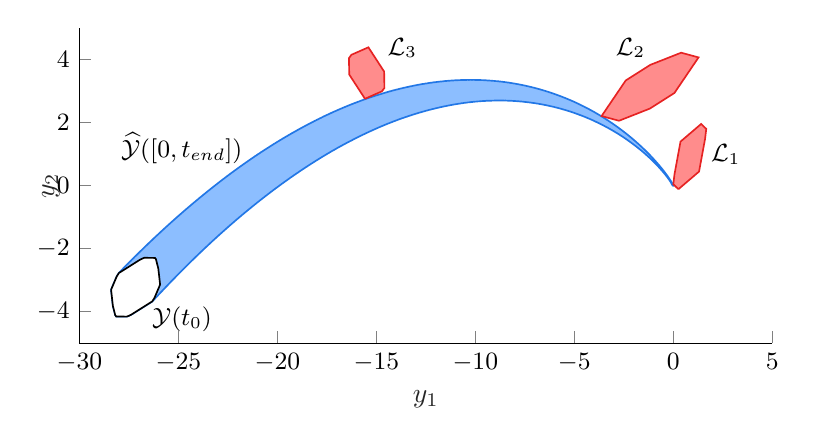
\begin{tikzpicture}[
	every node/.style={font=\small}]

\definecolor{unsafe}{RGB}{255,140,140}			% HSV: 360, 45, 100
\definecolor{unsafeborder}{RGB}{230,34,34}		% HSV: 360, 85, 90
\definecolor{reachouter}{RGB}{140,190,255}		% HSV: 214, 45, 100
\definecolor{reachouterborder}{RGB}{34,119,230}	% HSV: 214, 85, 90

%\draw[red] (-1,-1) grid (13,5.5);
%\draw[red] (10,0) circle(2pt);

% nodes
\node[anchor=west] at (7.9,2.4) {$\mathcal{L}_{1}$};
\node[anchor=south] at (7,3.5) {$\mathcal{L}_{2}$};
\node[anchor=south] at (4.1,3.5) {$\mathcal{L}_{3}$};
\node[anchor=west] at (0.8,0.3) {$\mathcal{Y}(t_0)$};
\node[anchor=south] at (1.3,2.15) {$\widehat{\mathcal{Y}}([0,t_{\text{end}}])$};

\begin{axis}[%
width=8.8cm,
height=4cm,
at={(0,0)},
scale only axis,
xmin=-30.0000,
xmax=5.0000,
xlabel style={font=\color{white!15!black}},
xlabel={$y_1$},
ymin=-5.0000,
ymax=5.0000,
ylabel style={font=\color{white!15!black}, yshift=-15pt},
ylabel={$y_2$},
%axis background/.style={fill=white},
axis x line*=bottom,
axis y line*=left
]

% reachable set
\addplot[semithick,draw=reachouterborder,fill=reachouter, forget plot]
table[row sep=crcr] {%
x	y\\
-27.6085	-4.1574\\
-28.1419	-4.1507\\
-28.1423	-4.1505\\
-28.1904	-4.1084\\
-28.1905	-4.1083\\
-28.3085	-3.8148\\
-28.3088	-3.8137\\
-28.3092	-3.8117\\
-28.3979	-3.3107\\
-28.3979	-3.3105\\
-28.3944	-3.2959\\
-28.3939	-3.2944\\
-28.3937	-3.2937\\
-28.3934	-3.2931\\
-28.3909	-3.2893\\
-28.1132	-2.8791\\
-28.1129	-2.8787\\
-28.0006	-2.7665\\
-27.9994	-2.7653\\
-27.8626	-2.6747\\
-27.8542	-2.6714\\
-27.7225	-2.5848\\
-27.7141	-2.5815\\
-27.5831	-2.4958\\
-27.5748	-2.4926\\
-27.4443	-2.4079\\
-27.436	-2.4048\\
-27.3062	-2.321\\
-27.298	-2.318\\
-27.1688	-2.2352\\
-27.1606	-2.2321\\
-27.032	-2.1503\\
-27.0239	-2.1473\\
-26.8959	-2.0664\\
-26.8878	-2.0635\\
-26.7604	-1.9835\\
-26.7524	-1.9807\\
-26.6256	-1.9016\\
-26.6176	-1.8989\\
-26.4914	-1.8207\\
-26.4835	-1.818\\
-26.3579	-1.7407\\
-26.3501	-1.7381\\
-26.225	-1.6617\\
-26.2172	-1.6591\\
-26.0928	-1.5836\\
-26.085	-1.581\\
-25.9612	-1.5064\\
-25.9535	-1.5039\\
-25.8302	-1.4302\\
-25.8226	-1.4278\\
-25.6999	-1.3549\\
-25.6923	-1.3525\\
-25.5702	-1.2804\\
-25.5626	-1.2781\\
-25.4411	-1.2069\\
-25.4336	-1.2046\\
-25.3126	-1.1343\\
-25.3052	-1.1321\\
-25.1848	-1.0625\\
-25.1774	-1.0604\\
-25.0576	-0.9916\\
-25.0502	-0.9895\\
-24.931	-0.9216\\
-24.9237	-0.9195\\
-24.805	-0.8524\\
-24.7977	-0.8504\\
-24.6796	-0.7841\\
-24.6724	-0.7822\\
-24.5548	-0.7166\\
-24.5476	-0.7147\\
-24.4306	-0.65\\
-24.4235	-0.6481\\
-24.3071	-0.5842\\
-24.3	-0.5823\\
-24.1841	-0.5191\\
-24.1771	-0.5174\\
-24.0617	-0.4549\\
-24.0547	-0.4532\\
-23.9399	-0.3915\\
-23.933	-0.3898\\
-23.8187	-0.3289\\
-23.8118	-0.3272\\
-23.6981	-0.2671\\
-23.6912	-0.2655\\
-23.5781	-0.206\\
-23.5713	-0.2044\\
-23.4586	-0.1457\\
-23.4519	-0.1442\\
-23.3398	-0.0862\\
-23.333	-0.0847\\
-23.2215	-0.0274\\
-23.2148	-0.026\\
-23.1038	0.0306\\
-23.0971	0.032\\
-22.9866	0.0879\\
-22.9821	0.0888\\
-22.841	0.1596\\
-22.8327	0.1613\\
-22.6963	0.2291\\
-22.6881	0.2307\\
-22.5524	0.2974\\
-22.5443	0.2989\\
-22.4094	0.3646\\
-22.4013	0.3661\\
-22.2673	0.4307\\
-22.2593	0.4322\\
-22.126	0.4958\\
-22.1181	0.4972\\
-21.9856	0.5598\\
-21.9777	0.5611\\
-21.8461	0.6227\\
-21.8383	0.624\\
-21.7074	0.6847\\
-21.6996	0.6859\\
-21.5695	0.7455\\
-21.5618	0.7467\\
-21.4325	0.8054\\
-21.4267	0.8063\\
-21.2692	0.877\\
-21.2601	0.8782\\
-21.1071	0.9461\\
-21.098	0.9473\\
-20.9462	1.0138\\
-20.9372	1.0149\\
-20.7864	1.0801\\
-20.7775	1.0812\\
-20.6278	1.1451\\
-20.619	1.1461\\
-20.4704	1.2087\\
-20.4617	1.2096\\
-20.3142	1.271\\
-20.3139	1.271\\
-20.3055	1.2719\\
-20.159	1.332\\
-20.1587	1.3321\\
-20.1504	1.3328\\
-20.0051	1.3918\\
-20.0048	1.3918\\
-19.9965	1.3925\\
-19.8522	1.4502\\
-19.8519	1.4503\\
-19.8437	1.4509\\
-19.7005	1.5075\\
-19.7002	1.5075\\
-19.6921	1.5081\\
-19.5499	1.5635\\
-19.5496	1.5635\\
-19.5415	1.5641\\
-19.4003	1.6183\\
-19.4001	1.6184\\
-19.3921	1.6189\\
-19.2519	1.672\\
-19.2516	1.672\\
-19.2438	1.6724\\
-19.1046	1.7244\\
-19.1043	1.7245\\
-19.0965	1.7249\\
-18.9584	1.7757\\
-18.9581	1.7758\\
-18.9503	1.7761\\
-18.8132	1.8259\\
-18.8129	1.826\\
-18.8052	1.8263\\
-18.6691	1.875\\
-18.6688	1.875\\
-18.6612	1.8753\\
-18.5261	1.923\\
-18.5258	1.923\\
-18.5183	1.9232\\
-18.3841	1.9699\\
-18.3838	1.9699\\
-18.3763	1.9701\\
-18.2432	2.0157\\
-18.2429	2.0157\\
-18.2355	2.0158\\
-18.1033	2.0605\\
-18.103	2.0605\\
-18.0957	2.0606\\
-17.9645	2.1042\\
-17.9642	2.1042\\
-17.9569	2.1043\\
-17.8266	2.1469\\
-17.8264	2.147\\
-17.8214	2.147\\
-17.6445	2.204\\
-17.644	2.204\\
-17.6344	2.2039\\
-17.4641	2.2576\\
-17.4636	2.2577\\
-17.4541	2.2575\\
-17.2855	2.3095\\
-17.285	2.3096\\
-17.2756	2.3094\\
-17.1086	2.3598\\
-17.1082	2.3599\\
-17.0988	2.3596\\
-16.9335	2.4084\\
-16.9331	2.4085\\
-16.9238	2.4081\\
-16.7601	2.4555\\
-16.7597	2.4555\\
-16.7505	2.4551\\
-16.5884	2.5009\\
-16.588	2.501\\
-16.579	2.5005\\
-16.42	2.5444\\
-16.4185	2.5448\\
-16.418	2.5449\\
-16.4091	2.5443\\
-16.2517	2.5868\\
-16.2502	2.5872\\
-16.2497	2.5873\\
-16.2409	2.5867\\
-16.085	2.6278\\
-16.0835	2.6282\\
-16.0831	2.6282\\
-16.0744	2.6275\\
-15.92	2.6673\\
-15.9185	2.6677\\
-15.9181	2.6677\\
-15.9095	2.667\\
-15.7567	2.7054\\
-15.7552	2.7057\\
-15.7548	2.7058\\
-15.7463	2.705\\
-15.5949	2.7421\\
-15.5935	2.7424\\
-15.593	2.7425\\
-15.5847	2.7416\\
-15.4348	2.7774\\
-15.4333	2.7778\\
-15.4329	2.7778\\
-15.4247	2.7769\\
-15.2762	2.8115\\
-15.2748	2.8118\\
-15.2744	2.8118\\
-15.2662	2.8109\\
-15.1192	2.8442\\
-15.1178	2.8445\\
-15.1174	2.8445\\
-15.1093	2.8435\\
-14.9638	2.8757\\
-14.9624	2.8759\\
-14.962	2.876\\
-14.954	2.8749\\
-14.8099	2.9059\\
-14.8085	2.9061\\
-14.8081	2.9062\\
-14.8003	2.9051\\
-14.6576	2.9349\\
-14.6562	2.9351\\
-14.6558	2.9351\\
-14.648	2.934\\
-14.5067	2.9627\\
-14.5054	2.9629\\
-14.5049	2.9629\\
-14.4989	2.962\\
-14.3206	2.997\\
-14.3189	2.9972\\
-14.3184	2.9973\\
-14.3089	2.9958\\
-14.1365	3.0283\\
-14.1348	3.0285\\
-14.1343	3.0286\\
-14.1249	3.027\\
-13.9547	3.0579\\
-13.953	3.0581\\
-13.9524	3.0582\\
-13.9432	3.0566\\
-13.7751	3.0858\\
-13.7734	3.086\\
-13.7729	3.0861\\
-13.7638	3.0844\\
-13.5977	3.1121\\
-13.5956	3.1124\\
-13.5866	3.1106\\
-13.4226	3.1369\\
-13.4221	3.1369\\
-13.4205	3.1371\\
-13.4116	3.1353\\
-13.2497	3.16\\
-13.2491	3.1601\\
-13.2475	3.1602\\
-13.2388	3.1584\\
-13.0789	3.1817\\
-13.0783	3.1818\\
-13.0768	3.1819\\
-13.0696	3.1803\\
-12.877	3.2069\\
-12.8763	3.207\\
-12.8745	3.2071\\
-12.8643	3.2048\\
-12.6779	3.2289\\
-12.6772	3.229\\
-12.6754	3.2291\\
-12.6654	3.2268\\
-12.4818	3.249\\
-12.4811	3.2491\\
-12.4793	3.2492\\
-12.4695	3.2468\\
-12.2886	3.2672\\
-12.2879	3.2673\\
-12.2861	3.2674\\
-12.2765	3.2649\\
-12.0983	3.2836\\
-12.0976	3.2837\\
-12.0958	3.2837\\
-12.0864	3.2812\\
-11.9105	3.2983\\
-11.9084	3.2983\\
-11.8992	3.2958\\
-11.7259	3.3112\\
-11.7238	3.3112\\
-11.7148	3.3087\\
-11.5441	3.3225\\
-11.542	3.3225\\
-11.5332	3.3199\\
-11.3649	3.3322\\
-11.3646	3.3322\\
-11.3629	3.3321\\
-11.3543	3.3295\\
-11.1885	3.3404\\
-11.1869	3.3403\\
-11.1865	3.3403\\
-11.1784	3.3377\\
-11.0651	3.3443\\
-11.0148	3.3471\\
-11.0131	3.347\\
-11.0128	3.347\\
-11.0053	3.3446\\
-10.8933	3.3502\\
-10.8436	3.3524\\
-10.842	3.3522\\
-10.8417	3.3522\\
-10.8348	3.3499\\
-10.724	3.3547\\
-10.6751	3.3563\\
-10.6735	3.3561\\
-10.6732	3.3561\\
-10.6669	3.354\\
-10.5573	3.3578\\
-10.509	3.3589\\
-10.5075	3.3587\\
-10.5072	3.3587\\
-10.5014	3.3567\\
-10.3931	3.3597\\
-10.3455	3.3602\\
-10.344	3.36\\
-10.3437	3.36\\
-10.3385	3.3581\\
-10.2314	3.3603\\
-10.1845	3.3603\\
-10.183	3.3601\\
-10.1827	3.3601\\
-10.1823	3.3599\\
-10.1818	3.3598\\
-10.178	3.3584\\
-10.0722	3.3597\\
-10.0259	3.3592\\
-10.0244	3.359\\
-10.0241	3.359\\
-10.0237	3.3588\\
-10.0233	3.3587\\
-10.0229	3.3585\\
-10.0225	3.3584\\
-10.0221	3.3582\\
-10.0199	3.3574\\
-9.9153	3.358\\
-9.8697	3.357\\
-9.8682	3.3568\\
-9.8679	3.3567\\
-9.8675	3.3566\\
-9.8671	3.3564\\
-9.8667	3.3563\\
-9.8663	3.3561\\
-9.8659	3.356\\
-9.8655	3.3558\\
-9.8651	3.3557\\
-9.8647	3.3555\\
-9.8642	3.3553\\
-9.7608	3.3551\\
-9.7159	3.3537\\
-9.7144	3.3535\\
-9.7141	3.3534\\
-9.7137	3.3533\\
-9.7133	3.3531\\
-9.7129	3.353\\
-9.7125	3.3528\\
-9.7121	3.3527\\
-9.7117	3.3525\\
-9.7113	3.3524\\
-9.7108	3.3522\\
-9.6087	3.3512\\
-9.5644	3.3494\\
-9.5629	3.3492\\
-9.5626	3.3491\\
-9.5622	3.3489\\
-9.5618	3.3488\\
-9.5614	3.3486\\
-9.561	3.3485\\
-9.5606	3.3483\\
-9.5602	3.3482\\
-9.5597	3.348\\
-9.4589	3.3463\\
-9.4152	3.344\\
-9.4137	3.3438\\
-9.4133	3.3436\\
-9.4129	3.3435\\
-9.4125	3.3433\\
-9.4121	3.3432\\
-9.4117	3.343\\
-9.4113	3.3429\\
-9.4109	3.3427\\
-9.3113	3.3404\\
-9.2682	3.3377\\
-9.2668	3.3375\\
-9.2664	3.3373\\
-9.266	3.3372\\
-9.2656	3.337\\
-9.2652	3.3369\\
-9.2648	3.3367\\
-9.2643	3.3366\\
-9.166	3.3336\\
-9.1235	3.3305\\
-9.1221	3.3302\\
-9.1217	3.3301\\
-9.1213	3.3299\\
-9.1209	3.3298\\
-9.1205	3.3296\\
-9.12	3.3295\\
-9.0229	3.3258\\
-8.981	3.3224\\
-8.98	3.3222\\
-8.8358	3.3156\\
-8.7946	3.3117\\
-8.7928	3.3113\\
-8.792	3.3111\\
-8.7916	3.3109\\
-8.7911	3.3108\\
-8.7907	3.3106\\
-8.7903	3.3105\\
-8.7895	3.3101\\
-8.7891	3.31\\
-8.7889	3.3099\\
-8.6525	3.3025\\
-8.6521	3.3025\\
-8.6117	3.2981\\
-8.6099	3.2977\\
-8.6095	3.2976\\
-8.6091	3.2974\\
-8.6087	3.2973\\
-8.6083	3.2971\\
-8.6079	3.297\\
-8.6075	3.2968\\
-8.6071	3.2967\\
-8.6066	3.2965\\
-8.4726	3.2879\\
-8.4722	3.2879\\
-8.4326	3.2831\\
-8.4308	3.2827\\
-8.4304	3.2826\\
-8.43	3.2824\\
-8.4296	3.2823\\
-8.4292	3.2821\\
-8.4288	3.282\\
-8.4284	3.2818\\
-8.4279	3.2816\\
-8.2963	3.2721\\
-8.2959	3.2721\\
-8.257	3.2669\\
-8.2553	3.2664\\
-8.2545	3.2662\\
-8.2541	3.266\\
-8.2537	3.2659\\
-8.2533	3.2657\\
-8.2529	3.2656\\
-8.1235	3.255\\
-8.1232	3.255\\
-8.0851	3.2494\\
-8.0834	3.249\\
-8.0829	3.2488\\
-8.0825	3.2487\\
-8.0821	3.2485\\
-8.0817	3.2484\\
-8.0814	3.2483\\
-7.9543	3.2368\\
-7.954	3.2368\\
-7.9166	3.2308\\
-7.9149	3.2304\\
-7.9145	3.2302\\
-7.9141	3.2301\\
-7.9137	3.2299\\
-7.9135	3.2299\\
-7.7885	3.2175\\
-7.7882	3.2175\\
-7.7515	3.2112\\
-7.7499	3.2107\\
-7.7495	3.2106\\
-7.749	3.2104\\
-7.6261	3.1972\\
-7.6258	3.1971\\
-7.5898	3.1905\\
-7.5882	3.1901\\
-7.5878	3.1899\\
-7.467	3.1759\\
-7.4667	3.1758\\
-7.4314	3.1689\\
-7.43	3.1685\\
-7.3111	3.1537\\
-7.3108	3.1537\\
-7.2762	3.1465\\
-7.2755	3.1463\\
-7.1585	3.1307\\
-7.1581	3.1307\\
-7.1242	3.1232\\
-7.1241	3.1232\\
-7.0089	3.1069\\
-7.0086	3.1069\\
-6.9765	3.0994\\
-6.8624	3.0824\\
-6.8621	3.0823\\
-6.8318	3.075\\
-6.7188	3.0572\\
-6.7185	3.0571\\
-6.69	3.0499\\
-6.579	3.0315\\
-6.5782	3.0314\\
-6.5779	3.0313\\
-6.5512	3.0242\\
-6.4412	3.0051\\
-6.4405	3.005\\
-6.4402	3.0049\\
-6.4151	2.998\\
-6.3063	2.9782\\
-6.3056	2.9781\\
-6.3053	2.978\\
-6.2817	2.9712\\
-6.1742	2.9508\\
-6.1739	2.9508\\
-6.1509	2.9439\\
-6.0447	2.923\\
-6.0444	2.9229\\
-6.0225	2.9161\\
-5.9179	2.8947\\
-5.9177	2.8946\\
-5.8968	2.8879\\
-5.7938	2.8661\\
-5.7935	2.866\\
-5.7735	2.8594\\
-5.6721	2.8371\\
-5.6719	2.837\\
-5.6528	2.8305\\
-5.5554	2.8084\\
-5.553	2.8078\\
-5.5528	2.8078\\
-5.5346	2.8014\\
-5.4387	2.7789\\
-5.4363	2.7783\\
-5.4357	2.7781\\
-5.4218	2.773\\
-5.297	2.7427\\
-5.2941	2.742\\
-5.2937	2.7419\\
-5.2933	2.7417\\
-5.2929	2.7416\\
-5.2925	2.7414\\
-5.2921	2.7413\\
-5.2914	2.741\\
-5.2728	2.734\\
-5.1581	2.7052\\
-5.1553	2.7044\\
-5.1549	2.7043\\
-5.1545	2.7041\\
-5.1541	2.704\\
-5.1537	2.7038\\
-5.1533	2.7037\\
-5.1529	2.7035\\
-5.1525	2.7034\\
-5.1521	2.7032\\
-5.1517	2.7031\\
-5.1513	2.7029\\
-5.1509	2.7028\\
-5.1348	2.6965\\
-5.0228	2.6674\\
-5.0201	2.6666\\
-5.0197	2.6664\\
-5.0193	2.6663\\
-5.0188	2.6661\\
-5.0184	2.666\\
-5.018	2.6658\\
-5.0176	2.6657\\
-5.0172	2.6655\\
-5.0168	2.6654\\
-5.0164	2.6652\\
-5.016	2.6651\\
-5.0157	2.6649\\
-5.0153	2.6648\\
-5.0149	2.6646\\
-5.0145	2.6645\\
-5.0141	2.6643\\
-5.0002	2.6587\\
-4.891	2.6293\\
-4.8883	2.6285\\
-4.8879	2.6284\\
-4.8875	2.6282\\
-4.8871	2.6281\\
-4.8867	2.6279\\
-4.8863	2.6278\\
-4.8859	2.6276\\
-4.8855	2.6275\\
-4.8851	2.6273\\
-4.8847	2.6272\\
-4.8843	2.627\\
-4.8839	2.6269\\
-4.8835	2.6267\\
-4.8831	2.6266\\
-4.8827	2.6264\\
-4.8824	2.6263\\
-4.882	2.6261\\
-4.8816	2.626\\
-4.8808	2.6256\\
-4.8805	2.6255\\
-4.8688	2.6207\\
-4.7626	2.5911\\
-4.76	2.5903\\
-4.7596	2.5902\\
-4.7592	2.59\\
-4.7587	2.5899\\
-4.7583	2.5897\\
-4.7579	2.5896\\
-4.7575	2.5894\\
-4.7571	2.5893\\
-4.7567	2.5891\\
-4.7563	2.589\\
-4.7559	2.5888\\
-4.7555	2.5887\\
-4.7552	2.5885\\
-4.7548	2.5884\\
-4.7544	2.5882\\
-4.754	2.5881\\
-4.7532	2.5877\\
-4.7529	2.5876\\
-4.7525	2.5874\\
-4.7521	2.5873\\
-4.7518	2.5871\\
-4.7514	2.587\\
-4.751	2.5868\\
-4.7507	2.5867\\
-4.7503	2.5865\\
-4.7406	2.5824\\
-4.6375	2.5528\\
-4.6349	2.552\\
-4.6345	2.5518\\
-4.6337	2.5516\\
-4.6333	2.5514\\
-4.6329	2.5513\\
-4.6321	2.5509\\
-4.6317	2.5508\\
-4.6313	2.5506\\
-4.6309	2.5505\\
-4.6305	2.5503\\
-4.6301	2.5502\\
-4.6297	2.55\\
-4.6293	2.5499\\
-4.629	2.5497\\
-4.6286	2.5496\\
-4.6282	2.5494\\
-4.6278	2.5493\\
-4.6275	2.5491\\
-4.6271	2.549\\
-4.6267	2.5488\\
-4.6263	2.5487\\
-4.626	2.5485\\
-4.6256	2.5484\\
-4.6252	2.5482\\
-4.6249	2.5481\\
-4.6245	2.5479\\
-4.6242	2.5478\\
-4.6238	2.5476\\
-4.6235	2.5474\\
-4.6156	2.544\\
-4.5156	2.5145\\
-4.5131	2.5136\\
-4.5127	2.5135\\
-4.5123	2.5133\\
-4.5119	2.5132\\
-4.5115	2.513\\
-4.5111	2.5129\\
-4.5107	2.5127\\
-4.5103	2.5126\\
-4.5099	2.5124\\
-4.5095	2.5123\\
-4.5091	2.5121\\
-4.5087	2.512\\
-4.5083	2.5118\\
-4.5079	2.5117\\
-4.5075	2.5115\\
-4.5072	2.5114\\
-4.5068	2.5112\\
-4.5064	2.5111\\
-4.506	2.5109\\
-4.5056	2.5108\\
-4.5053	2.5106\\
-4.5049	2.5104\\
-4.5045	2.5103\\
-4.5042	2.5101\\
-4.5038	2.51\\
-4.5034	2.5098\\
-4.5031	2.5097\\
-4.5027	2.5095\\
-4.5024	2.5094\\
-4.502	2.5092\\
-4.5017	2.5091\\
-4.5013	2.5089\\
-4.501	2.5088\\
-4.5006	2.5086\\
-4.5003	2.5085\\
-4.4999	2.5083\\
-4.4937	2.5055\\
-4.3969	2.4761\\
-4.3941	2.4751\\
-4.3936	2.4749\\
-4.3932	2.4748\\
-4.3928	2.4746\\
-4.3924	2.4745\\
-4.392	2.4743\\
-4.3916	2.4742\\
-4.3912	2.474\\
-4.3908	2.4739\\
-4.3904	2.4737\\
-4.39	2.4736\\
-4.3896	2.4734\\
-4.3893	2.4733\\
-4.3889	2.4731\\
-4.3885	2.473\\
-4.3881	2.4728\\
-4.3877	2.4727\\
-4.3874	2.4725\\
-4.387	2.4724\\
-4.3862	2.472\\
-4.3859	2.4719\\
-4.3855	2.4717\\
-4.3851	2.4716\\
-4.3848	2.4714\\
-4.3844	2.4713\\
-4.3841	2.4711\\
-4.3837	2.471\\
-4.3833	2.4708\\
-4.383	2.4707\\
-4.3826	2.4705\\
-4.3823	2.4704\\
-4.3819	2.4702\\
-4.3816	2.4701\\
-4.3813	2.4699\\
-4.3809	2.4698\\
-4.3806	2.4696\\
-4.3802	2.4694\\
-4.3799	2.4693\\
-4.3795	2.4691\\
-4.377	2.468\\
-4.2591	2.4311\\
-4.2587	2.4309\\
-4.2583	2.4308\\
-4.2579	2.4306\\
-4.2575	2.4305\\
-4.2571	2.4303\\
-4.2567	2.4302\\
-4.2535	2.429\\
-4.2527	2.4286\\
-4.2523	2.4285\\
-4.2519	2.4283\\
-4.2515	2.4282\\
-4.2511	2.428\\
-4.2507	2.4279\\
-4.2503	2.4277\\
-4.2499	2.4276\\
-4.2496	2.4274\\
-4.2492	2.4273\\
-4.2488	2.4271\\
-4.2484	2.427\\
-4.2481	2.4268\\
-4.2477	2.4267\\
-4.2473	2.4265\\
-4.247	2.4264\\
-4.2466	2.4262\\
-4.2463	2.4261\\
-4.2459	2.4259\\
-4.2455	2.4258\\
-4.2452	2.4256\\
-4.2448	2.4254\\
-4.2445	2.4253\\
-4.2441	2.4251\\
-4.2438	2.425\\
-4.2434	2.4248\\
-4.2431	2.4247\\
-4.2428	2.4245\\
-4.2424	2.4244\\
-4.2421	2.4242\\
-4.2418	2.4241\\
-4.2413	2.4239\\
-4.2397	2.4231\\
-4.2331	2.42\\
-4.125	2.3851\\
-4.1246	2.3849\\
-4.1241	2.3848\\
-4.1237	2.3846\\
-4.1233	2.3845\\
-4.1229	2.3843\\
-4.1225	2.3842\\
-4.1221	2.384\\
-4.1217	2.3839\\
-4.1213	2.3837\\
-4.1209	2.3836\\
-4.1205	2.3834\\
-4.1202	2.3833\\
-4.1198	2.3831\\
-4.117	2.382\\
-4.1166	2.3819\\
-4.1163	2.3817\\
-4.1159	2.3816\\
-4.1155	2.3814\\
-4.1151	2.3813\\
-4.1147	2.3811\\
-4.1144	2.381\\
-4.114	2.3808\\
-4.1136	2.3807\\
-4.1133	2.3805\\
-4.1129	2.3804\\
-4.1125	2.3802\\
-4.1122	2.3801\\
-4.1118	2.3799\\
-4.1115	2.3798\\
-4.1111	2.3796\\
-4.1108	2.3795\\
-4.1104	2.3793\\
-4.1101	2.3791\\
-4.1097	2.379\\
-4.1094	2.3788\\
-4.109	2.3787\\
-4.1087	2.3785\\
-4.1084	2.3784\\
-4.108	2.3782\\
-4.1077	2.3781\\
-4.1069	2.3777\\
-4.1064	2.3775\\
-4.1048	2.3767\\
-4.1044	2.3766\\
-4.0986	2.3737\\
-3.995	2.3392\\
-3.9946	2.3391\\
-3.9942	2.3389\\
-3.9937	2.3388\\
-3.9933	2.3386\\
-3.9929	2.3385\\
-3.9925	2.3383\\
-3.9921	2.3382\\
-3.9917	2.338\\
-3.9913	2.3379\\
-3.9909	2.3377\\
-3.9906	2.3376\\
-3.9902	2.3374\\
-3.9898	2.3373\\
-3.9894	2.3371\\
-3.989	2.337\\
-3.9886	2.3368\\
-3.9882	2.3367\\
-3.9879	2.3365\\
-3.9875	2.3364\\
-3.9845	2.3351\\
-3.9841	2.335\\
-3.9837	2.3348\\
-3.9834	2.3347\\
-3.983	2.3345\\
-3.9826	2.3344\\
-3.9823	2.3342\\
-3.9819	2.3341\\
-3.9816	2.3339\\
-3.9812	2.3338\\
-3.9809	2.3336\\
-3.9805	2.3335\\
-3.9802	2.3333\\
-3.9798	2.3331\\
-3.9795	2.333\\
-3.9791	2.3328\\
-3.9788	2.3327\\
-3.9784	2.3325\\
-3.9781	2.3324\\
-3.9778	2.3322\\
-3.9774	2.332\\
-3.9769	2.3318\\
-3.9765	2.3317\\
-3.9737	2.3303\\
-3.9734	2.3301\\
-3.9724	2.3297\\
-3.972	2.3294\\
-3.9689	2.3279\\
-3.8689	2.2937\\
-3.8685	2.2935\\
-3.8681	2.2934\\
-3.8676	2.2932\\
-3.8672	2.2931\\
-3.8668	2.2929\\
-3.8664	2.2928\\
-3.866	2.2926\\
-3.8656	2.2925\\
-3.8652	2.2923\\
-3.8648	2.2922\\
-3.8645	2.292\\
-3.8641	2.2918\\
-3.8637	2.2917\\
-3.8633	2.2915\\
-3.8629	2.2914\\
-3.8625	2.2912\\
-3.8621	2.2911\\
-3.8618	2.2909\\
-3.8614	2.2908\\
-3.861	2.2906\\
-3.8607	2.2905\\
-3.8603	2.2903\\
-3.8599	2.2902\\
-3.8596	2.29\\
-3.8592	2.2899\\
-3.8563	2.2886\\
-3.8559	2.2885\\
-3.8555	2.2883\\
-3.8552	2.2882\\
-3.8548	2.288\\
-3.8545	2.2879\\
-3.8541	2.2877\\
-3.8538	2.2875\\
-3.8534	2.2874\\
-3.8531	2.2872\\
-3.8528	2.2871\\
-3.8524	2.2869\\
-3.8521	2.2868\\
-3.8518	2.2866\\
-3.8513	2.2864\\
-3.8509	2.2862\\
-3.8505	2.2861\\
-3.8469	2.2843\\
-3.8464	2.2841\\
-3.846	2.2839\\
-3.8455	2.2836\\
-3.8451	2.2834\\
-3.8446	2.2832\\
-3.8442	2.2829\\
-3.8414	2.2815\\
-3.7469	2.2482\\
-3.7464	2.2481\\
-3.746	2.2479\\
-3.7452	2.2477\\
-3.7444	2.2473\\
-3.744	2.2472\\
-3.7436	2.247\\
-3.7432	2.2469\\
-3.7428	2.2467\\
-3.7424	2.2466\\
-3.742	2.2464\\
-3.7416	2.2463\\
-3.7413	2.2461\\
-3.7409	2.246\\
-3.7405	2.2458\\
-3.7401	2.2457\\
-3.7397	2.2455\\
-3.7394	2.2454\\
-3.739	2.2452\\
-3.7386	2.2451\\
-3.7383	2.2449\\
-3.7379	2.2448\\
-3.7375	2.2446\\
-3.7372	2.2445\\
-3.7368	2.2443\\
-3.7364	2.2442\\
-3.7361	2.244\\
-3.7357	2.2439\\
-3.7354	2.2437\\
-3.735	2.2435\\
-3.7347	2.2434\\
-3.7318	2.2421\\
-3.7315	2.242\\
-3.7311	2.2418\\
-3.7308	2.2417\\
-3.7305	2.2415\\
-3.7301	2.2414\\
-3.7298	2.2412\\
-3.7286	2.2406\\
-3.7282	2.2405\\
-3.7277	2.2403\\
-3.7265	2.2397\\
-3.7262	2.2395\\
-3.7254	2.2391\\
-3.7249	2.2389\\
-3.7245	2.2387\\
-3.724	2.2384\\
-3.7236	2.2382\\
-3.7231	2.238\\
-3.7227	2.2378\\
-3.7222	2.2375\\
-3.7214	2.2371\\
-3.7209	2.2369\\
-3.7187	2.2357\\
-3.6282	2.203\\
-3.6278	2.2028\\
-3.6274	2.2027\\
-3.627	2.2025\\
-3.6266	2.2024\\
-3.6262	2.2022\\
-3.6258	2.2021\\
-3.6254	2.2019\\
-3.625	2.2018\\
-3.6246	2.2016\\
-3.6242	2.2015\\
-3.6238	2.2013\\
-3.6234	2.2012\\
-3.623	2.201\\
-3.6226	2.2009\\
-3.6223	2.2007\\
-3.6219	2.2006\\
-3.6215	2.2004\\
-3.6211	2.2003\\
-3.6208	2.2001\\
-3.6204	2.2\\
-3.62	2.1998\\
-3.6197	2.1996\\
-3.6193	2.1995\\
-3.6189	2.1993\\
-3.6186	2.1992\\
-3.6182	2.199\\
-3.6179	2.1989\\
-3.6175	2.1987\\
-3.6171	2.1986\\
-3.6168	2.1984\\
-3.6164	2.1983\\
-3.6161	2.1981\\
-3.6158	2.198\\
-3.6154	2.1978\\
-3.6151	2.1977\\
-3.6147	2.1975\\
-3.6144	2.1974\\
-3.6116	2.1961\\
-3.6092	2.1949\\
-3.6088	2.1948\\
-3.6068	2.1938\\
-3.6063	2.1935\\
-3.6058	2.1933\\
-3.6054	2.1931\\
-3.6049	2.1929\\
-3.6045	2.1926\\
-3.6041	2.1924\\
-3.6036	2.1922\\
-3.6032	2.192\\
-3.6028	2.1917\\
-3.6023	2.1915\\
-3.6015	2.1911\\
-3.6011	2.1908\\
-3.5997	2.1901\\
-3.512	2.1576\\
-3.5116	2.1574\\
-3.5112	2.1573\\
-3.5108	2.1571\\
-3.5104	2.157\\
-3.51	2.1568\\
-3.5096	2.1567\\
-3.5092	2.1565\\
-3.5089	2.1564\\
-3.5085	2.1562\\
-3.5081	2.1561\\
-3.5077	2.1559\\
-3.5073	2.1558\\
-3.507	2.1556\\
-3.5066	2.1555\\
-3.5062	2.1553\\
-3.5058	2.1552\\
-3.5055	2.155\\
-3.5051	2.1549\\
-3.5047	2.1547\\
-3.5044	2.1545\\
-3.504	2.1544\\
-3.5037	2.1542\\
-3.5033	2.1541\\
-3.5029	2.1539\\
-3.5026	2.1538\\
-3.5022	2.1536\\
-3.5019	2.1535\\
-3.5016	2.1533\\
-3.5012	2.1532\\
-3.5009	2.153\\
-3.5005	2.1529\\
-3.5002	2.1527\\
-3.4998	2.1526\\
-3.4995	2.1524\\
-3.4975	2.1514\\
-3.4951	2.1503\\
-3.4947	2.1501\\
-3.4943	2.15\\
-3.4923	2.149\\
-3.4918	2.1487\\
-3.4914	2.1485\\
-3.4909	2.1483\\
-3.4905	2.1481\\
-3.49	2.1478\\
-3.4896	2.1476\\
-3.4891	2.1474\\
-3.4887	2.1472\\
-3.4883	2.1469\\
-3.4879	2.1467\\
-3.4874	2.1465\\
-3.487	2.1463\\
-3.4866	2.146\\
-3.485	2.1452\\
-3.4843	2.1448\\
-3.3998	2.1127\\
-3.3994	2.1126\\
-3.3991	2.1124\\
-3.3987	2.1122\\
-3.3983	2.1121\\
-3.3979	2.1119\\
-3.3975	2.1118\\
-3.3971	2.1116\\
-3.3967	2.1115\\
-3.3964	2.1113\\
-3.396	2.1112\\
-3.3956	2.111\\
-3.3952	2.1109\\
-3.3949	2.1107\\
-3.3945	2.1106\\
-3.3941	2.1104\\
-3.3938	2.1103\\
-3.3934	2.1101\\
-3.393	2.11\\
-3.3927	2.1098\\
-3.3923	2.1097\\
-3.392	2.1095\\
-3.3916	2.1094\\
-3.3913	2.1092\\
-3.3909	2.109\\
-3.3906	2.1089\\
-3.3902	2.1087\\
-3.3899	2.1086\\
-3.3895	2.1084\\
-3.3892	2.1083\\
-3.3889	2.1081\\
-3.3885	2.108\\
-3.3853	2.1064\\
-3.3849	2.1063\\
-3.3845	2.1061\\
-3.3822	2.105\\
-3.3818	2.1048\\
-3.3814	2.1045\\
-3.3809	2.1043\\
-3.3805	2.1041\\
-3.38	2.1039\\
-3.3796	2.1036\\
-3.3791	2.1034\\
-3.3787	2.1032\\
-3.3782	2.103\\
-3.3778	2.1027\\
-3.377	2.1023\\
-3.3765	2.1021\\
-3.3761	2.1018\\
-3.3749	2.1012\\
-3.3745	2.1009\\
-3.3729	2.1001\\
-3.3726	2.0999\\
-3.2908	2.0681\\
-3.2904	2.0679\\
-3.29	2.0678\\
-3.2896	2.0676\\
-3.2892	2.0675\\
-3.2888	2.0673\\
-3.2885	2.0672\\
-3.2881	2.067\\
-3.2877	2.0669\\
-3.2874	2.0667\\
-3.287	2.0665\\
-3.2866	2.0664\\
-3.2863	2.0662\\
-3.2859	2.0661\\
-3.2855	2.0659\\
-3.2852	2.0658\\
-3.2848	2.0656\\
-3.2845	2.0655\\
-3.2841	2.0653\\
-3.2838	2.0652\\
-3.2834	2.065\\
-3.2831	2.0649\\
-3.2827	2.0647\\
-3.2824	2.0646\\
-3.282	2.0644\\
-3.2817	2.0642\\
-3.2814	2.0641\\
-3.281	2.0639\\
-3.2806	2.0638\\
-3.2766	2.0618\\
-3.2761	2.0616\\
-3.2757	2.0614\\
-3.2752	2.0612\\
-3.2726	2.0598\\
-3.2721	2.0596\\
-3.2717	2.0594\\
-3.2712	2.0591\\
-3.2704	2.0587\\
-3.2699	2.0585\\
-3.2695	2.0582\\
-3.2683	2.0576\\
-3.2678	2.0574\\
-3.2674	2.0571\\
-3.2658	2.0563\\
-3.2655	2.056\\
-3.2643	2.0554\\
-3.1855	2.024\\
-3.1851	2.0239\\
-3.1847	2.0237\\
-3.1843	2.0236\\
-3.1839	2.0234\\
-3.1836	2.0232\\
-3.1832	2.0231\\
-3.1828	2.0229\\
-3.1825	2.0228\\
-3.1821	2.0226\\
-3.1817	2.0225\\
-3.1814	2.0223\\
-3.181	2.0222\\
-3.1807	2.022\\
-3.1803	2.0219\\
-3.18	2.0217\\
-3.1796	2.0216\\
-3.1793	2.0214\\
-3.1789	2.0213\\
-3.1786	2.0211\\
-3.1782	2.021\\
-3.1779	2.0208\\
-3.1775	2.0206\\
-3.1772	2.0205\\
-3.1769	2.0203\\
-3.1765	2.0202\\
-3.176	2.02\\
-3.1728	2.0184\\
-3.1725	2.0182\\
-3.1715	2.0178\\
-3.1711	2.0176\\
-3.1706	2.0173\\
-3.1702	2.0171\\
-3.1697	2.0169\\
-3.1693	2.0167\\
-3.1689	2.0164\\
-3.1659	2.0149\\
-3.1654	2.0146\\
-3.1638	2.0138\\
-3.1634	2.0135\\
-3.1618	2.0127\\
-3.1614	2.0124\\
-3.1602	2.0118\\
-3.1597	2.0115\\
-3.1594	2.0113\\
-3.0831	1.9803\\
-3.0827	1.9801\\
-3.0823	1.98\\
-3.0819	1.9798\\
-3.0816	1.9796\\
-3.0812	1.9795\\
-3.0809	1.9793\\
-3.0805	1.9792\\
-3.0801	1.979\\
-3.0798	1.9789\\
-3.0794	1.9787\\
-3.0791	1.9786\\
-3.0787	1.9784\\
-3.0784	1.9783\\
-3.078	1.9781\\
-3.0777	1.978\\
-3.0773	1.9778\\
-3.077	1.9777\\
-3.0767	1.9775\\
-3.0763	1.9774\\
-3.076	1.9772\\
-3.0752	1.9768\\
-3.0747	1.9766\\
-3.0739	1.9762\\
-3.0735	1.9761\\
-3.0723	1.9755\\
-3.072	1.9753\\
-3.0716	1.9751\\
-3.0711	1.9749\\
-3.0706	1.9746\\
-3.0702	1.9744\\
-3.0697	1.9742\\
-3.0693	1.974\\
-3.0688	1.9737\\
-3.068	1.9733\\
-3.0675	1.9731\\
-3.0671	1.9728\\
-3.0663	1.9724\\
-3.0642	1.9713\\
-3.0638	1.9711\\
-3.0634	1.9708\\
-3.0629	1.9706\\
-3.0617	1.97\\
-3.0613	1.9697\\
-3.0605	1.9693\\
-3.0602	1.9691\\
-3.0598	1.9689\\
-3.0594	1.9686\\
-3.0589	1.9684\\
-3.0579	1.9678\\
-3.0578	1.9677\\
-2.9842	1.9371\\
-2.9838	1.937\\
-2.9835	1.9368\\
-2.9831	1.9367\\
-2.9828	1.9365\\
-2.9824	1.9364\\
-2.982	1.9362\\
-2.9817	1.9361\\
-2.9813	1.9359\\
-2.981	1.9358\\
-2.9806	1.9356\\
-2.9803	1.9355\\
-2.98	1.9353\\
-2.9796	1.9352\\
-2.9793	1.935\\
-2.9789	1.9348\\
-2.9786	1.9347\\
-2.9783	1.9345\\
-2.9778	1.9343\\
-2.9774	1.9342\\
-2.9734	1.9322\\
-2.9729	1.932\\
-2.9725	1.9318\\
-2.972	1.9315\\
-2.9716	1.9313\\
-2.9711	1.9311\\
-2.9707	1.9309\\
-2.9702	1.9306\\
-2.969	1.93\\
-2.9685	1.9297\\
-2.9673	1.9291\\
-2.9669	1.9288\\
-2.9645	1.9275\\
-2.9633	1.9269\\
-2.9629	1.9266\\
-2.9617	1.926\\
-2.9597	1.9248\\
-2.9593	1.9246\\
-2.8881	1.8944\\
-2.8877	1.8942\\
-2.8874	1.8941\\
-2.887	1.8939\\
-2.8867	1.8938\\
-2.8863	1.8936\\
-2.886	1.8935\\
-2.8856	1.8933\\
-2.8853	1.8932\\
-2.8849	1.893\\
-2.8846	1.8928\\
-2.8843	1.8927\\
-2.8839	1.8925\\
-2.8836	1.8924\\
-2.8824	1.8918\\
-2.8819	1.8916\\
-2.8811	1.8912\\
-2.8807	1.8911\\
-2.8803	1.8909\\
-2.88	1.8907\\
-2.8792	1.8903\\
-2.8787	1.8901\\
-2.8783	1.8898\\
-2.8773	1.8894\\
-2.8769	1.8892\\
-2.8765	1.8889\\
-2.876	1.8887\\
-2.8756	1.8885\\
-2.8751	1.8883\\
-2.8747	1.888\\
-2.8735	1.8874\\
-2.873	1.8871\\
-2.8714	1.8863\\
-2.871	1.886\\
-2.8706	1.8858\\
-2.8683	1.8845\\
-2.8675	1.8841\\
-2.8671	1.8838\\
-2.8666	1.8836\\
-2.8651	1.8827\\
-2.8647	1.8824\\
-2.8642	1.8821\\
-2.864	1.882\\
-2.7953	1.8523\\
-2.795	1.8521\\
-2.7946	1.852\\
-2.7943	1.8518\\
-2.7939	1.8517\\
-2.7936	1.8515\\
-2.7932	1.8514\\
-2.7929	1.8512\\
-2.7926	1.8511\\
-2.7922	1.8509\\
-2.7919	1.8508\\
-2.7903	1.85\\
-2.7898	1.8498\\
-2.7886	1.8492\\
-2.7883	1.849\\
-2.7879	1.8489\\
-2.7875	1.8487\\
-2.787	1.8484\\
-2.7866	1.8482\\
-2.7861	1.848\\
-2.7857	1.8478\\
-2.7852	1.8475\\
-2.7848	1.8473\\
-2.7843	1.8471\\
-2.7839	1.8469\\
-2.7835	1.8466\\
-2.783	1.8464\\
-2.7822	1.846\\
-2.7818	1.8457\\
-2.7813	1.8455\\
-2.7801	1.8449\\
-2.7797	1.8446\\
-2.7785	1.844\\
-2.7782	1.8438\\
-2.7778	1.8435\\
-2.7774	1.8433\\
-2.7769	1.843\\
-2.775	1.8419\\
-2.7745	1.8417\\
-2.7725	1.8405\\
-2.7721	1.8402\\
-2.7716	1.8399\\
-2.7055	1.8108\\
-2.7051	1.8106\\
-2.7048	1.8105\\
-2.7044	1.8103\\
-2.7041	1.8101\\
-2.7038	1.81\\
-2.7034	1.8098\\
-2.7031	1.8097\\
-2.7023	1.8093\\
-2.7018	1.8091\\
-2.7006	1.8085\\
-2.7002	1.8084\\
-2.6994	1.808\\
-2.6991	1.8078\\
-2.6987	1.8076\\
-2.6982	1.8074\\
-2.6977	1.8071\\
-2.6973	1.8069\\
-2.6968	1.8067\\
-2.6964	1.8065\\
-2.6959	1.8062\\
-2.6951	1.8058\\
-2.6946	1.8056\\
-2.6942	1.8053\\
-2.6934	1.8049\\
-2.6929	1.8047\\
-2.6925	1.8044\\
-2.6909	1.8036\\
-2.6905	1.8033\\
-2.6893	1.8027\\
-2.689	1.8025\\
-2.6886	1.8022\\
-2.6881	1.802\\
-2.6866	1.8011\\
-2.6848	1.8\\
-2.6838	1.7994\\
-2.6833	1.7992\\
-2.6829	1.7989\\
-2.6824	1.7986\\
-2.6821	1.7984\\
-2.6181	1.7696\\
-2.6177	1.7695\\
-2.6174	1.7693\\
-2.6171	1.7692\\
-2.6167	1.769\\
-2.6162	1.7688\\
-2.6142	1.7678\\
-2.6138	1.7677\\
-2.6122	1.7669\\
-2.6117	1.7666\\
-2.6113	1.7664\\
-2.6108	1.7662\\
-2.6104	1.7659\\
-2.6099	1.7657\\
-2.6091	1.7653\\
-2.6086	1.765\\
-2.6078	1.7646\\
-2.6073	1.7644\\
-2.6069	1.7641\\
-2.6053	1.7633\\
-2.6049	1.763\\
-2.6033	1.7622\\
-2.6029	1.7619\\
-2.6026	1.7617\\
-2.6021	1.7614\\
-2.6016	1.7612\\
-2.5996	1.76\\
-2.5992	1.7597\\
-2.5069	1.7174\\
-2.5041	1.716\\
-2.5037	1.7159\\
-2.5025	1.7153\\
-2.502	1.715\\
-2.5015	1.7148\\
-2.5011	1.7146\\
-2.5006	1.7143\\
-2.4998	1.7139\\
-2.4993	1.7137\\
-2.4989	1.7134\\
-2.4985	1.7132\\
-2.498	1.713\\
-2.4976	1.7128\\
-2.4972	1.7125\\
-2.4956	1.7117\\
-2.4952	1.7114\\
-2.4936	1.7106\\
-2.4932	1.7103\\
-2.4928	1.7101\\
-2.4918	1.7095\\
-2.4913	1.7093\\
-2.4908	1.709\\
-2.4904	1.7087\\
-2.4889	1.7078\\
-2.4885	1.7076\\
-2.488	1.7073\\
-2.4876	1.707\\
-2.4853	1.7056\\
-2.4848	1.7053\\
-2.4844	1.705\\
-2.484	1.7048\\
-2.4835	1.7045\\
-2.4831	1.7042\\
-2.4827	1.704\\
-2.4819	1.7034\\
-2.4815	1.7032\\
-2.4811	1.7029\\
-2.3998	1.6647\\
-2.3982	1.6639\\
-2.3978	1.6638\\
-2.397	1.6634\\
-2.3965	1.6631\\
-2.3961	1.6629\\
-2.3956	1.6627\\
-2.3952	1.6625\\
-2.3947	1.6622\\
-2.3939	1.6618\\
-2.3934	1.6616\\
-2.393	1.6613\\
-2.3926	1.6611\\
-2.3921	1.6609\\
-2.3917	1.6607\\
-2.3913	1.6604\\
-2.3897	1.6596\\
-2.3893	1.6593\\
-2.3877	1.6585\\
-2.3873	1.6582\\
-2.3869	1.658\\
-2.3859	1.6574\\
-2.3854	1.6572\\
-2.3849	1.6569\\
-2.3845	1.6566\\
-2.383	1.6557\\
-2.3826	1.6555\\
-2.3821	1.6552\\
-2.3817	1.6549\\
-2.3812	1.6546\\
-2.3808	1.6544\\
-2.3804	1.6541\\
-2.3799	1.6538\\
-2.3773	1.6521\\
-2.3769	1.6519\\
-2.3765	1.6516\\
-2.376	1.6513\\
-2.3756	1.6511\\
-2.3751	1.6507\\
-2.3746	1.6504\\
-2.3745	1.6503\\
-2.2967	1.6129\\
-2.2951	1.6121\\
-2.2946	1.6119\\
-2.2942	1.6117\\
-2.2937	1.6114\\
-2.2933	1.6112\\
-2.2928	1.611\\
-2.2924	1.6108\\
-2.2919	1.6105\\
-2.2907	1.6099\\
-2.2902	1.6096\\
-2.2886	1.6088\\
-2.2882	1.6085\\
-2.2866	1.6077\\
-2.2862	1.6074\\
-2.2854	1.607\\
-2.2844	1.6064\\
-2.284	1.6061\\
-2.2835	1.6058\\
-2.283	1.6056\\
-2.282	1.605\\
-2.2816	1.6047\\
-2.2811	1.6044\\
-2.2807	1.6042\\
-2.2802	1.6039\\
-2.2798	1.6036\\
-2.2793	1.6033\\
-2.2789	1.6031\\
-2.2785	1.6028\\
-2.278	1.6025\\
-2.2776	1.6022\\
-2.2772	1.602\\
-2.2764	1.6014\\
-2.2743	1.6001\\
-2.2738	1.5997\\
-2.2723	1.5988\\
-2.1983	1.5624\\
-2.1979	1.5622\\
-2.1974	1.562\\
-2.1969	1.5617\\
-2.1965	1.5615\\
-2.196	1.5613\\
-2.1956	1.5611\\
-2.1952	1.5608\\
-2.1947	1.5606\\
-2.1939	1.5602\\
-2.1934	1.5599\\
-2.1922	1.5593\\
-2.1918	1.559\\
-2.1902	1.5582\\
-2.1898	1.5579\\
-2.1882	1.5571\\
-2.1862	1.5559\\
-2.1858	1.5556\\
-2.1853	1.5554\\
-2.1848	1.5551\\
-2.1844	1.5548\\
-2.1834	1.5542\\
-2.183	1.554\\
-2.1825	1.5537\\
-2.1817	1.5531\\
-2.1812	1.5529\\
-2.1804	1.5523\\
-2.18	1.5521\\
-2.1792	1.5515\\
-2.1782	1.5509\\
-2.1777	1.5505\\
-2.1752	1.5489\\
-2.1747	1.5485\\
-2.1744	1.5484\\
-2.1038	1.5129\\
-2.1034	1.5127\\
-2.1029	1.5125\\
-2.1025	1.5122\\
-2.102	1.512\\
-2.1012	1.5116\\
-2.1007	1.5113\\
-2.0995	1.5107\\
-2.099	1.5105\\
-2.0986	1.5102\\
-2.097	1.5094\\
-2.0966	1.5091\\
-2.0962	1.5089\\
-2.0959	1.5087\\
-2.0951	1.5083\\
-2.0926	1.5068\\
-2.0922	1.5065\\
-2.0917	1.5063\\
-2.0912	1.506\\
-2.0908	1.5057\\
-2.0903	1.5054\\
-2.0899	1.5051\\
-2.0894	1.5049\\
-2.089	1.5046\\
-2.0885	1.5043\\
-2.0881	1.504\\
-2.0877	1.5038\\
-2.0873	1.5035\\
-2.0868	1.5032\\
-2.0864	1.503\\
-2.086	1.5027\\
-2.085	1.5021\\
-2.0845	1.5017\\
-2.0841	1.5014\\
-2.0831	1.5008\\
-2.0826	1.5004\\
-2.0806	1.4991\\
-2.0132	1.4646\\
-2.0128	1.4643\\
-2.0124	1.4641\\
-2.0119	1.4639\\
-2.0115	1.4637\\
-2.0111	1.4634\\
-2.0107	1.4632\\
-2.0102	1.463\\
-2.0098	1.4628\\
-2.0094	1.4625\\
-2.0078	1.4617\\
-2.0074	1.4614\\
-2.0062	1.4608\\
-2.0059	1.4606\\
-2.0034	1.4591\\
-2.0029	1.4589\\
-2.0025	1.4586\\
-2.0015	1.458\\
-2.0011	1.4577\\
-2.0006	1.4575\\
-2.0002	1.4572\\
-1.9997	1.4569\\
-1.9993	1.4566\\
-1.9989	1.4564\\
-1.9985	1.4561\\
-1.998	1.4558\\
-1.9976	1.4556\\
-1.9968	1.455\\
-1.9958	1.4544\\
-1.9953	1.454\\
-1.9948	1.4537\\
-1.9944	1.4534\\
-1.9934	1.4528\\
-1.993	1.4524\\
-1.9924	1.4521\\
-1.9919	1.4517\\
-1.9907	1.4509\\
-1.9265	1.4173\\
-1.926	1.4171\\
-1.9252	1.4167\\
-1.9248	1.4164\\
-1.9244	1.4162\\
-1.9239	1.416\\
-1.9235	1.4158\\
-1.9231	1.4155\\
-1.9219	1.4149\\
-1.9216	1.4147\\
-1.9212	1.4144\\
-1.9204	1.414\\
-1.9194	1.4134\\
-1.9189	1.4132\\
-1.9179	1.4126\\
-1.9175	1.4123\\
-1.9165	1.4117\\
-1.9161	1.4115\\
-1.9156	1.4112\\
-1.9152	1.4109\\
-1.9147	1.4106\\
-1.9143	1.4104\\
-1.9138	1.4101\\
-1.913	1.4095\\
-1.9126	1.4093\\
-1.9121	1.409\\
-1.9117	1.4087\\
-1.9113	1.4085\\
-1.9108	1.4081\\
-1.9098	1.4075\\
-1.9094	1.4072\\
-1.9089	1.4068\\
-1.9084	1.4065\\
-1.908	1.4062\\
-1.9075	1.4059\\
-1.907	1.4055\\
-1.9064	1.4051\\
-1.9059	1.4048\\
-1.9054	1.4044\\
-1.9049	1.4041\\
-1.9046	1.4038\\
-1.8433	1.3712\\
-1.8421	1.3706\\
-1.8417	1.3703\\
-1.8401	1.3695\\
-1.8397	1.3692\\
-1.8385	1.3686\\
-1.837	1.3677\\
-1.8366	1.3674\\
-1.8361	1.3672\\
-1.8351	1.3666\\
-1.8347	1.3663\\
-1.8342	1.366\\
-1.8337	1.3658\\
-1.8333	1.3655\\
-1.8328	1.3652\\
-1.8324	1.3649\\
-1.832	1.3647\\
-1.8315	1.3644\\
-1.8307	1.3638\\
-1.8303	1.3636\\
-1.8295	1.363\\
-1.828	1.3621\\
-1.8275	1.3617\\
-1.827	1.3614\\
-1.8266	1.3611\\
-1.8256	1.3605\\
-1.8246	1.3597\\
-1.824	1.3594\\
-1.823	1.3586\\
-1.8225	1.3583\\
-1.822	1.3579\\
-1.7637	1.3263\\
-1.7633	1.3261\\
-1.7629	1.3258\\
-1.7613	1.325\\
-1.7609	1.3247\\
-1.7601	1.3243\\
-1.7586	1.3234\\
-1.7581	1.3232\\
-1.7577	1.3229\\
-1.7562	1.322\\
-1.7558	1.3217\\
-1.7553	1.3215\\
-1.7549	1.3212\\
-1.7544	1.3209\\
-1.754	1.3206\\
-1.7536	1.3204\\
-1.7531	1.3201\\
-1.7527	1.3198\\
-1.7523	1.3196\\
-1.7515	1.319\\
-1.7511	1.3188\\
-1.7505	1.3184\\
-1.7501	1.3181\\
-1.7491	1.3175\\
-1.7486	1.3171\\
-1.7481	1.3168\\
-1.7477	1.3165\\
-1.7472	1.3162\\
-1.7462	1.3154\\
-1.7456	1.3151\\
-1.7446	1.3143\\
-1.7441	1.314\\
-1.7436	1.3136\\
-1.7432	1.3133\\
-1.7429	1.3131\\
-1.6874	1.2825\\
-1.687	1.2822\\
-1.685	1.2812\\
-1.683	1.28\\
-1.6826	1.2797\\
-1.6821	1.2794\\
-1.6816	1.2792\\
-1.6811	1.2789\\
-1.6807	1.2786\\
-1.6802	1.2783\\
-1.6798	1.278\\
-1.6793	1.2778\\
-1.6785	1.2772\\
-1.678	1.2769\\
-1.6776	1.2767\\
-1.6768	1.2761\\
-1.6764	1.2759\\
-1.676	1.2756\\
-1.6755	1.2753\\
-1.675	1.2749\\
-1.673	1.2737\\
-1.6726	1.2733\\
-1.6716	1.2727\\
-1.6711	1.2723\\
-1.6705	1.2719\\
-1.67	1.2715\\
-1.6695	1.2712\\
-1.669	1.2708\\
-1.6685	1.2705\\
-1.6681	1.2701\\
-1.6676	1.2698\\
-1.6672	1.2695\\
-1.6143	1.2398\\
-1.6139	1.2396\\
-1.6135	1.2393\\
-1.6131	1.2391\\
-1.6121	1.2385\\
-1.6116	1.2383\\
-1.6106	1.2377\\
-1.6102	1.2374\\
-1.6092	1.2368\\
-1.6088	1.2366\\
-1.6083	1.2363\\
-1.6079	1.236\\
-1.6074	1.2357\\
-1.607	1.2355\\
-1.6065	1.2352\\
-1.6057	1.2346\\
-1.6053	1.2344\\
-1.6048	1.2341\\
-1.6044	1.2338\\
-1.604	1.2336\\
-1.6035	1.2332\\
-1.6025	1.2326\\
-1.6021	1.2323\\
-1.6016	1.2319\\
-1.6011	1.2316\\
-1.6007	1.2313\\
-1.6002	1.231\\
-1.5997	1.2306\\
-1.5991	1.2303\\
-1.5981	1.2295\\
-1.5976	1.2292\\
-1.5966	1.2284\\
-1.5961	1.2281\\
-1.5957	1.2277\\
-1.5947	1.2271\\
-1.5946	1.227\\
-1.5442	1.1982\\
-1.5432	1.1976\\
-1.5427	1.1974\\
-1.5422	1.1971\\
-1.5418	1.1968\\
-1.5408	1.1962\\
-1.5404	1.1959\\
-1.5399	1.1957\\
-1.5394	1.1954\\
-1.539	1.1951\\
-1.5385	1.1948\\
-1.5381	1.1946\\
-1.5377	1.1943\\
-1.5372	1.194\\
-1.5368	1.1937\\
-1.5364	1.1935\\
-1.5356	1.1929\\
-1.5352	1.1927\\
-1.5347	1.1923\\
-1.5332	1.1914\\
-1.5327	1.191\\
-1.5322	1.1907\\
-1.5318	1.1904\\
-1.5313	1.1901\\
-1.5303	1.1893\\
-1.5297	1.189\\
-1.5292	1.1886\\
-1.5287	1.1883\\
-1.5282	1.1879\\
-1.528	1.1878\\
-1.4616	1.1492\\
-1.4612	1.1489\\
-1.4597	1.148\\
-1.4592	1.1478\\
-1.4588	1.1475\\
-1.4583	1.1472\\
-1.4579	1.1469\\
-1.4574	1.1466\\
-1.457	1.1464\\
-1.4565	1.1461\\
-1.4557	1.1455\\
-1.4552	1.1453\\
-1.4544	1.1447\\
-1.454	1.1445\\
-1.4536	1.1442\\
-1.4526	1.1436\\
-1.4521	1.1432\\
-1.4511	1.1426\\
-1.4507	1.1423\\
-1.4502	1.1419\\
-1.4492	1.1413\\
-1.4482	1.1405\\
-1.4476	1.1402\\
-1.4466	1.1394\\
-1.4462	1.1391\\
-1.4457	1.1387\\
-1.4452	1.1384\\
-1.4448	1.138\\
-1.4438	1.1374\\
-1.4434	1.137\\
-1.4426	1.1364\\
-1.4421	1.136\\
-1.4409	1.1351\\
-1.4407	1.1349\\
-1.3825	1.1004\\
-1.382	1.1001\\
-1.3816	1.0999\\
-1.3806	1.0993\\
-1.3802	1.099\\
-1.3797	1.0987\\
-1.3793	1.0985\\
-1.3788	1.0982\\
-1.378	1.0976\\
-1.3775	1.0974\\
-1.3767	1.0968\\
-1.3763	1.0966\\
-1.3759	1.0963\\
-1.3754	1.096\\
-1.3749	1.0956\\
-1.3734	1.0947\\
-1.373	1.0944\\
-1.3725	1.094\\
-1.3721	1.0937\\
-1.3715	1.0934\\
-1.3705	1.0926\\
-1.37	1.0923\\
-1.369	1.0915\\
-1.3685	1.0912\\
-1.368	1.0908\\
-1.3675	1.0905\\
-1.3671	1.0901\\
-1.3666	1.0898\\
-1.3662	1.0895\\
-1.3657	1.0891\\
-1.3649	1.0885\\
-1.3644	1.0881\\
-1.3628	1.0869\\
-1.3625	1.0866\\
-1.3623	1.0865\\
-1.3075	1.0534\\
-1.307	1.0531\\
-1.3066	1.0528\\
-1.3061	1.0525\\
-1.3057	1.0522\\
-1.3053	1.052\\
-1.3048	1.0517\\
-1.3044	1.0514\\
-1.304	1.0512\\
-1.3035	1.0509\\
-1.3031	1.0506\\
-1.3027	1.0504\\
-1.3023	1.0501\\
-1.3018	1.0498\\
-1.3013	1.0494\\
-1.3003	1.0488\\
-1.2999	1.0485\\
-1.2994	1.0481\\
-1.2989	1.0478\\
-1.2985	1.0475\\
-1.2979	1.0471\\
-1.2974	1.0468\\
-1.2964	1.046\\
-1.2959	1.0457\\
-1.2954	1.0453\\
-1.2949	1.045\\
-1.2944	1.0446\\
-1.2939	1.0443\\
-1.2935	1.0439\\
-1.293	1.0436\\
-1.2926	1.0432\\
-1.2921	1.0429\\
-1.2917	1.0426\\
-1.2913	1.0422\\
-1.2889	1.0404\\
-1.2885	1.04\\
-1.2881	1.0397\\
-1.2365	1.008\\
-1.236	1.0077\\
-1.2356	1.0074\\
-1.2351	1.0071\\
-1.2347	1.0069\\
-1.2339	1.0063\\
-1.2334	1.0061\\
-1.2326	1.0055\\
-1.2311	1.0046\\
-1.2307	1.0042\\
-1.2297	1.0036\\
-1.2293	1.0033\\
-1.2288	1.003\\
-1.2283	1.0026\\
-1.2277	1.0022\\
-1.2272	1.0018\\
-1.2267	1.0015\\
-1.2262	1.0011\\
-1.2257	1.0008\\
-1.2252	1.0004\\
-1.2247	1.0001\\
-1.2243	0.9997\\
-1.2238	0.9994\\
-1.2233	0.999\\
-1.2225	0.9984\\
-1.222	0.998\\
-1.2212	0.9974\\
-1.2208	0.997\\
-1.2207	0.997\\
-1.1571	0.9571\\
-1.1567	0.9569\\
-1.1563	0.9566\\
-1.1558	0.9563\\
-1.1554	0.956\\
-1.155	0.9558\\
-1.1542	0.9552\\
-1.1527	0.9543\\
-1.1522	0.9539\\
-1.1517	0.9536\\
-1.1513	0.9533\\
-1.1508	0.953\\
-1.1504	0.9527\\
-1.1498	0.9523\\
-1.1493	0.9519\\
-1.1488	0.9516\\
-1.1478	0.9508\\
-1.1473	0.9505\\
-1.1468	0.9501\\
-1.1463	0.9498\\
-1.1458	0.9494\\
-1.1454	0.9491\\
-1.1449	0.9487\\
-1.1445	0.9484\\
-1.144	0.9481\\
-1.1436	0.9477\\
-1.1432	0.9474\\
-1.1427	0.9471\\
-1.1423	0.9468\\
-1.1419	0.9464\\
-1.1411	0.9458\\
-1.1408	0.9455\\
-1.1396	0.9446\\
-1.1392	0.9442\\
-1.1368	0.9423\\
-1.0818	0.9071\\
-1.0814	0.9068\\
-1.0808	0.9064\\
-1.0804	0.9062\\
-1.0799	0.9058\\
-1.0789	0.9052\\
-1.0785	0.9049\\
-1.078	0.9045\\
-1.077	0.9039\\
-1.0766	0.9036\\
-1.0761	0.9032\\
-1.0755	0.9028\\
-1.075	0.9025\\
-1.0745	0.9021\\
-1.074	0.9018\\
-1.073	0.901\\
-1.0725	0.9007\\
-1.0721	0.9003\\
-1.0711	0.8997\\
-1.0707	0.8993\\
-1.0703	0.899\\
-1.0698	0.8987\\
-1.0694	0.8983\\
-1.0678	0.8971\\
-1.0674	0.8967\\
-1.0666	0.8961\\
-1.0635	0.8936\\
-1.0631	0.8933\\
-1.0628	0.893\\
-1.0623	0.8926\\
-1.062	0.8924\\
-1.0115	0.8594\\
-1.01	0.8585\\
-1.0094	0.858\\
-1.0084	0.8574\\
-1.008	0.8571\\
-1.0075	0.8567\\
-1.007	0.8564\\
-1.0064	0.856\\
-1.0059	0.8556\\
-1.0054	0.8553\\
-1.0044	0.8545\\
-1.0039	0.8542\\
-1.0035	0.8538\\
-1.003	0.8535\\
-1.0025	0.8531\\
-1.0021	0.8528\\
-1.0016	0.8525\\
-1.0012	0.8521\\
-1.0007	0.8518\\
-0.9999	0.8512\\
-0.9995	0.8508\\
-0.9991	0.8505\\
-0.9958	0.8479\\
-0.995	0.8473\\
-0.9947	0.847\\
-0.9939	0.8464\\
-0.9934	0.846\\
-0.993	0.8456\\
-0.9925	0.8452\\
-0.9458	0.8141\\
-0.9443	0.8132\\
-0.9439	0.8129\\
-0.9434	0.8125\\
-0.9422	0.8117\\
-0.9417	0.8114\\
-0.9407	0.8106\\
-0.9402	0.8103\\
-0.9397	0.8099\\
-0.9392	0.8096\\
-0.9387	0.8092\\
-0.9383	0.8089\\
-0.9378	0.8085\\
-0.9373	0.8082\\
-0.9369	0.8078\\
-0.9364	0.8075\\
-0.936	0.8072\\
-0.9356	0.8068\\
-0.9329	0.8048\\
-0.9325	0.8045\\
-0.9321	0.8041\\
-0.9301	0.8026\\
-0.9298	0.8023\\
-0.9294	0.802\\
-0.9289	0.8016\\
-0.9285	0.8012\\
-0.928	0.8008\\
-0.9276	0.8004\\
-0.9271	0.8001\\
-0.9267	0.7997\\
-0.9263	0.7994\\
-0.8838	0.7706\\
-0.8833	0.7703\\
-0.8829	0.7699\\
-0.8819	0.7693\\
-0.8813	0.7689\\
-0.8808	0.7685\\
-0.8801	0.768\\
-0.8796	0.7677\\
-0.8791	0.7673\\
-0.8787	0.767\\
-0.8782	0.7666\\
-0.8777	0.7663\\
-0.8772	0.7659\\
-0.8768	0.7656\\
-0.8763	0.7653\\
-0.8739	0.7634\\
-0.8734	0.763\\
-0.8722	0.7621\\
-0.8717	0.7617\\
-0.8705	0.7608\\
-0.8702	0.7605\\
-0.8694	0.7599\\
-0.8691	0.7596\\
-0.8681	0.7588\\
-0.8677	0.7584\\
-0.8672	0.758\\
-0.8668	0.7577\\
-0.8663	0.7573\\
-0.8659	0.757\\
-0.8655	0.7566\\
-0.8651	0.7563\\
-0.865	0.7561\\
-0.8257	0.7291\\
-0.8247	0.7283\\
-0.8241	0.728\\
-0.8231	0.7272\\
-0.8226	0.7269\\
-0.8221	0.7265\\
-0.8215	0.7261\\
-0.8183	0.7237\\
-0.8178	0.7233\\
-0.8174	0.723\\
-0.8169	0.7227\\
-0.8165	0.7223\\
-0.8157	0.7217\\
-0.8153	0.7213\\
-0.8129	0.7195\\
-0.8126	0.7192\\
-0.8116	0.7184\\
-0.8112	0.718\\
-0.8107	0.7177\\
-0.8099	0.7169\\
-0.8094	0.7166\\
-0.809	0.7162\\
-0.8086	0.7159\\
-0.8076	0.7149\\
-0.7716	0.6897\\
-0.7711	0.6893\\
-0.7706	0.689\\
-0.7701	0.6886\\
-0.7679	0.6871\\
-0.7675	0.6867\\
-0.767	0.6864\\
-0.7665	0.686\\
-0.766	0.6857\\
-0.7656	0.6853\\
-0.7651	0.685\\
-0.7645	0.6845\\
-0.7641	0.6842\\
-0.7636	0.6839\\
-0.7632	0.6835\\
-0.7608	0.6817\\
-0.7601	0.681\\
-0.7597	0.6807\\
-0.7592	0.6804\\
-0.7588	0.68\\
-0.7583	0.6796\\
-0.7579	0.6792\\
-0.7574	0.6788\\
-0.757	0.6785\\
-0.7566	0.6781\\
-0.7562	0.6778\\
-0.7558	0.6774\\
-0.7554	0.6771\\
-0.755	0.6767\\
-0.7546	0.6764\\
-0.754	0.6758\\
-0.719	0.6509\\
-0.718	0.6501\\
-0.7175	0.6498\\
-0.717	0.6494\\
-0.7165	0.6491\\
-0.7161	0.6487\\
-0.7156	0.6484\\
-0.7152	0.6481\\
-0.7147	0.6477\\
-0.7139	0.6471\\
-0.7133	0.6466\\
-0.7113	0.6451\\
-0.711	0.6448\\
-0.7106	0.6445\\
-0.6572	0.6057\\
-0.6568	0.6053\\
-0.6563	0.605\\
-0.6558	0.6046\\
-0.6553	0.6043\\
-0.6549	0.604\\
-0.6544	0.6036\\
-0.6536	0.603\\
-0.6531	0.6026\\
-0.6519	0.6017\\
-0.6515	0.6013\\
-0.6511	0.601\\
-0.6506	0.6006\\
-0.6498	0.6\\
-0.6495	0.5997\\
-0.6485	0.5989\\
-0.6481	0.5985\\
-0.6476	0.5982\\
-0.6468	0.5974\\
-0.6463	0.5971\\
-0.6459	0.5967\\
-0.6455	0.5964\\
-0.6448	0.5957\\
-0.6444	0.5954\\
-0.6437	0.5947\\
-0.6432	0.5943\\
-0.6426	0.5937\\
-0.6422	0.5934\\
-0.6413	0.5925\\
-0.6402	0.5915\\
-0.5999	0.5616\\
-0.5995	0.5613\\
-0.599	0.5609\\
-0.5986	0.5606\\
-0.5981	0.5602\\
-0.5969	0.5593\\
-0.5964	0.5589\\
-0.5956	0.5583\\
-0.5953	0.558\\
-0.5941	0.5571\\
-0.5938	0.5568\\
-0.5933	0.5564\\
-0.5927	0.5559\\
-0.5922	0.5555\\
-0.5918	0.5551\\
-0.5913	0.5548\\
-0.5905	0.554\\
-0.5901	0.5537\\
-0.5897	0.5533\\
-0.5893	0.553\\
-0.5888	0.5526\\
-0.5884	0.5523\\
-0.5881	0.5519\\
-0.5877	0.5516\\
-0.5874	0.5513\\
-0.587	0.551\\
-0.5855	0.5495\\
-0.5838	0.5479\\
-0.5475	0.5204\\
-0.547	0.5201\\
-0.5466	0.5198\\
-0.5462	0.5194\\
-0.5457	0.5191\\
-0.5445	0.5182\\
-0.5438	0.5175\\
-0.5426	0.5166\\
-0.5422	0.5162\\
-0.5417	0.5159\\
-0.5412	0.5155\\
-0.5404	0.5147\\
-0.5398	0.5143\\
-0.5393	0.5138\\
-0.5389	0.5135\\
-0.5385	0.5131\\
-0.5381	0.5128\\
-0.5374	0.5121\\
-0.5366	0.5115\\
-0.5363	0.5112\\
-0.536	0.5108\\
-0.5356	0.5105\\
-0.5347	0.5096\\
-0.5344	0.5094\\
-0.5321	0.5072\\
-0.4994	0.482\\
-0.4986	0.4814\\
-0.4982	0.481\\
-0.497	0.4801\\
-0.4967	0.4798\\
-0.4959	0.4792\\
-0.4954	0.4788\\
-0.495	0.4784\\
-0.494	0.4776\\
-0.4936	0.4772\\
-0.4931	0.4769\\
-0.4927	0.4765\\
-0.4923	0.4762\\
-0.4919	0.4758\\
-0.4914	0.4754\\
-0.491	0.475\\
-0.4906	0.4747\\
-0.4903	0.4744\\
-0.4899	0.4741\\
-0.4896	0.4737\\
-0.4892	0.4734\\
-0.488	0.4722\\
-0.4877	0.472\\
-0.4854	0.4698\\
-0.4851	0.4696\\
-0.4848	0.4693\\
-0.4848	0.4692\\
-0.4555	0.4462\\
-0.4539	0.445\\
-0.4536	0.4447\\
-0.4531	0.4443\\
-0.4527	0.4439\\
-0.4517	0.4431\\
-0.4513	0.4428\\
-0.4509	0.4424\\
-0.4504	0.442\\
-0.45	0.4417\\
-0.4496	0.4413\\
-0.4492	0.441\\
-0.4488	0.4406\\
-0.4484	0.4403\\
-0.4477	0.4396\\
-0.4472	0.4392\\
-0.4469	0.4389\\
-0.4465	0.4386\\
-0.445	0.4371\\
-0.4428	0.4351\\
-0.4415	0.4338\\
-0.4156	0.4131\\
-0.4148	0.4125\\
-0.4145	0.4122\\
-0.4141	0.4119\\
-0.4136	0.4115\\
-0.4132	0.4111\\
-0.4127	0.4107\\
-0.4123	0.4104\\
-0.4118	0.41\\
-0.4114	0.4096\\
-0.411	0.4093\\
-0.4106	0.4089\\
-0.4102	0.4086\\
-0.4098	0.4082\\
-0.4094	0.4079\\
-0.4087	0.4072\\
-0.4083	0.4069\\
-0.408	0.4066\\
-0.4076	0.4063\\
-0.4069	0.4056\\
-0.4065	0.4053\\
-0.4059	0.4047\\
-0.4039	0.4028\\
-0.402	0.4009\\
-0.3882	0.3897\\
-0.3877	0.3894\\
-0.3872	0.389\\
-0.3866	0.3886\\
-0.3861	0.3882\\
-0.3856	0.3879\\
-0.3851	0.3875\\
-0.3846	0.3872\\
-0.3841	0.3868\\
-0.3836	0.3865\\
-0.3832	0.3861\\
-0.3827	0.3858\\
-0.3817	0.385\\
-0.3809	0.3844\\
-0.3804	0.384\\
-0.3788	0.3828\\
-0.3784	0.3824\\
-0.378	0.3821\\
-0.3777	0.3818\\
-0.3769	0.3812\\
-0.3765	0.3808\\
-0.376	0.3805\\
-0.3299	0.3421\\
-0.3294	0.3417\\
-0.329	0.3413\\
-0.3285	0.341\\
-0.3281	0.3406\\
-0.3277	0.3403\\
-0.3273	0.3399\\
-0.3269	0.3396\\
-0.3265	0.3392\\
-0.3261	0.3389\\
-0.3258	0.3385\\
-0.325	0.3379\\
-0.3247	0.3376\\
-0.3243	0.3373\\
-0.3228	0.3358\\
-0.3193	0.3325\\
-0.319	0.3322\\
-0.3187	0.332\\
-0.3184	0.3316\\
-0.3179	0.3312\\
-0.3176	0.3309\\
-0.3173	0.3305\\
-0.3164	0.3296\\
-0.3161	0.3294\\
-0.3158	0.329\\
-0.3154	0.3287\\
-0.3145	0.3278\\
-0.3143	0.3275\\
-0.3136	0.3268\\
-0.3134	0.3265\\
-0.2869	0.3039\\
-0.2864	0.3035\\
-0.286	0.3032\\
-0.2856	0.3028\\
-0.2852	0.3025\\
-0.2848	0.3021\\
-0.2844	0.3018\\
-0.2837	0.3011\\
-0.2833	0.3008\\
-0.2827	0.3002\\
-0.2823	0.2999\\
-0.2811	0.2987\\
-0.2778	0.2957\\
-0.2776	0.2954\\
-0.2773	0.2951\\
-0.2769	0.2948\\
-0.2766	0.2945\\
-0.2763	0.2941\\
-0.2759	0.2938\\
-0.274	0.2919\\
-0.2737	0.2915\\
-0.2728	0.2906\\
-0.2726	0.2903\\
-0.2723	0.2901\\
-0.2719	0.2897\\
-0.2717	0.2894\\
-0.2716	0.2893\\
-0.2489	0.2695\\
-0.2485	0.2691\\
-0.2481	0.2688\\
-0.2477	0.2684\\
-0.2473	0.2681\\
-0.247	0.2678\\
-0.2466	0.2675\\
-0.2457	0.2666\\
-0.2453	0.2663\\
-0.2447	0.2657\\
-0.2416	0.2627\\
-0.2413	0.2624\\
-0.241	0.2622\\
-0.2407	0.2618\\
-0.2403	0.2615\\
-0.2371	0.2583\\
-0.2369	0.258\\
-0.2363	0.2574\\
-0.2361	0.2571\\
-0.2358	0.2569\\
-0.2356	0.2566\\
-0.235	0.256\\
-0.2348	0.2557\\
-0.2345	0.2554\\
-0.2161	0.239\\
-0.2154	0.2383\\
-0.215	0.238\\
-0.2147	0.2377\\
-0.2143	0.2374\\
-0.2131	0.2362\\
-0.2101	0.2334\\
-0.2098	0.2331\\
-0.2095	0.2329\\
-0.2092	0.2325\\
-0.2089	0.2322\\
-0.2085	0.2319\\
-0.2067	0.2301\\
-0.2064	0.2297\\
-0.2052	0.2285\\
-0.205	0.2282\\
-0.2039	0.2271\\
-0.2036	0.2267\\
-0.2029	0.226\\
-0.2024	0.2254\\
-0.1875	0.2118\\
-0.1862	0.2105\\
-0.1858	0.2103\\
-0.1828	0.2073\\
-0.1825	0.2071\\
-0.1822	0.2068\\
-0.1818	0.2065\\
-0.1815	0.2061\\
-0.1797	0.2043\\
-0.1793	0.204\\
-0.179	0.2036\\
-0.1781	0.2027\\
-0.1779	0.2024\\
-0.1776	0.2021\\
-0.1773	0.2019\\
-0.1771	0.2016\\
-0.1766	0.2011\\
-0.1764	0.2008\\
-0.1758	0.2002\\
-0.1756	0.1999\\
-0.1754	0.1997\\
-0.1745	0.1987\\
-0.1622	0.1872\\
-0.1619	0.1869\\
-0.1616	0.1867\\
-0.159	0.1842\\
-0.1581	0.1833\\
-0.1577	0.183\\
-0.1574	0.1826\\
-0.1556	0.1808\\
-0.1552	0.1805\\
-0.1549	0.1802\\
-0.1546	0.1798\\
-0.1544	0.1795\\
-0.1541	0.1793\\
-0.1535	0.1787\\
-0.1533	0.1784\\
-0.1526	0.1777\\
-0.1524	0.1774\\
-0.1519	0.1769\\
-0.1517	0.1766\\
-0.1502	0.1749\\
-0.1483	0.1732\\
-0.1479	0.1728\\
-0.1474	0.1724\\
-0.147	0.172\\
-0.1465	0.1717\\
-0.1461	0.1713\\
-0.1456	0.1709\\
-0.1452	0.1706\\
-0.1444	0.1698\\
-0.1436	0.1692\\
-0.1432	0.1688\\
-0.1428	0.1685\\
-0.1418	0.1675\\
-0.1414	0.1672\\
-0.1399	0.1657\\
-0.1363	0.1623\\
-0.136	0.162\\
-0.1357	0.1618\\
-0.135	0.1611\\
-0.1123	0.139\\
-0.1105	0.1372\\
-0.1102	0.1368\\
-0.1084	0.135\\
-0.1082	0.1347\\
-0.1079	0.1345\\
-0.1075	0.1339\\
-0.1072	0.1337\\
-0.107	0.1335\\
-0.1068	0.1332\\
-0.1063	0.1327\\
-0.1046	0.1307\\
-0.1044	0.1304\\
-0.1041	0.1302\\
-0.1039	0.1299\\
-0.1037	0.1297\\
-0.1035	0.1294\\
-0.1033	0.1292\\
-0.1031	0.1289\\
-0.1027	0.1285\\
-0.1026	0.1283\\
-0.1022	0.1279\\
-0.1021	0.1277\\
-0.0919	0.1175\\
-0.0917	0.1172\\
-0.0914	0.1169\\
-0.091	0.1166\\
-0.0907	0.1162\\
-0.0898	0.1153\\
-0.0896	0.115\\
-0.0883	0.1137\\
-0.0881	0.1134\\
-0.0874	0.1127\\
-0.0873	0.1125\\
-0.0869	0.1121\\
-0.0856	0.1106\\
-0.0854	0.1104\\
-0.085	0.1098\\
-0.0847	0.1096\\
-0.0845	0.1094\\
-0.0844	0.1091\\
-0.0838	0.1085\\
-0.0837	0.1083\\
-0.0834	0.108\\
-0.0833	0.1078\\
-0.0831	0.1076\\
-0.083	0.1074\\
-0.0829	0.1073\\
-0.0749	0.099\\
-0.0745	0.0987\\
-0.0742	0.0984\\
-0.074	0.0981\\
-0.0734	0.0975\\
-0.0732	0.0972\\
-0.0729	0.097\\
-0.0727	0.0967\\
-0.072	0.096\\
-0.0718	0.0957\\
-0.0711	0.095\\
-0.0699	0.0936\\
-0.0697	0.0933\\
-0.069	0.0926\\
-0.0688	0.0923\\
-0.0686	0.0921\\
-0.0685	0.0919\\
-0.0681	0.0915\\
-0.068	0.0913\\
-0.0678	0.0911\\
-0.0676	0.0908\\
-0.0675	0.0906\\
-0.0672	0.0903\\
-0.064	0.0873\\
-0.0631	0.0864\\
-0.0627	0.0861\\
-0.0624	0.0858\\
-0.0621	0.0854\\
-0.0612	0.0845\\
-0.0609	0.0843\\
-0.0606	0.0839\\
-0.0588	0.0821\\
-0.0586	0.0818\\
-0.0581	0.0813\\
-0.0454	0.0674\\
-0.0447	0.0667\\
-0.0445	0.0664\\
-0.0441	0.066\\
-0.0439	0.0657\\
-0.043	0.0647\\
-0.0427	0.0644\\
-0.0425	0.0641\\
-0.0418	0.0634\\
-0.0416	0.0631\\
-0.0415	0.0629\\
-0.0411	0.0625\\
-0.041	0.0623\\
-0.0406	0.0619\\
-0.0405	0.0617\\
-0.0403	0.0615\\
-0.0401	0.0612\\
-0.04	0.061\\
-0.0397	0.0607\\
-0.0393	0.0601\\
-0.039	0.0598\\
-0.039	0.0596\\
-0.0386	0.0593\\
-0.0362	0.0569\\
-0.0359	0.0565\\
-0.035	0.0556\\
-0.0347	0.0554\\
-0.0345	0.0551\\
-0.0342	0.0548\\
-0.034	0.0545\\
-0.0331	0.0536\\
-0.0329	0.0533\\
-0.0327	0.0531\\
-0.0318	0.0521\\
-0.0316	0.0518\\
-0.0313	0.0515\\
-0.0311	0.0512\\
-0.022	0.0405\\
-0.0218	0.0403\\
-0.0216	0.04\\
-0.021	0.0394\\
-0.0209	0.0392\\
-0.0205	0.0388\\
-0.0204	0.0386\\
-0.0202	0.0384\\
-0.0201	0.0382\\
-0.0199	0.038\\
-0.0198	0.0378\\
-0.0196	0.0376\\
-0.0195	0.0374\\
-0.0194	0.0373\\
-0.019	0.0368\\
-0.0189	0.0367\\
-0.0169	0.0338\\
-0.0168	0.0336\\
-0.0165	0.0333\\
-0.0165	0.0331\\
-0.0164	0.033\\
-0.0163	0.0328\\
-0.016	0.0325\\
-0.016	0.0324\\
-0.0159	0.0323\\
-0.0159	0.0322\\
-0.0158	0.0321\\
-0.0146	0.0306\\
-0.0142	0.0302\\
-0.0141	0.03\\
-0.0139	0.0298\\
-0.0138	0.0295\\
-0.0136	0.0293\\
-0.0135	0.0291\\
-0.0133	0.029\\
-0.0131	0.0286\\
-0.013	0.0285\\
-0.0127	0.0281\\
-0.0109	0.0256\\
-0.0107	0.0252\\
-0.0104	0.0249\\
-0.0103	0.0247\\
-0.0102	0.0246\\
-0.0102	0.0244\\
-0.0101	0.0244\\
-0.0101	0.0243\\
-0.01	0.0242\\
-0.01	0.0241\\
-0.0098	0.0238\\
-0.0097	0.0235\\
-0.0097	0.0234\\
-0.0096	0.0234\\
-0.0093	0.023\\
-0.0092	0.0228\\
-0.009	0.0225\\
-0.0088	0.0224\\
-0.0085	0.022\\
-0.007	0.0205\\
-0.0068	0.0202\\
-0.0065	0.02\\
-0.0061	0.0194\\
-0.0058	0.0192\\
-0.0056	0.019\\
-0.0054	0.0187\\
-0.005	0.0182\\
-0.0042	0.0174\\
-0.004	0.0171\\
-0.0038	0.0169\\
-0.0036	0.0166\\
-0.0032	0.0162\\
-0.003	0.0159\\
-0.0028	0.0157\\
-0.0027	0.0155\\
-0.0023	0.0151\\
-0.0022	0.0149\\
-0.002	0.0147\\
-0.0019	0.0145\\
-0.0015	0.0141\\
-0.0014	0.0139\\
-0.0012	0.0137\\
-0.0011	0.0135\\
-0.001	0.0134\\
-0.0009	0.0132\\
-0.0008	0.0131\\
0.0002	0.0116\\
0.0003	0.0115\\
0.0004	0.0113\\
0.0006	0.0111\\
0.0007	0.0109\\
0.0008	0.0108\\
0.0027	0.0077\\
0.0028	0.0075\\
0.0029	0.0074\\
0.0029	0.0073\\
0.003	0.0072\\
0.003	0.0071\\
0.0031	0.007\\
0.0031	0.0069\\
0.0032	0.0068\\
0.0032	0.0059\\
0.0035	0.0052\\
0.0036	0.0051\\
0.0036	0.005\\
0.0037	0.0049\\
0.0037	0.0038\\
0.0038	0.0037\\
0.0038	0.0026\\
0.0037	0.0009\\
0.0037	0.0008\\
0.0036	0.0007\\
0.0036	0.0002\\
0.0033	-0\\
0.0033	-0.0001\\
0.0007	-0.0021\\
0.0006	-0.0021\\
-0.003	-0.0025\\
-0.0031	-0.0025\\
-0.0032	-0.0024\\
-0.0037	-0.0023\\
-0.0041	-0.0021\\
-0.0045	-0.002\\
-0.0049	-0.0018\\
-0.0053	-0.0017\\
-0.0057	-0.0015\\
-0.0061	-0.0014\\
-0.0065	-0.0012\\
-0.0069	-0.0011\\
-0.0073	-0.0009\\
-0.0077	-0.0008\\
-0.0081	-0.0006\\
-0.0085	-0.0005\\
-0.0088	-0.0003\\
-0.0092	-0.0002\\
-0.0096	-0\\
-0.01	0.0001\\
-0.0104	0.0003\\
-0.0107	0.0004\\
-0.0111	0.0006\\
-0.0115	0.0007\\
-0.0118	0.0009\\
-0.0122	0.001\\
-0.0126	0.0012\\
-0.0129	0.0013\\
-0.0137	0.0017\\
-0.014	0.0018\\
-0.0144	0.002\\
-0.0147	0.0021\\
-0.0151	0.0023\\
-0.0154	0.0024\\
-0.0158	0.0026\\
-0.0161	0.0027\\
-0.0165	0.0029\\
-0.0168	0.003\\
-0.0171	0.0032\\
-0.0175	0.0033\\
-0.0178	0.0035\\
-0.019	0.0041\\
-0.0195	0.0043\\
-0.0199	0.0044\\
-0.02	0.0045\\
-0.0216	0.0053\\
-0.022	0.0054\\
-0.0223	0.0056\\
-0.0227	0.0058\\
-0.0232	0.0061\\
-0.0237	0.0063\\
-0.0241	0.0065\\
-0.0246	0.0067\\
-0.025	0.007\\
-0.0255	0.0072\\
-0.0263	0.0076\\
-0.0268	0.0079\\
-0.028	0.0085\\
-0.0285	0.0088\\
-0.0301	0.0096\\
-0.0305	0.0099\\
-0.0321	0.0107\\
-0.0324	0.011\\
-0.0328	0.0112\\
-0.0338	0.0118\\
-0.0343	0.012\\
-0.0358	0.0129\\
-0.0362	0.0132\\
-0.0367	0.0135\\
-0.0372	0.0137\\
-0.0376	0.014\\
-0.0381	0.0143\\
-0.0385	0.0146\\
-0.039	0.0148\\
-0.0402	0.0157\\
-0.0407	0.0159\\
-0.0415	0.0165\\
-0.0419	0.0167\\
-0.0425	0.0171\\
-0.0429	0.0174\\
-0.0434	0.0177\\
-0.0439	0.0181\\
-0.0449	0.0187\\
-0.0453	0.019\\
-0.0458	0.0193\\
-0.0468	0.0201\\
-0.0474	0.0204\\
-0.0484	0.0212\\
-0.0489	0.0215\\
-0.0494	0.0219\\
-0.0498	0.0222\\
-0.0503	0.0226\\
-0.051	0.0231\\
-0.0515	0.0234\\
-0.0519	0.0238\\
-0.0524	0.0241\\
-0.0528	0.0245\\
-0.054	0.0254\\
-0.0545	0.0257\\
-0.0548	0.0261\\
-0.0564	0.0273\\
-0.0567	0.0276\\
-0.0577	0.0284\\
-0.0581	0.0287\\
-0.0586	0.0291\\
-0.0594	0.0299\\
-0.0599	0.0302\\
-0.0603	0.0306\\
-0.0607	0.0309\\
-0.0614	0.0316\\
-0.0622	0.0322\\
-0.0625	0.0326\\
-0.0629	0.0329\\
-0.0632	0.0332\\
-0.0636	0.0335\\
-0.0648	0.0347\\
-0.0692	0.0388\\
-0.0704	0.04\\
-0.0708	0.0403\\
-0.0711	0.0407\\
-0.072	0.0416\\
-0.0724	0.0419\\
-0.0727	0.0423\\
-0.0742	0.0438\\
-0.0744	0.0441\\
-0.0755	0.0452\\
-0.0757	0.0455\\
-0.0764	0.0462\\
-0.0765	0.0464\\
-0.0768	0.0467\\
-0.077	0.047\\
-0.0775	0.0475\\
-0.0777	0.0478\\
-0.0783	0.0484\\
-0.0785	0.0487\\
-0.0786	0.0489\\
-0.079	0.0493\\
-0.0791	0.0495\\
-0.0793	0.0497\\
-0.0794	0.0499\\
-0.0798	0.0503\\
-0.08	0.0506\\
-0.0801	0.0508\\
-0.0804	0.0511\\
-0.0805	0.0513\\
-0.0806	0.0514\\
-0.0808	0.0518\\
-0.0809	0.0519\\
-0.081	0.0521\\
-0.0812	0.0523\\
-0.0813	0.0525\\
-0.0814	0.0526\\
-0.0814	0.0527\\
-0.0815	0.0528\\
-0.0815	0.0529\\
-0.0817	0.0531\\
-0.0817	0.0539\\
-0.0819	0.0542\\
-0.0821	0.0543\\
-0.0823	0.0547\\
-0.0826	0.055\\
-0.0827	0.0552\\
-0.0835	0.0563\\
-0.0837	0.0566\\
-0.0838	0.0568\\
-0.0841	0.0571\\
-0.0841	0.0573\\
-0.0842	0.0574\\
-0.0862	0.0606\\
-0.0862	0.0607\\
-0.0864	0.0609\\
-0.0864	0.061\\
-0.0865	0.0611\\
-0.0865	0.0612\\
-0.0866	0.0613\\
-0.0866	0.0633\\
-0.0869	0.0637\\
-0.0872	0.0639\\
-0.0874	0.0642\\
-0.0876	0.0644\\
-0.0878	0.0647\\
-0.0884	0.0653\\
-0.0892	0.0662\\
-0.0895	0.0665\\
-0.0897	0.0668\\
-0.0902	0.0673\\
-0.0904	0.0676\\
-0.0906	0.0678\\
-0.0907	0.068\\
-0.0918	0.0691\\
-0.092	0.0694\\
-0.0926	0.07\\
-0.0929	0.0702\\
-0.0931	0.0705\\
-0.0934	0.0708\\
-0.0936	0.0711\\
-0.0939	0.0713\\
-0.0941	0.0716\\
-0.0945	0.072\\
-0.0947	0.0723\\
-0.0949	0.0725\\
-0.0958	0.0735\\
-0.096	0.0738\\
-0.0963	0.0741\\
-0.0965	0.0744\\
-0.1057	0.0851\\
-0.1059	0.0853\\
-0.1061	0.0856\\
-0.1062	0.0858\\
-0.1066	0.0862\\
-0.1067	0.0864\\
-0.1071	0.0868\\
-0.1072	0.087\\
-0.1076	0.0874\\
-0.1077	0.0876\\
-0.1079	0.0878\\
-0.1079	0.0879\\
-0.1098	0.0898\\
-0.11	0.0901\\
-0.1103	0.0904\\
-0.1105	0.0907\\
-0.1108	0.0909\\
-0.1235	0.1048\\
-0.1237	0.105\\
-0.1239	0.1053\\
-0.1241	0.1055\\
-0.1243	0.1058\\
-0.125	0.1065\\
-0.1259	0.1075\\
-0.1262	0.1078\\
-0.1266	0.1084\\
-0.127	0.1088\\
-0.1272	0.1091\\
-0.1274	0.1093\\
-0.1276	0.1096\\
-0.1283	0.1102\\
-0.1292	0.1111\\
-0.1296	0.1114\\
-0.1299	0.1118\\
-0.132	0.1139\\
-0.1365	0.1186\\
-0.1369	0.1188\\
-0.1372	0.1192\\
-0.1376	0.1195\\
-0.1379	0.1198\\
-0.1383	0.1201\\
-0.1395	0.1213\\
-0.1399	0.1216\\
-0.1432	0.1247\\
-0.1441	0.1256\\
-0.1444	0.126\\
-0.1448	0.1263\\
-0.1515	0.133\\
-0.1519	0.1333\\
-0.1524	0.1337\\
-0.1528	0.1341\\
-0.1532	0.1344\\
-0.1536	0.1348\\
-0.1544	0.1354\\
-0.1547	0.1358\\
-0.1555	0.1364\\
-0.1568	0.1377\\
-0.1571	0.1379\\
-0.1577	0.1385\\
-0.1613	0.1419\\
-0.1619	0.1425\\
-0.1623	0.1428\\
-0.1626	0.1431\\
-0.1852	0.1653\\
-0.1856	0.1656\\
-0.1877	0.1677\\
-0.188	0.1681\\
-0.1897	0.1698\\
-0.1899	0.1701\\
-0.1907	0.1709\\
-0.1917	0.1717\\
-0.1921	0.1721\\
-0.1926	0.1725\\
-0.193	0.1728\\
-0.1935	0.1732\\
-0.1939	0.1736\\
-0.1943	0.1739\\
-0.1947	0.1743\\
-0.1955	0.1749\\
-0.1958	0.1753\\
-0.1962	0.1756\\
-0.1965	0.1759\\
-0.1969	0.1762\\
-0.1972	0.1766\\
-0.1976	0.1769\\
-0.1982	0.1775\\
-0.2092	0.1877\\
-0.2094	0.1878\\
-0.2098	0.1882\\
-0.2118	0.1897\\
-0.2121	0.19\\
-0.2129	0.1906\\
-0.2134	0.191\\
-0.2138	0.1914\\
-0.2143	0.1918\\
-0.2147	0.1922\\
-0.2152	0.1926\\
-0.2156	0.1929\\
-0.216	0.1933\\
-0.2164	0.1936\\
-0.2168	0.194\\
-0.2172	0.1943\\
-0.2176	0.1947\\
-0.218	0.195\\
-0.2183	0.1953\\
-0.2187	0.1956\\
-0.219	0.1959\\
-0.2326	0.2083\\
-0.2331	0.2087\\
-0.2335	0.2091\\
-0.234	0.2094\\
-0.2348	0.21\\
-0.2353	0.2104\\
-0.2369	0.2116\\
-0.2372	0.2119\\
-0.2384	0.2128\\
-0.2388	0.2132\\
-0.2398	0.214\\
-0.2402	0.2144\\
-0.2406	0.2147\\
-0.2411	0.2151\\
-0.2415	0.2155\\
-0.2419	0.2158\\
-0.2423	0.2162\\
-0.2427	0.2165\\
-0.2434	0.2172\\
-0.2596	0.2317\\
-0.26	0.2319\\
-0.2605	0.2323\\
-0.261	0.2326\\
-0.2615	0.233\\
-0.2619	0.2333\\
-0.2624	0.2337\\
-0.2628	0.234\\
-0.2633	0.2343\\
-0.2637	0.2347\\
-0.2645	0.2353\\
-0.2649	0.2357\\
-0.2654	0.236\\
-0.2657	0.2363\\
-0.2673	0.2375\\
-0.2676	0.2378\\
-0.2686	0.2386\\
-0.269	0.239\\
-0.2695	0.2393\\
-0.2703	0.2401\\
-0.2708	0.2404\\
-0.2712	0.2408\\
-0.2913	0.2583\\
-0.2916	0.2585\\
-0.2926	0.2593\\
-0.2932	0.2597\\
-0.2937	0.26\\
-0.2941	0.2604\\
-0.2946	0.2607\\
-0.2951	0.2611\\
-0.2955	0.2614\\
-0.296	0.2618\\
-0.2965	0.2621\\
-0.2969	0.2624\\
-0.2973	0.2628\\
-0.2977	0.2631\\
-0.2982	0.2634\\
-0.2986	0.2637\\
-0.299	0.2641\\
-0.3002	0.265\\
-0.3005	0.2653\\
-0.3013	0.2659\\
-0.3017	0.2663\\
-0.3027	0.2671\\
-0.3031	0.2674\\
-0.3035	0.2678\\
-0.3269	0.2877\\
-0.3272	0.2879\\
-0.3277	0.2883\\
-0.3282	0.2886\\
-0.3286	0.2889\\
-0.3291	0.2892\\
-0.3296	0.2896\\
-0.3302	0.29\\
-0.3307	0.2903\\
-0.3317	0.2911\\
-0.3322	0.2914\\
-0.3327	0.2918\\
-0.3332	0.2921\\
-0.3336	0.2925\\
-0.3341	0.2928\\
-0.3346	0.2932\\
-0.3351	0.2935\\
-0.3355	0.2939\\
-0.3359	0.2942\\
-0.3364	0.2945\\
-0.3368	0.2949\\
-0.3388	0.2964\\
-0.3391	0.2967\\
-0.3399	0.2973\\
-0.3404	0.2977\\
-0.3408	0.2981\\
-0.3869	0.3365\\
-0.3874	0.3368\\
-0.3878	0.3372\\
-0.3883	0.3376\\
-0.3887	0.338\\
-0.3891	0.3383\\
-0.3895	0.3387\\
-0.3899	0.339\\
-0.3903	0.3394\\
-0.3911	0.34\\
-0.3921	0.341\\
-0.3925	0.3413\\
-0.3937	0.3425\\
-0.3941	0.3428\\
-0.3953	0.344\\
-0.4042	0.3512\\
-0.4044	0.3513\\
-0.4049	0.3517\\
-0.4054	0.352\\
-0.4058	0.3523\\
-0.4068	0.3529\\
-0.4072	0.3533\\
-0.4078	0.3536\\
-0.4088	0.3544\\
-0.4093	0.3547\\
-0.4103	0.3555\\
-0.4108	0.3558\\
-0.4113	0.3562\\
-0.4118	0.3565\\
-0.4122	0.3569\\
-0.4127	0.3572\\
-0.4131	0.3575\\
-0.4136	0.3579\\
-0.4148	0.3588\\
-0.4153	0.3592\\
-0.4161	0.3598\\
-0.4165	0.3602\\
-0.4387	0.3779\\
-0.4389	0.378\\
-0.4397	0.3786\\
-0.4412	0.3795\\
-0.4416	0.3799\\
-0.4431	0.3808\\
-0.4435	0.3811\\
-0.444	0.3815\\
-0.4446	0.3819\\
-0.4451	0.3822\\
-0.4461	0.383\\
-0.4466	0.3833\\
-0.4471	0.3837\\
-0.4476	0.384\\
-0.448	0.3844\\
-0.4485	0.3847\\
-0.449	0.3851\\
-0.4498	0.3857\\
-0.4503	0.3861\\
-0.4515	0.387\\
-0.4765	0.4067\\
-0.4769	0.4069\\
-0.4777	0.4075\\
-0.4782	0.4077\\
-0.479	0.4083\\
-0.4794	0.4085\\
-0.4799	0.4089\\
-0.4814	0.4098\\
-0.4818	0.4102\\
-0.4828	0.4108\\
-0.4832	0.4111\\
-0.4838	0.4115\\
-0.4843	0.4118\\
-0.4853	0.4126\\
-0.4858	0.4129\\
-0.4868	0.4137\\
-0.4873	0.414\\
-0.4878	0.4144\\
-0.4882	0.4147\\
-0.4887	0.415\\
-0.4891	0.4154\\
-0.4896	0.4157\\
-0.49	0.416\\
-0.5178	0.4375\\
-0.518	0.4376\\
-0.5184	0.4379\\
-0.5189	0.4382\\
-0.5193	0.4384\\
-0.5197	0.4387\\
-0.5212	0.4396\\
-0.522	0.4402\\
-0.5224	0.4404\\
-0.5228	0.4407\\
-0.5233	0.441\\
-0.5238	0.4414\\
-0.5253	0.4423\\
-0.5258	0.4427\\
-0.5262	0.443\\
-0.5267	0.4433\\
-0.5272	0.4437\\
-0.5277	0.444\\
-0.5283	0.4444\\
-0.5288	0.4448\\
-0.5293	0.4451\\
-0.5298	0.4455\\
-0.5303	0.4458\\
-0.5307	0.4462\\
-0.5312	0.4465\\
-0.5317	0.4469\\
-0.5321	0.4472\\
-0.5326	0.4476\\
-0.5628	0.4704\\
-0.5631	0.4706\\
-0.5636	0.4709\\
-0.564	0.4712\\
-0.5645	0.4715\\
-0.5649	0.4717\\
-0.5654	0.472\\
-0.5662	0.4726\\
-0.5667	0.4728\\
-0.5675	0.4734\\
-0.5679	0.4736\\
-0.5687	0.4742\\
-0.5693	0.4745\\
-0.5714	0.4759\\
-0.5719	0.4762\\
-0.5723	0.4765\\
-0.5728	0.4769\\
-0.5733	0.4772\\
-0.5737	0.4775\\
-0.5742	0.4778\\
-0.5747	0.4782\\
-0.5753	0.4786\\
-0.5758	0.4789\\
-0.5768	0.4797\\
-0.5773	0.48\\
-0.5778	0.4804\\
-0.5783	0.4807\\
-0.5787	0.4811\\
-0.6121	0.5058\\
-0.6125	0.506\\
-0.6135	0.5066\\
-0.6139	0.5069\\
-0.6149	0.5075\\
-0.6154	0.5077\\
-0.6158	0.508\\
-0.6163	0.5083\\
-0.6167	0.5086\\
-0.6172	0.5089\\
-0.6176	0.5091\\
-0.618	0.5094\\
-0.6185	0.5097\\
-0.6189	0.51\\
-0.6193	0.5102\\
-0.6201	0.5108\\
-0.6206	0.511\\
-0.6211	0.5113\\
-0.6216	0.5117\\
-0.622	0.512\\
-0.623	0.5126\\
-0.6235	0.513\\
-0.6257	0.5145\\
-0.6262	0.5148\\
-0.6267	0.5152\\
-0.6273	0.5156\\
-0.6278	0.5159\\
-0.6288	0.5167\\
-0.6293	0.517\\
-0.6774	0.552\\
-0.6784	0.5526\\
-0.6789	0.553\\
-0.6799	0.5536\\
-0.6803	0.5539\\
-0.6808	0.5543\\
-0.6813	0.5546\\
-0.6817	0.5549\\
-0.6823	0.5553\\
-0.6828	0.5556\\
-0.6847	0.557\\
-0.6853	0.5574\\
-0.6858	0.5577\\
-0.7134	0.5775\\
-0.7148	0.5782\\
-0.7168	0.5794\\
-0.7172	0.5797\\
-0.7177	0.5799\\
-0.7182	0.5802\\
-0.7186	0.5805\\
-0.7196	0.5811\\
-0.72	0.5813\\
-0.7205	0.5816\\
-0.7213	0.5822\\
-0.7218	0.5824\\
-0.7226	0.583\\
-0.723	0.5832\\
-0.7238	0.5838\\
-0.7248	0.5844\\
-0.7253	0.5848\\
-0.7268	0.5857\\
-0.7272	0.586\\
-0.7277	0.5864\\
-0.7282	0.5867\\
-0.7287	0.5871\\
-0.7607	0.6095\\
-0.7612	0.6098\\
-0.762	0.6102\\
-0.7623	0.6104\\
-0.7627	0.6106\\
-0.7631	0.6109\\
-0.7639	0.6113\\
-0.7654	0.6122\\
-0.7659	0.6124\\
-0.7664	0.6127\\
-0.7668	0.613\\
-0.7678	0.6136\\
-0.7682	0.6139\\
-0.7687	0.6141\\
-0.7691	0.6144\\
-0.7696	0.6147\\
-0.77	0.615\\
-0.7705	0.6152\\
-0.7713	0.6158\\
-0.7717	0.616\\
-0.7721	0.6163\\
-0.7726	0.6166\\
-0.773	0.6168\\
-0.7735	0.6172\\
-0.774	0.6175\\
-0.7744	0.6178\\
-0.7749	0.6181\\
-0.7754	0.6185\\
-0.7759	0.6188\\
-0.7763	0.6191\\
-0.8113	0.6432\\
-0.8116	0.6434\\
-0.8128	0.644\\
-0.8132	0.6443\\
-0.8137	0.6445\\
-0.8141	0.6447\\
-0.8144	0.6449\\
-0.8148	0.6451\\
-0.8152	0.6454\\
-0.8164	0.646\\
-0.8184	0.6472\\
-0.8188	0.6475\\
-0.8193	0.6477\\
-0.8203	0.6483\\
-0.8207	0.6486\\
-0.8212	0.6489\\
-0.8216	0.6491\\
-0.8221	0.6494\\
-0.8229	0.65\\
-0.8234	0.6502\\
-0.8242	0.6508\\
-0.8246	0.651\\
-0.8251	0.6513\\
-0.8255	0.6516\\
-0.8265	0.6522\\
-0.8269	0.6526\\
-0.8279	0.6532\\
-0.8655	0.6787\\
-0.866	0.6789\\
-0.8664	0.6791\\
-0.8668	0.6794\\
-0.8673	0.6796\\
-0.8681	0.68\\
-0.8685	0.6803\\
-0.8701	0.6811\\
-0.8705	0.6814\\
-0.8721	0.6822\\
-0.8725	0.6825\\
-0.873	0.6827\\
-0.8745	0.6836\\
-0.8749	0.6839\\
-0.8759	0.6845\\
-0.8764	0.6847\\
-0.8768	0.685\\
-0.8773	0.6853\\
-0.8777	0.6856\\
-0.8782	0.6858\\
-0.879	0.6864\\
-0.8795	0.6867\\
-0.8799	0.6869\\
-0.8807	0.6875\\
-0.8811	0.6877\\
-0.8815	0.688\\
-0.8821	0.6883\\
-0.8825	0.6887\\
-0.924	0.7162\\
-0.9245	0.7165\\
-0.925	0.7167\\
-0.9254	0.717\\
-0.9258	0.7172\\
-0.9263	0.7174\\
-0.9267	0.7176\\
-0.9271	0.7179\\
-0.9276	0.7181\\
-0.9288	0.7187\\
-0.9292	0.719\\
-0.9304	0.7196\\
-0.9308	0.7199\\
-0.932	0.7205\\
-0.9323	0.7207\\
-0.9329	0.721\\
-0.9333	0.7213\\
-0.9348	0.7222\\
-0.9353	0.7224\\
-0.9358	0.7227\\
-0.9362	0.723\\
-0.9367	0.7233\\
-0.9371	0.7236\\
-0.9376	0.7238\\
-0.938	0.7241\\
-0.9385	0.7244\\
-0.9389	0.7247\\
-0.9393	0.7249\\
-0.9398	0.7252\\
-0.9402	0.7255\\
-0.9406	0.7257\\
-0.941	0.726\\
-0.9854	0.755\\
-0.9859	0.7552\\
-0.9867	0.7556\\
-0.9872	0.7559\\
-0.9876	0.7561\\
-0.9881	0.7563\\
-0.9885	0.7565\\
-0.989	0.7568\\
-0.9894	0.757\\
-0.9899	0.7572\\
-0.9903	0.7574\\
-0.9907	0.7577\\
-0.9911	0.7579\\
-0.9916	0.7581\\
-0.992	0.7583\\
-0.9924	0.7586\\
-0.994	0.7594\\
-0.9944	0.7597\\
-0.996	0.7605\\
-0.9964	0.7608\\
-0.9969	0.761\\
-0.9979	0.7616\\
-0.9983	0.7619\\
-0.9993	0.7625\\
-0.9998	0.7627\\
-1.0002	0.763\\
-1.0007	0.7633\\
-1.0011	0.7636\\
-1.0016	0.7639\\
-1.002	0.7641\\
-1.0025	0.7644\\
-1.0033	0.765\\
-1.0038	0.7652\\
-1.0517	0.7959\\
-1.0527	0.7964\\
-1.0531	0.7965\\
-1.0539	0.7969\\
-1.0542	0.7971\\
-1.0546	0.7973\\
-1.0551	0.7975\\
-1.0556	0.7978\\
-1.056	0.798\\
-1.0565	0.7982\\
-1.0569	0.7984\\
-1.0574	0.7987\\
-1.0582	0.7991\\
-1.0587	0.7993\\
-1.0591	0.7996\\
-1.0599	0.8\\
-1.0604	0.8002\\
-1.0608	0.8005\\
-1.0624	0.8013\\
-1.0628	0.8016\\
-1.064	0.8022\\
-1.0643	0.8024\\
-1.0647	0.8027\\
-1.0652	0.8029\\
-1.0677	0.8044\\
-1.0681	0.8047\\
-1.0686	0.8049\\
-1.0691	0.8052\\
-1.0695	0.8055\\
-1.07	0.8058\\
-1.0704	0.806\\
-1.0711	0.8064\\
-1.1284	0.8424\\
-1.1287	0.8425\\
-1.1291	0.8428\\
-1.1296	0.843\\
-1.13	0.8432\\
-1.1305	0.8434\\
-1.1309	0.8437\\
-1.1314	0.8439\\
-1.1322	0.8443\\
-1.1327	0.8446\\
-1.1339	0.8452\\
-1.1344	0.8455\\
-1.136	0.8463\\
-1.1364	0.8466\\
-1.1372	0.847\\
-1.1375	0.8472\\
-1.1379	0.8474\\
-1.1383	0.8477\\
-1.1388	0.8479\\
-1.1413	0.8494\\
-1.1417	0.8497\\
-1.1424	0.85\\
-1.1428	0.8503\\
-1.1433	0.8506\\
-1.1878	0.878\\
-1.1881	0.8781\\
-1.1884	0.8783\\
-1.1889	0.8785\\
-1.1893	0.8787\\
-1.1897	0.8788\\
-1.1933	0.8806\\
-1.1938	0.8808\\
-1.1942	0.8811\\
-1.1947	0.8813\\
-1.1951	0.8815\\
-1.1956	0.8817\\
-1.196	0.882\\
-1.1965	0.8822\\
-1.1973	0.8826\\
-1.1977	0.8829\\
-1.1982	0.8831\\
-1.1994	0.8837\\
-1.1998	0.884\\
-1.2014	0.8848\\
-1.2018	0.8851\\
-1.203	0.8857\\
-1.204	0.8863\\
-1.2046	0.8867\\
-1.2056	0.8873\\
-1.2061	0.8875\\
-1.2065	0.8878\\
-1.2542	0.9166\\
-1.2547	0.9168\\
-1.255	0.917\\
-1.2554	0.9171\\
-1.2557	0.9173\\
-1.256	0.9174\\
-1.2564	0.9176\\
-1.2567	0.9177\\
-1.2579	0.9183\\
-1.2584	0.9185\\
-1.26	0.9193\\
-1.2604	0.9194\\
-1.2607	0.9196\\
-1.2611	0.9198\\
-1.2616	0.92\\
-1.2621	0.9203\\
-1.2625	0.9205\\
-1.263	0.9207\\
-1.2634	0.921\\
-1.2638	0.9212\\
-1.2643	0.9214\\
-1.2647	0.9216\\
-1.2652	0.9219\\
-1.2664	0.9225\\
-1.2668	0.9228\\
-1.2673	0.923\\
-1.2685	0.9236\\
-1.2689	0.9239\\
-1.2701	0.9245\\
-1.2706	0.9248\\
-1.271	0.9251\\
-1.2714	0.9253\\
-1.2724	0.9259\\
-1.2729	0.9261\\
-1.2739	0.9267\\
-1.3243	0.9566\\
-1.3247	0.9567\\
-1.325	0.9569\\
-1.3254	0.9571\\
-1.3257	0.9572\\
-1.3261	0.9574\\
-1.3264	0.9575\\
-1.3268	0.9577\\
-1.3271	0.9578\\
-1.3274	0.958\\
-1.3278	0.9581\\
-1.3281	0.9583\\
-1.3285	0.9584\\
-1.3288	0.9586\\
-1.33	0.9592\\
-1.3304	0.9593\\
-1.3332	0.9607\\
-1.3337	0.9609\\
-1.3341	0.9611\\
-1.3346	0.9614\\
-1.335	0.9616\\
-1.3355	0.9618\\
-1.3359	0.962\\
-1.3364	0.9623\\
-1.3372	0.9627\\
-1.3377	0.9629\\
-1.3381	0.9632\\
-1.3393	0.9638\\
-1.34	0.9642\\
-1.3416	0.965\\
-1.342	0.9653\\
-1.3424	0.9655\\
-1.3427	0.9657\\
-1.3435	0.9661\\
-1.3445	0.9667\\
-1.4049	1.0018\\
-1.4053	1.002\\
-1.4056	1.0021\\
-1.4068	1.0027\\
-1.4073	1.0029\\
-1.4089	1.0037\\
-1.4092	1.0038\\
-1.41	1.0042\\
-1.4105	1.0044\\
-1.4109	1.0047\\
-1.4119	1.0051\\
-1.4123	1.0054\\
-1.4127	1.0056\\
-1.4132	1.0058\\
-1.4136	1.006\\
-1.414	1.0063\\
-1.4146	1.0066\\
-1.4151	1.0068\\
-1.4159	1.0072\\
-1.4163	1.0075\\
-1.4175	1.0081\\
-1.418	1.0083\\
-1.4183	1.0086\\
-1.4199	1.0094\\
-1.4639	1.0345\\
-1.4647	1.0349\\
-1.4651	1.035\\
-1.4654	1.0352\\
-1.4658	1.0353\\
-1.4661	1.0355\\
-1.4665	1.0356\\
-1.4668	1.0358\\
-1.4672	1.036\\
-1.4675	1.0361\\
-1.4679	1.0363\\
-1.4682	1.0364\\
-1.4686	1.0366\\
-1.4689	1.0367\\
-1.4692	1.0369\\
-1.4696	1.037\\
-1.4728	1.0386\\
-1.4732	1.0387\\
-1.474	1.0391\\
-1.4745	1.0394\\
-1.4749	1.0396\\
-1.4754	1.0398\\
-1.4764	1.0403\\
-1.4769	1.0406\\
-1.4773	1.0408\\
-1.4778	1.041\\
-1.4782	1.0412\\
-1.4786	1.0415\\
-1.479	1.0417\\
-1.4795	1.0419\\
-1.4799	1.0421\\
-1.4803	1.0424\\
-1.4815	1.043\\
-1.4819	1.0433\\
-1.4827	1.0437\\
-1.5291	1.0697\\
-1.5293	1.0698\\
-1.5297	1.0699\\
-1.5301	1.0701\\
-1.5304	1.0703\\
-1.5308	1.0704\\
-1.5311	1.0706\\
-1.5315	1.0707\\
-1.5319	1.0709\\
-1.5322	1.071\\
-1.5326	1.0712\\
-1.5329	1.0713\\
-1.5333	1.0715\\
-1.5336	1.0716\\
-1.534	1.0718\\
-1.5343	1.0719\\
-1.5347	1.0721\\
-1.535	1.0722\\
-1.5354	1.0724\\
-1.5357	1.0725\\
-1.536	1.0727\\
-1.5364	1.0729\\
-1.5368	1.073\\
-1.5406	1.0749\\
-1.541	1.075\\
-1.5414	1.0753\\
-1.5424	1.0757\\
-1.5428	1.0759\\
-1.5433	1.0762\\
-1.5441	1.0766\\
-1.5446	1.0769\\
-1.5454	1.0773\\
-1.5459	1.0775\\
-1.5463	1.0777\\
-1.5467	1.078\\
-1.5479	1.0786\\
-1.5483	1.0789\\
-1.5487	1.0791\\
-1.5971	1.1058\\
-1.5976	1.1059\\
-1.5979	1.1061\\
-1.5983	1.1062\\
-1.5991	1.1066\\
-1.5994	1.1067\\
-1.5998	1.1069\\
-1.6002	1.107\\
-1.6005	1.1072\\
-1.6009	1.1073\\
-1.6013	1.1075\\
-1.6016	1.1076\\
-1.602	1.1078\\
-1.6023	1.1079\\
-1.6027	1.1081\\
-1.6031	1.1082\\
-1.6034	1.1084\\
-1.6037	1.1085\\
-1.6041	1.1087\\
-1.6044	1.1088\\
-1.6048	1.109\\
-1.6051	1.1092\\
-1.6055	1.1093\\
-1.6058	1.1095\\
-1.6061	1.1096\\
-1.6065	1.1098\\
-1.607	1.11\\
-1.6084	1.1107\\
-1.6088	1.1108\\
-1.6104	1.1116\\
-1.6107	1.1118\\
-1.6112	1.112\\
-1.6117	1.1123\\
-1.6121	1.1125\\
-1.6126	1.1127\\
-1.613	1.1129\\
-1.6135	1.1132\\
-1.6143	1.1136\\
-1.6148	1.1138\\
-1.6152	1.1141\\
-1.616	1.1145\\
-1.6165	1.1147\\
-1.6169	1.115\\
-1.6173	1.1152\\
-1.6683	1.1428\\
-1.6685	1.1429\\
-1.6689	1.143\\
-1.6692	1.1432\\
-1.6696	1.1433\\
-1.67	1.1435\\
-1.6704	1.1436\\
-1.6708	1.1438\\
-1.6712	1.1439\\
-1.6715	1.1441\\
-1.6719	1.1442\\
-1.6723	1.1444\\
-1.6727	1.1445\\
-1.673	1.1447\\
-1.6734	1.1448\\
-1.6737	1.145\\
-1.6741	1.1452\\
-1.6745	1.1453\\
-1.6748	1.1455\\
-1.6752	1.1456\\
-1.6755	1.1458\\
-1.6759	1.1459\\
-1.6762	1.1461\\
-1.6766	1.1462\\
-1.6769	1.1464\\
-1.6773	1.1465\\
-1.6776	1.1467\\
-1.678	1.1468\\
-1.6785	1.1471\\
-1.6788	1.1472\\
-1.6808	1.1482\\
-1.6812	1.1483\\
-1.6836	1.1495\\
-1.6841	1.1497\\
-1.6845	1.1499\\
-1.685	1.1502\\
-1.6854	1.1504\\
-1.6859	1.1506\\
-1.6863	1.1508\\
-1.6868	1.1511\\
-1.6876	1.1515\\
-1.6881	1.1517\\
-1.6885	1.152\\
-1.6889	1.1522\\
-1.7426	1.1807\\
-1.7429	1.1809\\
-1.7433	1.181\\
-1.7437	1.1812\\
-1.7441	1.1813\\
-1.7445	1.1815\\
-1.7449	1.1816\\
-1.7453	1.1818\\
-1.7457	1.1819\\
-1.7461	1.1821\\
-1.7465	1.1822\\
-1.7468	1.1824\\
-1.7472	1.1825\\
-1.7476	1.1827\\
-1.748	1.1828\\
-1.7483	1.183\\
-1.7487	1.1832\\
-1.7491	1.1833\\
-1.7494	1.1835\\
-1.7498	1.1836\\
-1.7502	1.1838\\
-1.7505	1.1839\\
-1.7509	1.1841\\
-1.7512	1.1842\\
-1.7518	1.1845\\
-1.7522	1.1846\\
-1.7525	1.1848\\
-1.7529	1.1849\\
-1.7532	1.1851\\
-1.7535	1.1852\\
-1.7539	1.1854\\
-1.7542	1.1855\\
-1.7546	1.1857\\
-1.7549	1.1858\\
-1.7552	1.186\\
-1.7557	1.1862\\
-1.7573	1.187\\
-1.7577	1.1871\\
-1.7601	1.1883\\
-1.7606	1.1886\\
-1.761	1.1888\\
-1.7615	1.189\\
-1.7619	1.1892\\
-1.7624	1.1895\\
-1.7628	1.1897\\
-1.7633	1.1899\\
-1.7637	1.1901\\
-1.8202	1.2196\\
-1.8207	1.2198\\
-1.8211	1.22\\
-1.8215	1.2201\\
-1.8219	1.2203\\
-1.8223	1.2204\\
-1.8227	1.2206\\
-1.8231	1.2207\\
-1.8235	1.2209\\
-1.8239	1.221\\
-1.8243	1.2212\\
-1.8247	1.2213\\
-1.8251	1.2215\\
-1.8255	1.2216\\
-1.8259	1.2218\\
-1.8262	1.2219\\
-1.8266	1.2221\\
-1.827	1.2222\\
-1.8274	1.2224\\
-1.8277	1.2225\\
-1.8283	1.2228\\
-1.8287	1.2229\\
-1.8291	1.2231\\
-1.8294	1.2232\\
-1.8298	1.2234\\
-1.8302	1.2235\\
-1.8305	1.2237\\
-1.8309	1.2239\\
-1.8312	1.224\\
-1.8316	1.2242\\
-1.8319	1.2243\\
-1.8323	1.2245\\
-1.8326	1.2246\\
-1.833	1.2248\\
-1.8333	1.2249\\
-1.8336	1.2251\\
-1.834	1.2252\\
-1.8343	1.2254\\
-1.8347	1.2255\\
-1.8383	1.2273\\
-1.8387	1.2274\\
-1.8391	1.2276\\
-1.8395	1.2279\\
-1.8405	1.2283\\
-1.8409	1.2285\\
-1.8414	1.2288\\
-1.8418	1.229\\
-1.9024	1.26\\
-1.9028	1.26\\
-1.9032	1.2601\\
-1.9036	1.2603\\
-1.904	1.2604\\
-1.9044	1.2606\\
-1.9048	1.2607\\
-1.9052	1.2609\\
-1.9056	1.261\\
-1.906	1.2612\\
-1.9064	1.2613\\
-1.9068	1.2615\\
-1.9072	1.2616\\
-1.9076	1.2618\\
-1.908	1.2619\\
-1.9086	1.2622\\
-1.909	1.2623\\
-1.9094	1.2625\\
-1.9098	1.2626\\
-1.9101	1.2628\\
-1.9105	1.2629\\
-1.9109	1.2631\\
-1.9112	1.2632\\
-1.9116	1.2634\\
-1.912	1.2635\\
-1.9123	1.2637\\
-1.9127	1.2638\\
-1.9131	1.264\\
-1.9134	1.2641\\
-1.9138	1.2643\\
-1.9141	1.2645\\
-1.9145	1.2646\\
-1.9148	1.2648\\
-1.9152	1.2649\\
-1.9155	1.2651\\
-1.9159	1.2652\\
-1.9162	1.2654\\
-1.9166	1.2655\\
-1.9169	1.2657\\
-1.9172	1.2658\\
-1.9188	1.2666\\
-1.9192	1.2667\\
-1.922	1.2681\\
-1.9225	1.2683\\
-1.9229	1.2685\\
-1.9234	1.2688\\
-1.9884	1.3014\\
-1.9893	1.3013\\
-1.9897	1.3015\\
-1.9902	1.3016\\
-1.9906	1.3018\\
-1.991	1.3019\\
-1.9914	1.3021\\
-1.992	1.3023\\
-1.9924	1.3025\\
-1.9928	1.3026\\
-1.9932	1.3028\\
-1.9936	1.3029\\
-1.994	1.3031\\
-1.9944	1.3032\\
-1.9948	1.3034\\
-1.9952	1.3035\\
-1.9955	1.3037\\
-1.9959	1.3038\\
-1.9963	1.304\\
-1.9967	1.3041\\
-1.9971	1.3043\\
-1.9974	1.3044\\
-1.9978	1.3046\\
-1.9982	1.3047\\
-1.9985	1.3049\\
-1.9989	1.305\\
-1.9993	1.3052\\
-1.9996	1.3054\\
-2	1.3055\\
-2.0003	1.3057\\
-2.0007	1.3058\\
-2.001	1.306\\
-2.0014	1.3061\\
-2.0017	1.3063\\
-2.0021	1.3064\\
-2.0024	1.3066\\
-2.0028	1.3067\\
-2.0031	1.3069\\
-2.0035	1.307\\
-2.0038	1.3072\\
-2.0041	1.3073\\
-2.0045	1.3075\\
-2.005	1.3077\\
-2.0078	1.3091\\
-2.0082	1.3092\\
-2.0085	1.3094\\
-2.0783	1.3437\\
-2.0784	1.3437\\
-2.0797	1.3436\\
-2.0799	1.3437\\
-2.0803	1.3438\\
-2.0808	1.344\\
-2.0812	1.3441\\
-2.0816	1.3443\\
-2.082	1.3444\\
-2.0824	1.3446\\
-2.0828	1.3447\\
-2.0832	1.3449\\
-2.0836	1.345\\
-2.084	1.3452\\
-2.0844	1.3453\\
-2.0847	1.3455\\
-2.0851	1.3456\\
-2.0855	1.3458\\
-2.0859	1.3459\\
-2.0863	1.3461\\
-2.0867	1.3462\\
-2.087	1.3464\\
-2.0874	1.3465\\
-2.0878	1.3467\\
-2.0882	1.3468\\
-2.0885	1.347\\
-2.0889	1.3471\\
-2.0893	1.3473\\
-2.0896	1.3474\\
-2.09	1.3476\\
-2.0903	1.3478\\
-2.0907	1.3479\\
-2.091	1.3481\\
-2.0914	1.3482\\
-2.0917	1.3484\\
-2.0921	1.3485\\
-2.0924	1.3487\\
-2.0928	1.3488\\
-2.0931	1.349\\
-2.0935	1.3491\\
-2.0938	1.3493\\
-2.0941	1.3494\\
-2.0961	1.3504\\
-2.0965	1.3505\\
-2.0973	1.3509\\
-2.1722	1.3869\\
-2.1727	1.3868\\
-2.174	1.3867\\
-2.1742	1.3868\\
-2.1747	1.3869\\
-2.1751	1.3871\\
-2.1755	1.3872\\
-2.1759	1.3874\\
-2.1763	1.3875\\
-2.1767	1.3877\\
-2.1771	1.3878\\
-2.1775	1.388\\
-2.1779	1.3881\\
-2.1783	1.3883\\
-2.1787	1.3884\\
-2.1791	1.3886\\
-2.1794	1.3887\\
-2.1798	1.3889\\
-2.1802	1.389\\
-2.1806	1.3892\\
-2.181	1.3893\\
-2.1814	1.3895\\
-2.1817	1.3896\\
-2.1825	1.39\\
-2.1828	1.3901\\
-2.1832	1.3903\\
-2.1836	1.3904\\
-2.1839	1.3906\\
-2.1843	1.3907\\
-2.1847	1.3909\\
-2.185	1.391\\
-2.1854	1.3912\\
-2.1857	1.3913\\
-2.1861	1.3915\\
-2.1864	1.3916\\
-2.1868	1.3918\\
-2.1871	1.3919\\
-2.1874	1.3921\\
-2.1878	1.3922\\
-2.1881	1.3924\\
-2.1885	1.3926\\
-2.1888	1.3927\\
-2.1904	1.3935\\
-2.2702	1.431\\
-2.2711	1.4308\\
-2.2724	1.4307\\
-2.2727	1.4307\\
-2.2731	1.4309\\
-2.2735	1.431\\
-2.2739	1.4312\\
-2.2743	1.4313\\
-2.2747	1.4315\\
-2.2751	1.4316\\
-2.2755	1.4318\\
-2.2759	1.4319\\
-2.2763	1.4321\\
-2.2767	1.4322\\
-2.2771	1.4324\\
-2.2775	1.4325\\
-2.2783	1.4329\\
-2.2787	1.433\\
-2.279	1.4332\\
-2.2794	1.4333\\
-2.2798	1.4335\\
-2.2802	1.4336\\
-2.2805	1.4338\\
-2.2809	1.4339\\
-2.2813	1.4341\\
-2.2816	1.4342\\
-2.282	1.4344\\
-2.2824	1.4345\\
-2.2827	1.4347\\
-2.2831	1.4348\\
-2.2834	1.435\\
-2.2838	1.4351\\
-2.2842	1.4353\\
-2.2845	1.4354\\
-2.2849	1.4356\\
-2.2852	1.4358\\
-2.2855	1.4359\\
-2.2859	1.4361\\
-2.2862	1.4362\\
-2.2866	1.4364\\
-2.2869	1.4365\\
-2.2872	1.4367\\
-2.3754	1.4772\\
-2.3763	1.4771\\
-2.3765	1.4771\\
-2.3769	1.4773\\
-2.3773	1.4774\\
-2.3777	1.4776\\
-2.3781	1.4777\\
-2.3785	1.4779\\
-2.3789	1.478\\
-2.3793	1.4782\\
-2.3797	1.4783\\
-2.3801	1.4785\\
-2.3805	1.4786\\
-2.3809	1.4788\\
-2.3813	1.4789\\
-2.3821	1.4793\\
-2.3825	1.4794\\
-2.3828	1.4796\\
-2.3832	1.4797\\
-2.3836	1.4799\\
-2.384	1.48\\
-2.3843	1.4802\\
-2.3847	1.4803\\
-2.3851	1.4805\\
-2.3855	1.4806\\
-2.3858	1.4808\\
-2.3862	1.4809\\
-2.3865	1.4811\\
-2.3869	1.4812\\
-2.3873	1.4814\\
-2.3876	1.4815\\
-2.388	1.4817\\
-2.3883	1.4818\\
-2.3887	1.482\\
-2.389	1.4822\\
-2.3894	1.4823\\
-2.3897	1.4825\\
-2.4544	1.5115\\
-2.4553	1.5113\\
-2.4563	1.5112\\
-2.4565	1.5113\\
-2.4569	1.5114\\
-2.4573	1.5116\\
-2.4577	1.5117\\
-2.4582	1.5119\\
-2.4586	1.512\\
-2.459	1.5122\\
-2.4594	1.5123\\
-2.4598	1.5125\\
-2.4602	1.5126\\
-2.4606	1.5128\\
-2.4609	1.5129\\
-2.4617	1.5133\\
-2.4621	1.5134\\
-2.4625	1.5136\\
-2.4629	1.5137\\
-2.4633	1.5139\\
-2.4636	1.514\\
-2.464	1.5142\\
-2.4644	1.5143\\
-2.4647	1.5145\\
-2.4651	1.5146\\
-2.4655	1.5148\\
-2.4658	1.5149\\
-2.4662	1.5151\\
-2.4666	1.5152\\
-2.4669	1.5154\\
-2.4673	1.5155\\
-2.4676	1.5157\\
-2.468	1.5158\\
-2.4683	1.516\\
-2.4687	1.5162\\
-2.5368	1.5462\\
-2.5379	1.5459\\
-2.5389	1.5458\\
-2.5391	1.5459\\
-2.5396	1.546\\
-2.54	1.5462\\
-2.5404	1.5463\\
-2.5408	1.5465\\
-2.5412	1.5466\\
-2.5416	1.5468\\
-2.542	1.5469\\
-2.5424	1.5471\\
-2.5428	1.5472\\
-2.5432	1.5474\\
-2.5436	1.5475\\
-2.544	1.5477\\
-2.5444	1.5478\\
-2.5447	1.548\\
-2.5451	1.5481\\
-2.5455	1.5483\\
-2.5459	1.5484\\
-2.5463	1.5486\\
-2.5466	1.5487\\
-2.547	1.5489\\
-2.5474	1.549\\
-2.5477	1.5492\\
-2.5481	1.5494\\
-2.5485	1.5495\\
-2.5488	1.5497\\
-2.5492	1.5498\\
-2.5496	1.55\\
-2.5499	1.5501\\
-2.6218	1.5812\\
-2.6232	1.5809\\
-2.6242	1.5808\\
-2.6245	1.5809\\
-2.6249	1.581\\
-2.6253	1.5812\\
-2.6257	1.5813\\
-2.6261	1.5815\\
-2.6265	1.5816\\
-2.6269	1.5818\\
-2.6273	1.5819\\
-2.6277	1.5821\\
-2.6281	1.5822\\
-2.6285	1.5824\\
-2.6289	1.5825\\
-2.6293	1.5827\\
-2.6297	1.5828\\
-2.6301	1.583\\
-2.6304	1.5831\\
-2.6308	1.5833\\
-2.6312	1.5834\\
-2.6316	1.5836\\
-2.6319	1.5837\\
-2.6323	1.5839\\
-2.6327	1.584\\
-2.6331	1.5842\\
-2.6334	1.5843\\
-2.6338	1.5845\\
-2.6342	1.5846\\
-2.7097	1.6167\\
-2.7113	1.6163\\
-2.7123	1.6162\\
-2.7125	1.6162\\
-2.713	1.6164\\
-2.7134	1.6165\\
-2.7138	1.6167\\
-2.7142	1.6168\\
-2.7146	1.617\\
-2.715	1.6171\\
-2.7154	1.6173\\
-2.7158	1.6174\\
-2.7162	1.6176\\
-2.7166	1.6177\\
-2.717	1.6179\\
-2.7174	1.618\\
-2.7178	1.6182\\
-2.7181	1.6184\\
-2.7185	1.6185\\
-2.7189	1.6187\\
-2.7193	1.6188\\
-2.7197	1.619\\
-2.72	1.6191\\
-2.7204	1.6193\\
-2.7208	1.6194\\
-2.7211	1.6196\\
-2.8004	1.6525\\
-2.8022	1.6521\\
-2.8032	1.6519\\
-2.8035	1.652\\
-2.8039	1.6521\\
-2.8043	1.6523\\
-2.8047	1.6524\\
-2.8051	1.6526\\
-2.8055	1.6527\\
-2.8059	1.6529\\
-2.8063	1.653\\
-2.8067	1.6532\\
-2.8071	1.6533\\
-2.8075	1.6535\\
-2.8079	1.6536\\
-2.8087	1.654\\
-2.8091	1.6541\\
-2.8095	1.6543\\
-2.8098	1.6544\\
-2.8102	1.6546\\
-2.8106	1.6547\\
-2.8941	1.6887\\
-2.8961	1.6882\\
-2.8971	1.688\\
-2.8974	1.6881\\
-2.8978	1.6882\\
-2.8982	1.6884\\
-2.8986	1.6885\\
-2.899	1.6887\\
-2.8994	1.6888\\
-2.8998	1.689\\
-2.9002	1.6891\\
-2.9006	1.6893\\
-2.901	1.6894\\
-2.9014	1.6896\\
-2.9018	1.6897\\
-2.9026	1.6901\\
-2.903	1.6902\\
-2.9033	1.6904\\
-2.9909	1.7252\\
-2.993	1.7246\\
-2.994	1.7245\\
-2.9943	1.7245\\
-2.9947	1.7247\\
-2.9951	1.7248\\
-2.9955	1.725\\
-2.9959	1.7251\\
-2.9963	1.7253\\
-2.9967	1.7254\\
-2.9971	1.7256\\
-2.9975	1.7257\\
-2.9979	1.7259\\
-2.9983	1.726\\
-2.9987	1.7262\\
-3.0907	1.762\\
-3.093	1.7613\\
-3.0941	1.7612\\
-3.0943	1.7612\\
-3.0948	1.7614\\
-3.0952	1.7615\\
-3.0956	1.7617\\
-3.096	1.7618\\
-3.0964	1.762\\
-3.0968	1.7621\\
-3.0972	1.7623\\
-3.0976	1.7624\\
-3.1939	1.799\\
-3.1963	1.7983\\
-3.1974	1.7982\\
-3.1976	1.7982\\
-3.198	1.7984\\
-3.1985	1.7985\\
-3.1989	1.7987\\
-3.1993	1.7988\\
-3.3004	1.8363\\
-3.3029	1.8355\\
-3.304	1.8354\\
-3.3042	1.8354\\
-3.3047	1.8356\\
-3.4103	1.8737\\
-3.4129	1.8729\\
-3.414	1.8728\\
-3.4143	1.8728\\
-3.5238	1.9113\\
-3.5265	1.9104\\
-3.5276	1.9103\\
-3.5279	1.9103\\
-3.641	1.949\\
-3.6437	1.9481\\
-3.6447	1.948\\
-3.645	1.948\\
-3.7617	1.9869\\
-3.7647	1.9858\\
-3.7657	1.9857\\
-3.766	1.9857\\
-3.8865	2.0246\\
-3.8896	2.0235\\
-3.8906	2.0234\\
-3.8909	2.0234\\
-4.0173	2.063\\
-4.0196	2.0622\\
-4.0204	2.0621\\
-4.0207	2.0621\\
-4.1274	2.0945\\
-4.1301	2.0935\\
-4.131	2.0934\\
-4.1312	2.0934\\
-4.2408	2.1257\\
-4.2436	2.1247\\
-4.2445	2.1246\\
-4.2448	2.1246\\
-4.3573	2.1568\\
-4.3602	2.1557\\
-4.361	2.1556\\
-4.3613	2.1556\\
-4.4768	2.1877\\
-4.4798	2.1865\\
-4.4806	2.1864\\
-4.4809	2.1864\\
-4.5996	2.2184\\
-4.6026	2.2171\\
-4.6034	2.217\\
-4.6037	2.217\\
-4.7255	2.2487\\
-4.7286	2.2474\\
-4.7289	2.2474\\
-4.7298	2.2473\\
-4.8548	2.2787\\
-4.858	2.2774\\
-4.8583	2.2773\\
-4.8592	2.2772\\
-4.9899	2.309\\
-4.9921	2.308\\
-4.9923	2.308\\
-4.993	2.3079\\
-5.0982	2.3326\\
-5.1008	2.3314\\
-5.1011	2.3313\\
-5.1018	2.3312\\
-5.2092	2.3556\\
-5.2119	2.3544\\
-5.2122	2.3543\\
-5.2129	2.3543\\
-5.2153	2.3548\\
-5.3226	2.3783\\
-5.3253	2.3771\\
-5.3256	2.377\\
-5.3263	2.3769\\
-5.3288	2.3774\\
-5.4383	2.4007\\
-5.4411	2.3994\\
-5.4414	2.3993\\
-5.4421	2.3992\\
-5.4446	2.3997\\
-5.5565	2.4226\\
-5.5593	2.4212\\
-5.5596	2.4212\\
-5.5603	2.4211\\
-5.5629	2.4216\\
-5.6772	2.444\\
-5.68	2.4427\\
-5.6803	2.4426\\
-5.681	2.4425\\
-5.6837	2.4429\\
-5.8004	2.465\\
-5.8033	2.4636\\
-5.8036	2.4635\\
-5.8043	2.4634\\
-5.807	2.4638\\
-5.9262	2.4854\\
-5.9291	2.484\\
-5.9294	2.4839\\
-5.9301	2.4838\\
-5.9329	2.4842\\
-6.0547	2.5053\\
-6.0575	2.5038\\
-6.0578	2.5037\\
-6.0586	2.5036\\
-6.0614	2.504\\
-6.1858	2.5246\\
-6.1887	2.523\\
-6.189	2.5229\\
-6.1897	2.5228\\
-6.1926	2.5232\\
-6.1933	2.5233\\
-6.3197	2.5431\\
-6.3225	2.5416\\
-6.3229	2.5415\\
-6.3236	2.5414\\
-6.3244	2.5415\\
-6.3273	2.5417\\
-6.4563	2.561\\
-6.4592	2.5594\\
-6.4595	2.5593\\
-6.4603	2.5592\\
-6.4611	2.5593\\
-6.464	2.5595\\
-6.5959	2.5781\\
-6.5987	2.5765\\
-6.5991	2.5764\\
-6.5999	2.5763\\
-6.6006	2.5763\\
-6.6037	2.5765\\
-6.7384	2.5944\\
-6.7412	2.5928\\
-6.7415	2.5927\\
-6.7431	2.5925\\
-6.7462	2.5927\\
-6.8838	2.6098\\
-6.8866	2.6082\\
-6.8869	2.6081\\
-6.8885	2.6079\\
-6.8917	2.608\\
-7.0323	2.6243\\
-7.035	2.6227\\
-7.0354	2.6226\\
-7.037	2.6224\\
-7.0402	2.6224\\
-7.1838	2.6379\\
-7.1865	2.6363\\
-7.1869	2.6361\\
-7.1878	2.6359\\
-7.1918	2.6359\\
-7.3386	2.6504\\
-7.3412	2.6488\\
-7.3416	2.6486\\
-7.3425	2.6484\\
-7.3433	2.6483\\
-7.3466	2.6483\\
-7.4965	2.6618\\
-7.4991	2.6602\\
-7.4995	2.66\\
-7.5004	2.6597\\
-7.5012	2.6597\\
-7.5046	2.6596\\
-7.6577	2.672\\
-7.6603	2.6704\\
-7.6606	2.6702\\
-7.6616	2.6699\\
-7.6624	2.6698\\
-7.6659	2.6697\\
-7.8223	2.681\\
-7.8248	2.6795\\
-7.8251	2.6792\\
-7.8261	2.6789\\
-7.8269	2.6788\\
-7.8305	2.6786\\
-7.9902	2.6887\\
-7.9927	2.6872\\
-7.9931	2.687\\
-7.994	2.6865\\
-7.9949	2.6865\\
-7.9985	2.6862\\
-8.1617	2.6951\\
-8.164	2.6935\\
-8.1654	2.6928\\
-8.1663	2.6927\\
-8.17	2.6924\\
-8.1704	2.6924\\
-8.3402	2.7001\\
-8.341	2.6996\\
-8.3413	2.6995\\
-8.3423	2.6989\\
-8.3451	2.6986\\
-8.346	2.6986\\
-8.4731	2.7033\\
-8.4749	2.7021\\
-8.4759	2.7016\\
-8.4787	2.7012\\
-8.4796	2.7012\\
-8.6088	2.7051\\
-8.6102	2.7041\\
-8.6105	2.7039\\
-8.6116	2.7033\\
-8.6145	2.7029\\
-8.6154	2.7029\\
-8.7466	2.7059\\
-8.748	2.705\\
-8.7483	2.7048\\
-8.7494	2.7041\\
-8.7523	2.7037\\
-8.7529	2.7036\\
-8.7532	2.7036\\
-8.8866	2.7058\\
-8.8878	2.7049\\
-8.8882	2.7047\\
-8.8893	2.704\\
-8.8922	2.7035\\
-8.8928	2.7034\\
-8.8931	2.7034\\
-9.0287	2.7046\\
-9.0313	2.7028\\
-9.0349	2.7022\\
-9.0352	2.7022\\
-9.1729	2.7025\\
-9.1756	2.7006\\
-9.1786	2.7\\
-9.1792	2.7\\
-9.1795	2.6999\\
-9.3194	2.6992\\
-9.322	2.6973\\
-9.3251	2.6967\\
-9.3257	2.6966\\
-9.3261	2.6966\\
-9.4681	2.6948\\
-9.4707	2.6929\\
-9.4739	2.6922\\
-9.4745	2.6921\\
-9.4748	2.6921\\
-9.6191	2.6892\\
-9.6217	2.6873\\
-9.6249	2.6866\\
-9.6255	2.6865\\
-9.6259	2.6865\\
-9.7724	2.6824\\
-9.7751	2.6805\\
-9.7783	2.6797\\
-9.7789	2.6796\\
-9.7793	2.6796\\
-9.9281	2.6744\\
-9.9307	2.6724\\
-9.934	2.6716\\
-9.9344	2.6716\\
-9.935	2.6715\\
-10.0862	2.6651\\
-10.0888	2.6631\\
-10.0921	2.6622\\
-10.0925	2.6621\\
-10.0931	2.6621\\
-10.2467	2.6544\\
-10.2493	2.6524\\
-10.2526	2.6514\\
-10.253	2.6514\\
-10.2537	2.6513\\
-10.4096	2.6423\\
-10.4122	2.6403\\
-10.4156	2.6393\\
-10.416	2.6392\\
-10.4167	2.6391\\
-10.4677	2.6357\\
-10.5752	2.6287\\
-10.5777	2.6267\\
-10.5811	2.6256\\
-10.5815	2.6256\\
-10.5822	2.6255\\
-10.634	2.6215\\
-10.7434	2.6134\\
-10.7453	2.612\\
-10.7457	2.6117\\
-10.7492	2.6105\\
-10.7495	2.6105\\
-10.7502	2.6104\\
-10.8027	2.6057\\
-10.9142	2.5966\\
-10.9162	2.5951\\
-10.9197	2.5939\\
-10.9201	2.5938\\
-10.9208	2.5937\\
-10.9741	2.5883\\
-11.0877	2.5782\\
-11.0889	2.5772\\
-11.0893	2.5768\\
-11.0929	2.5756\\
-11.0933	2.5755\\
-11.1474	2.5694\\
-11.148	2.5693\\
-11.2638	2.5581\\
-11.2647	2.5573\\
-11.2651	2.557\\
-11.2688	2.5556\\
-11.2692	2.5555\\
-11.324	2.5487\\
-11.3243	2.5486\\
-11.4426	2.5362\\
-11.4432	2.5357\\
-11.4436	2.5354\\
-11.4473	2.5339\\
-11.4477	2.5338\\
-11.4481	2.5338\\
-11.5036	2.5262\\
-11.6241	2.5125\\
-11.6244	2.5123\\
-11.6248	2.512\\
-11.6285	2.5105\\
-11.6293	2.5103\\
-11.6857	2.5019\\
-11.8085	2.487\\
-11.8087	2.4867\\
-11.8125	2.4852\\
-11.813	2.485\\
-11.8133	2.485\\
-11.8705	2.4757\\
-11.9958	2.4595\\
-11.9993	2.4579\\
-11.9998	2.4578\\
-12.0001	2.4577\\
-12.0581	2.4476\\
-12.1915	2.4292\\
-12.249	2.4186\\
-12.3495	2.4039\\
-12.3499	2.4038\\
-12.3502	2.4037\\
-12.3506	2.4036\\
-12.4099	2.3919\\
-12.5129	2.3762\\
-12.5729	2.3638\\
-12.6811	2.3465\\
-12.7379	2.3342\\
-12.851	2.3153\\
-12.905	2.303\\
-13.0227	2.2825\\
-13.0742	2.2702\\
-13.1963	2.248\\
-13.2456	2.2357\\
-13.3719	2.2119\\
-13.4191	2.1996\\
-13.5653	2.1709\\
-13.5952	2.1628\\
-13.7015	2.1412\\
-13.7374	2.1312\\
-13.8462	2.1085\\
-13.8809	2.0985\\
-13.9922	2.0746\\
-14.0259	2.0645\\
-14.1396	2.0395\\
-14.1724	2.0294\\
-14.2885	2.0031\\
-14.3203	1.993\\
-14.4387	1.9654\\
-14.4697	1.9553\\
-14.5904	1.9265\\
-14.6207	1.9164\\
-14.7436	1.8862\\
-14.7731	1.8761\\
-14.8983	1.8446\\
-14.927	1.8344\\
-15.0544	1.8016\\
-15.0825	1.7914\\
-15.2121	1.7572\\
-15.2395	1.747\\
-15.3713	1.7114\\
-15.3981	1.7011\\
-15.5321	1.6641\\
-15.5583	1.6538\\
-15.5599	1.6533\\
-15.6944	1.6153\\
-15.7201	1.6049\\
-15.7217	1.6045\\
-15.8584	1.5649\\
-15.8835	1.5546\\
-15.8851	1.5541\\
-16.024	1.513\\
-16.0486	1.5026\\
-16.0501	1.5021\\
-16.1912	1.4595\\
-16.2152	1.4491\\
-16.2168	1.4486\\
-16.36	1.4044\\
-16.3836	1.394\\
-16.3852	1.3934\\
-16.5305	1.3476\\
-16.5536	1.3372\\
-16.5552	1.3366\\
-16.7139	1.2855\\
-16.7258	1.28\\
-16.727	1.2796\\
-16.8388	1.243\\
-16.8557	1.235\\
-16.8569	1.2346\\
-16.9699	1.197\\
-16.9865	1.189\\
-16.9877	1.1886\\
-17.102	1.15\\
-17.1183	1.1421\\
-17.1196	1.1416\\
-17.235	1.102\\
-17.2512	1.0941\\
-17.2524	1.0936\\
-17.369	1.053\\
-17.385	1.045\\
-17.3862	1.0445\\
-17.5041	1.0029\\
-17.5197	0.9949\\
-17.521	0.9944\\
-17.6401	0.9518\\
-17.6555	0.9438\\
-17.6568	0.9433\\
-17.7771	0.8996\\
-17.7923	0.8916\\
-17.7936	0.891\\
-17.9151	0.8463\\
-17.9302	0.8382\\
-17.9314	0.8377\\
-18.0541	0.7918\\
-18.069	0.7838\\
-18.0703	0.7832\\
-18.1942	0.7363\\
-18.2089	0.7282\\
-18.2102	0.7277\\
-18.3353	0.6796\\
-18.3498	0.6715\\
-18.3511	0.6709\\
-18.4774	0.6217\\
-18.4917	0.6136\\
-18.493	0.613\\
-18.6206	0.5627\\
-18.6347	0.5546\\
-18.636	0.554\\
-18.7648	0.5024\\
-18.7787	0.4943\\
-18.7801	0.4937\\
-18.9101	0.441\\
-18.9239	0.4329\\
-18.9252	0.4322\\
-19.0565	0.3783\\
-19.0701	0.3702\\
-19.0714	0.3695\\
-19.2039	0.3144\\
-19.2173	0.3062\\
-19.2187	0.3055\\
-19.3525	0.2491\\
-19.3657	0.241\\
-19.367	0.2403\\
-19.5021	0.1826\\
-19.5151	0.1745\\
-19.5165	0.1737\\
-19.6528	0.1148\\
-19.6657	0.1066\\
-19.6671	0.1059\\
-19.8046	0.0457\\
-19.8173	0.0375\\
-19.8187	0.0367\\
-19.9575	-0.0248\\
-19.9701	-0.033\\
-19.9715	-0.0338\\
-20.1165	-0.0989\\
-20.1243	-0.104\\
-20.1255	-0.1047\\
-20.2431	-0.1581\\
-20.2534	-0.165\\
-20.2546	-0.1657\\
-20.3732	-0.22\\
-20.3834	-0.2269\\
-20.3845	-0.2276\\
-20.504	-0.2829\\
-20.5141	-0.2898\\
-20.5152	-0.2905\\
-20.6356	-0.3468\\
-20.6456	-0.3537\\
-20.6468	-0.3544\\
-20.768	-0.4117\\
-20.7779	-0.4186\\
-20.7791	-0.4193\\
-20.9012	-0.4777\\
-20.911	-0.4846\\
-20.9122	-0.4853\\
-21.0352	-0.5446\\
-21.0449	-0.5515\\
-21.0462	-0.5523\\
-21.1701	-0.6126\\
-21.1797	-0.6196\\
-21.1809	-0.6203\\
-21.3058	-0.6817\\
-21.3153	-0.6887\\
-21.3165	-0.6894\\
-21.4423	-0.7519\\
-21.4517	-0.7588\\
-21.4529	-0.7596\\
-21.5842	-0.8254\\
-21.5892	-0.8291\\
-21.5902	-0.8298\\
-21.6922	-0.8814\\
-21.6996	-0.8869\\
-21.7006	-0.8876\\
-21.8032	-0.9398\\
-21.8106	-0.9454\\
-21.8116	-0.9461\\
-21.9147	-0.9991\\
-21.922	-1.0046\\
-21.923	-1.0053\\
-22.0268	-1.059\\
-22.0341	-1.0646\\
-22.0351	-1.0652\\
-22.1394	-1.1196\\
-22.1466	-1.1252\\
-22.1476	-1.1259\\
-22.2526	-1.181\\
-22.2597	-1.1866\\
-22.2607	-1.1873\\
-22.3663	-1.2432\\
-22.3734	-1.2488\\
-22.3744	-1.2495\\
-22.4806	-1.3061\\
-22.4875	-1.3116\\
-22.4876	-1.3117\\
-22.4886	-1.3124\\
-22.5954	-1.3697\\
-22.6023	-1.3753\\
-22.6024	-1.3753\\
-22.6034	-1.3761\\
-22.7108	-1.4342\\
-22.7176	-1.4397\\
-22.7177	-1.4398\\
-22.7188	-1.4405\\
-22.8267	-1.4994\\
-22.8335	-1.5049\\
-22.8336	-1.505\\
-22.8347	-1.5057\\
-22.9432	-1.5653\\
-22.95	-1.5709\\
-22.9501	-1.571\\
-22.9511	-1.5717\\
-23.0603	-1.6321\\
-23.067	-1.6376\\
-23.0671	-1.6377\\
-23.0681	-1.6385\\
-23.1779	-1.6997\\
-23.1846	-1.7052\\
-23.1847	-1.7053\\
-23.1857	-1.7061\\
-23.2961	-1.768\\
-23.3028	-1.7736\\
-23.3029	-1.7737\\
-23.3039	-1.7745\\
-23.4149	-1.8372\\
-23.4215	-1.8428\\
-23.4216	-1.8429\\
-23.4226	-1.8436\\
-23.5343	-1.9072\\
-23.5408	-1.9128\\
-23.5409	-1.9129\\
-23.542	-1.9137\\
-23.6542	-1.9781\\
-23.6607	-1.9836\\
-23.6608	-1.9837\\
-23.6619	-1.9845\\
-23.7747	-2.0497\\
-23.7812	-2.0553\\
-23.7813	-2.0554\\
-23.7823	-2.0562\\
-23.8958	-2.1222\\
-23.9022	-2.1278\\
-23.9023	-2.1279\\
-23.9034	-2.1287\\
-24.0175	-2.1956\\
-24.0239	-2.2011\\
-24.025	-2.2021\\
-24.1398	-2.2698\\
-24.1461	-2.2754\\
-24.1472	-2.2762\\
-24.1473	-2.2763\\
-24.2627	-2.3449\\
-24.2689	-2.3505\\
-24.27	-2.3513\\
-24.2701	-2.3514\\
-24.3862	-2.4208\\
-24.3923	-2.4264\\
-24.3934	-2.4273\\
-24.3935	-2.4274\\
-24.5102	-2.4977\\
-24.5164	-2.5033\\
-24.5174	-2.5042\\
-24.5176	-2.5042\\
-24.6349	-2.5754\\
-24.641	-2.581\\
-24.6421	-2.5819\\
-24.6422	-2.582\\
-24.7601	-2.6541\\
-24.7662	-2.6596\\
-24.7673	-2.6606\\
-24.7674	-2.6606\\
-24.886	-2.7336\\
-24.892	-2.7392\\
-24.8931	-2.7401\\
-24.8932	-2.7402\\
-25.0125	-2.8141\\
-25.0185	-2.8196\\
-25.0196	-2.8206\\
-25.0197	-2.8207\\
-25.1396	-2.8954\\
-25.1455	-2.901\\
-25.1466	-2.902\\
-25.1467	-2.9021\\
-25.2673	-2.9778\\
-25.2732	-2.9834\\
-25.2743	-2.9843\\
-25.2744	-2.9844\\
-25.3956	-3.061\\
-25.4014	-3.0666\\
-25.4025	-3.0676\\
-25.4027	-3.0677\\
-25.5245	-3.1453\\
-25.5303	-3.1509\\
-25.5314	-3.1518\\
-25.5316	-3.1519\\
-25.6541	-3.2304\\
-25.6598	-3.236\\
-25.661	-3.237\\
-25.6611	-3.2371\\
-25.7843	-3.3166\\
-25.79	-3.3222\\
-25.7911	-3.3232\\
-25.7912	-3.3233\\
-25.9151	-3.4037\\
-25.9207	-3.4093\\
-25.9219	-3.4103\\
-25.922	-3.4104\\
-26.0465	-3.4918\\
-26.0521	-3.4974\\
-26.0533	-3.4985\\
-26.0534	-3.4986\\
-26.1786	-3.581\\
-26.1842	-3.5866\\
-26.1853	-3.5876\\
-26.1854	-3.5877\\
-26.3222	-3.6783\\
-27.3871	-4.098\\
-27.4868	-4.1273\\
-27.6084	-4.1573\\
-27.6085	-4.1574\\
}--cycle;

% initial set
\addplot[semithick,draw=black,fill=white, forget plot]
table[row sep=crcr] {%
x	y\\
-27.6076	-4.1561\\
-27.4857	-4.1257\\
-27.3857	-4.0957\\
-26.3183	-3.6723\\
-26.2058	-3.5594\\
-25.9276	-3.1476\\
-25.9241	-3.1329\\
-26.0132	-2.63\\
-26.1315	-2.3354\\
-26.1796	-2.2933\\
-26.714	-2.2876\\
-26.8359	-2.3181\\
-26.9359	-2.3481\\
-28.0033	-2.7715\\
-28.1158	-2.8844\\
-28.394	-3.2961\\
-28.3975	-3.3108\\
-28.3084	-3.8138\\
-28.1902	-4.1084\\
-28.1421	-4.1505\\
-27.6076	-4.1561\\
}--cycle;

% unsafe set 1
\addplot [semithick,draw=unsafeborder,fill=unsafe,solid, forget plot]
  table[row sep=crcr]{%
0.258	-0.1107\\
1.3002	0.4489\\
1.6043	1.4858\\
1.6644	1.8033\\
1.4062	1.9606\\
0.3641	1.4009\\
0.06	0.3641\\
-0.0002	0.0465\\
0.258	-0.1107\\
};

% unsafe set 2
\addplot [semithick,draw=unsafeborder,fill=unsafe,solid, forget plot]
  table[row sep=crcr]{%
-15.5742	2.7599\\
-14.7155	2.9975\\
-14.5923	3.1053\\
-14.6065	3.6242\\
-15.4018	4.3941\\
-16.2606	4.1566\\
-16.3837	4.0488\\
-16.3696	3.5299\\
-15.5742	2.7599\\
};

% unsafe set 3
\addplot [semithick,draw=unsafeborder,fill=unsafe,solid, forget plot]
  table[row sep=crcr]{%
-2.7444	2.0619\\
-1.1834	2.4488\\
0.0565	2.9437\\
1.275	4.0733\\
0.397	4.2232\\
-1.164	3.8363\\
-2.404	3.3414\\
-3.6224	2.2119\\
-2.7444	2.0619\\
};
\end{axis}

\end{tikzpicture}%
    }

    \begin{small}
    Figure 2: Verifiable verification benchmark. \highlightpart{Initial output set $\mathcal{Y}(t_0) = C \mathcal{X}_0$, unsafe sets $\mathcal{L}_1,\mathcal{L}_2,\mathcal{L}_3$, and outer approximation of the output set $\widehat{\mathcal{Y}}([0,t_{\text{end}}])$.}
    \end{small}
}

\noindent A good caption provides a concise description of the figure's content, enabling it to be understood without reference to the running text.
To achieve this, all objects, lines, and shading should be clearly explained.
Note that some explanations may already be provided via a legend.
